%
% main.tex
%
% Copyright (C) 2022 by Universidade Federal de Santa Catarina.
%
% GNSS Networks Based on Small Satellites
%
% This work is licensed under the Creative Commons Attribution-ShareAlike 4.0
% International License. To view a copy of this license,
% visit http://creativecommons.org/licenses/by-sa/4.0/.
%

%
% \brief Main file.
%
% \author Gabriel Mariano Marcelino <gabriel.mm8@gmail.com>
%
% \version 0.1.0
%
% \date 2019/11/30
%

\documentclass[a4paper,12pt]{book}

\usepackage{thesis}

\title{Towards the Conception of GNSS Networks Based on Small Satellites}
\author{Gabriel Mariano Marcelino}
\date{\today}

\hypersetup
{
    pdfauthor   = {Gabriel Mariano Marcelino},
    pdfsubject  = {PhD Thesis Qualification},
    pdftitle    = {Towards the Conception of GNSS Networks Based on Small Satellites},
    pdfkeywords = {Embedded Systems,GNSS,Satellites}
}

\begin{document}

    \pagenumbering{roman}
    \setcounter{page}{1}

    %
% titlepage.tex
%
% Copyright (C) 2023 by Universidade Federal de Santa Catarina.
%
% Towards the Conception of GNSS Networks Based on Small Satellites
%
% This work is licensed under the Creative Commons Attribution-ShareAlike 4.0
% International License. To view a copy of this license,
% visit http://creativecommons.org/licenses/by-sa/4.0/.
%

%
% \brief Title page.
%
% \author Gabriel Mariano Marcelino <gabriel.mm8@gmail.com>
%
% \version 1.1.0
%
% \date 2018/05/11
%

\begin{titlepage}
    \thispagestyle{empty}

    \begin{figure}[!ht]
        \begin{center}
            
\includegraphics[width=3cm]{figures/ufsc.pdf}
        \end{center}
    \end{figure}

    \begin{center}
        \large{\textbf{FEDERAL UNIVERSITY OF SANTA CATARINA}} \\
        \large{\textbf{TECHNOLOGY CENTER}} \\
        \large{\textbf{GRADUATE PROGRAM IN ELECTRICAL ENGINEERING}} \\
    \end{center}

    \vfill
    \vfill

    \begin{center}
        \Large{\thetitle}
    \end{center}

    \vfill
    \vfill

    \begin{center}
        \large{Gabriel Mariano Marcelino, MSc}

        Advisor: Eduardo Augusto Bezerra, PhD
    \end{center}

    \vspace{1cm}

    \begin{center}
        Florianópolis - Brazil

        \the\year
    \end{center}
\end{titlepage}

    \cleardoublepage
    %
% abstract.tex
%
% Copyright (C) 2022 by Universidade Federal de Santa Catarina.
%
% GNSS Networks Based on Small Satellites
%
% This work is licensed under the Creative Commons Attribution-ShareAlike 4.0
% International License. To view a copy of this license,
% visit http://creativecommons.org/licenses/by-sa/4.0/.
%

%
% \brief Abstract page.
%
% \author Gabriel Mariano Marcelino <gabriel.mm8@gmail.com>
%
% \version 0.1.0
%
% \date 2022/06/24
%

\chapter*{Abstract}

{\parindent0pt
%Redes de navegação e posicionamento utilizando constelações de satélites já são utilizadas a décadas tanto em escala global quanto regional. Mas até então, somente eram empregados satélites de grande porte operando em órbitas médias. Com o advento do satélites de pequeno porte como os CubeSats, novas estratégias de desenvolvimento e implementação vêm surgindo, visando principalmente simplificar e reduzir o custo de implantação de novos sistemas ou teste de novas tecnologias em órbita. Desta forma, este trabalho propõe um estudo da viabilidade do emprego de uma rede de posicionamento utilizando satélites de pequeno porte, visando principalmente redução de custo e simplificação da implantação deste tipo de sistema. Como forma de validar o conceito, propõe-se o desenvolvimento de uma carga útil que contendo um transmissor de sinais de GNSS, além da definição de uma missão completa para a validação do sistema e do conceito, através uma constelação.
Navigation and positioning networks using satellite constellations have been used for decades on both a global and regional scale. However, until now, only large satellites operating in medium orbits have been used. With the advent of small satellites such as CubeSats, new strategies for development and implementation are emerging, aiming mainly to simplify and reduce the cost of deploying new systems or testing new technologies in orbit. Thus, this work proposes a feasibility study of the use of a positioning network using small satellites, aiming mainly to reduce costs and simplify the deployment of this type of system. As a way of validating the concept, the development of a payload containing a GNSS signal transmitter is proposed, as well as the definition of a complete mission for the validation of the system and concept, through a constellation.
}

\smallskip
\noindent \textbf{Keywords:} Embedded systems. Satellites. GNSS. Constellations.

    \cleardoublepage

    \listoffigures
    \addcontentsline{toc}{chapter}{List of Figures}

    \listoftables
    \addcontentsline{toc}{chapter}{List of Tables}

    \printnomenclature
    \addcontentsline{toc}{chapter}{Nomenclature}

    \tableofcontents
    \cleardoublepage

    \pagenumbering{arabic}
    \setcounter{page}{1}

    %
% introduction.tex
%
% Copyright (C) 2023 by Universidade Federal de Santa Catarina.
%
% Towards the Conception of GNSS Networks Based on Small Satellites
%
% This work is licensed under the Creative Commons Attribution-ShareAlike 4.0
% International License. To view a copy of this license,
% visit http://creativecommons.org/licenses/by-sa/4.0/.
%

%
% \brief Introduction chapter.
%
% \author Gabriel Mariano Marcelino <gabriel.mm8@gmail.com>
%
% \version 1.1.0
%
% \date 2019/11/30
%

\chapter{Introduction} \label{ch:introduction}

This work proposes the study, feasibility verification, and implementation of a network of a Global Navigation Satellite System (GNSS\nomenclature{\textbf{GNSS}}{Global Navigation Satellite System.}) based on small satellites, especially nanosatellites, or specifically CubeSats.

The use of small satellites has been growing exponentially in recent years, as can be seen in \autoref{fig:cubesat-launches}, which shows the annual number of nanosatellite launches since 1998, and the projected number until 2027.

\begin{figure}[!ht]
    \begin{center}
        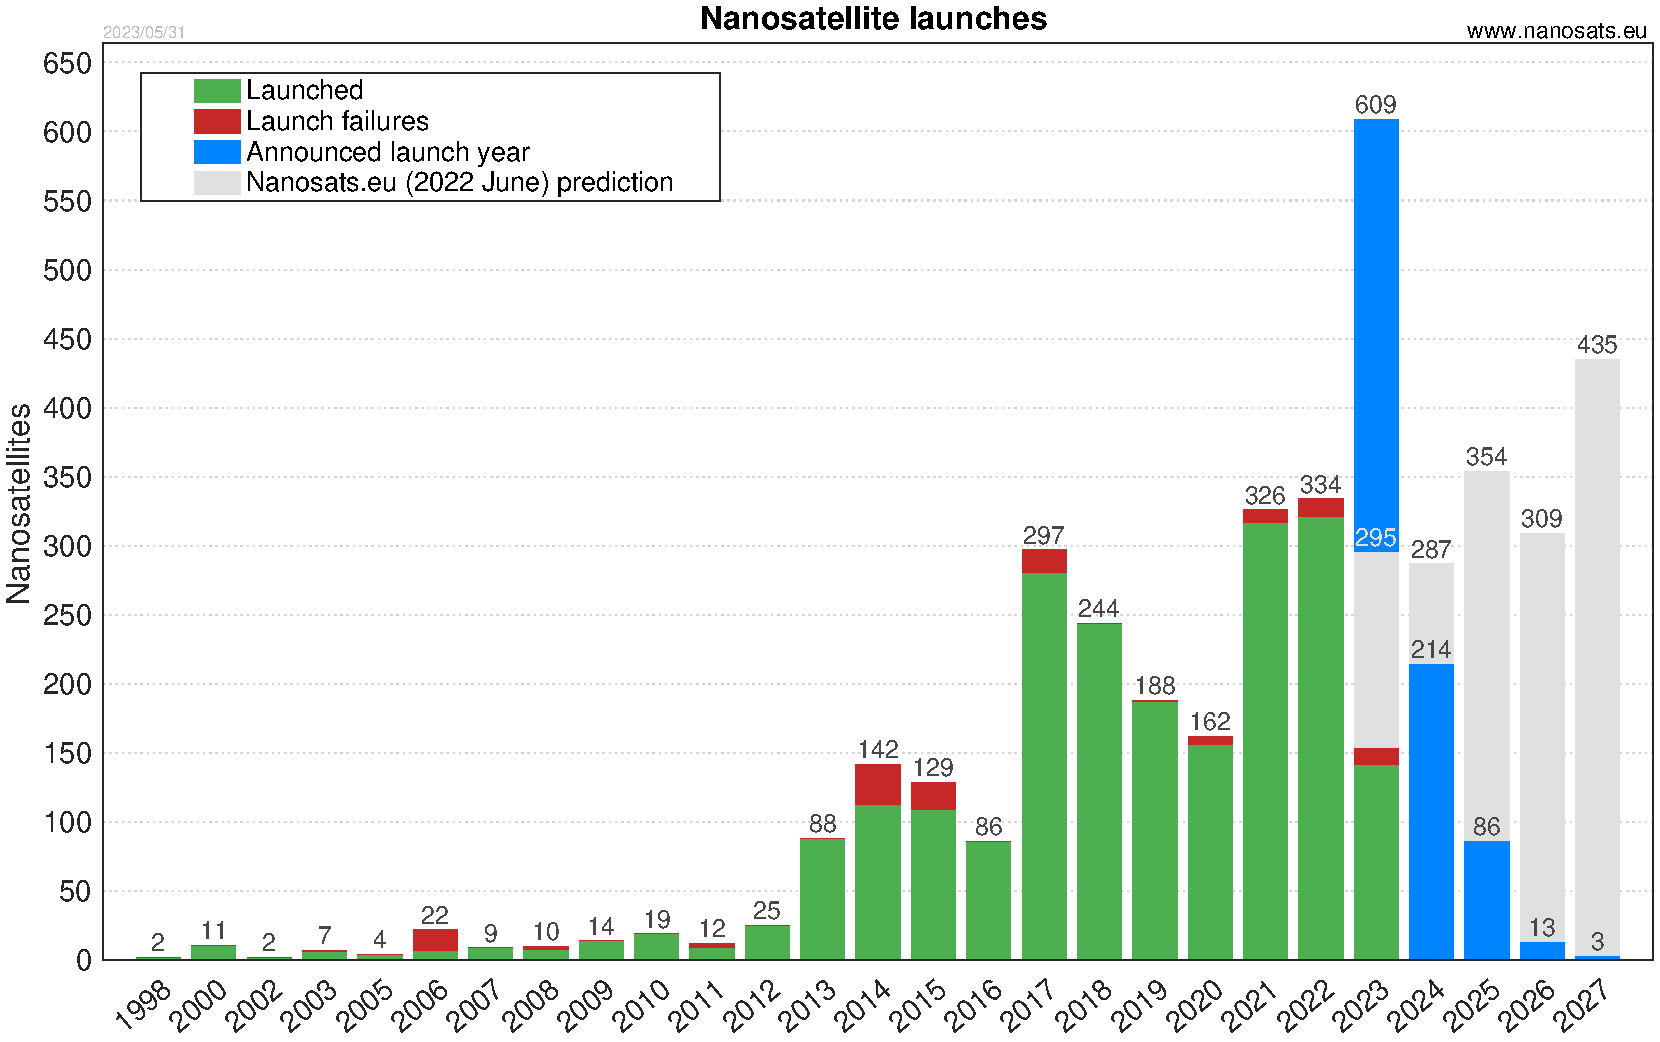
\includegraphics[width=\columnwidth]{figures/Nanosats_years_2023-05-31}
        \caption{Nanosatellite launches (2023/05/31) \cite{nanosatseu}.}
        \label{fig:cubesat-launches}
    \end{center}
\end{figure}

With a considerably lower cost, mainly due to the use of lower orbits such as LEO\nomenclature{\textbf{LEO}}{Low Earth Orbit.} (Low Earth Orbit) and COTS (Commercial Off-The-Shelf) components, it is becoming easier to develop and put this type of satellite into operation in space.

A standard that has dominated the nanosatellite market is the CubeSat standard \cite{cds}, which standardizes various physical characteristics for these types of satellites. This standard not only standardizes the space subsystems available on the market but also standardizes the launchers, which reduces the cost of launching a nanosatellite, which is one of the biggest costs within this type of project.

\section{Constellations}

Along with the rise of CubeSats, constellations of small satellites have emerged and grown in recent years. The low cost of this type of satellite, along with a significant recent increase in the number of launches, has also made it easier to create and deploy constellations of small satellites in low Earth orbit. With dozens or even hundreds of satellites in orbit, it is possible to achieve nearly constant coverage over the entire world. The chart in \autoref{fig:constellations} shows the status of the main nanosatellite constellations that are already in operation or planned for deployment.

\begin{figure}[!ht]
    \begin{center}
        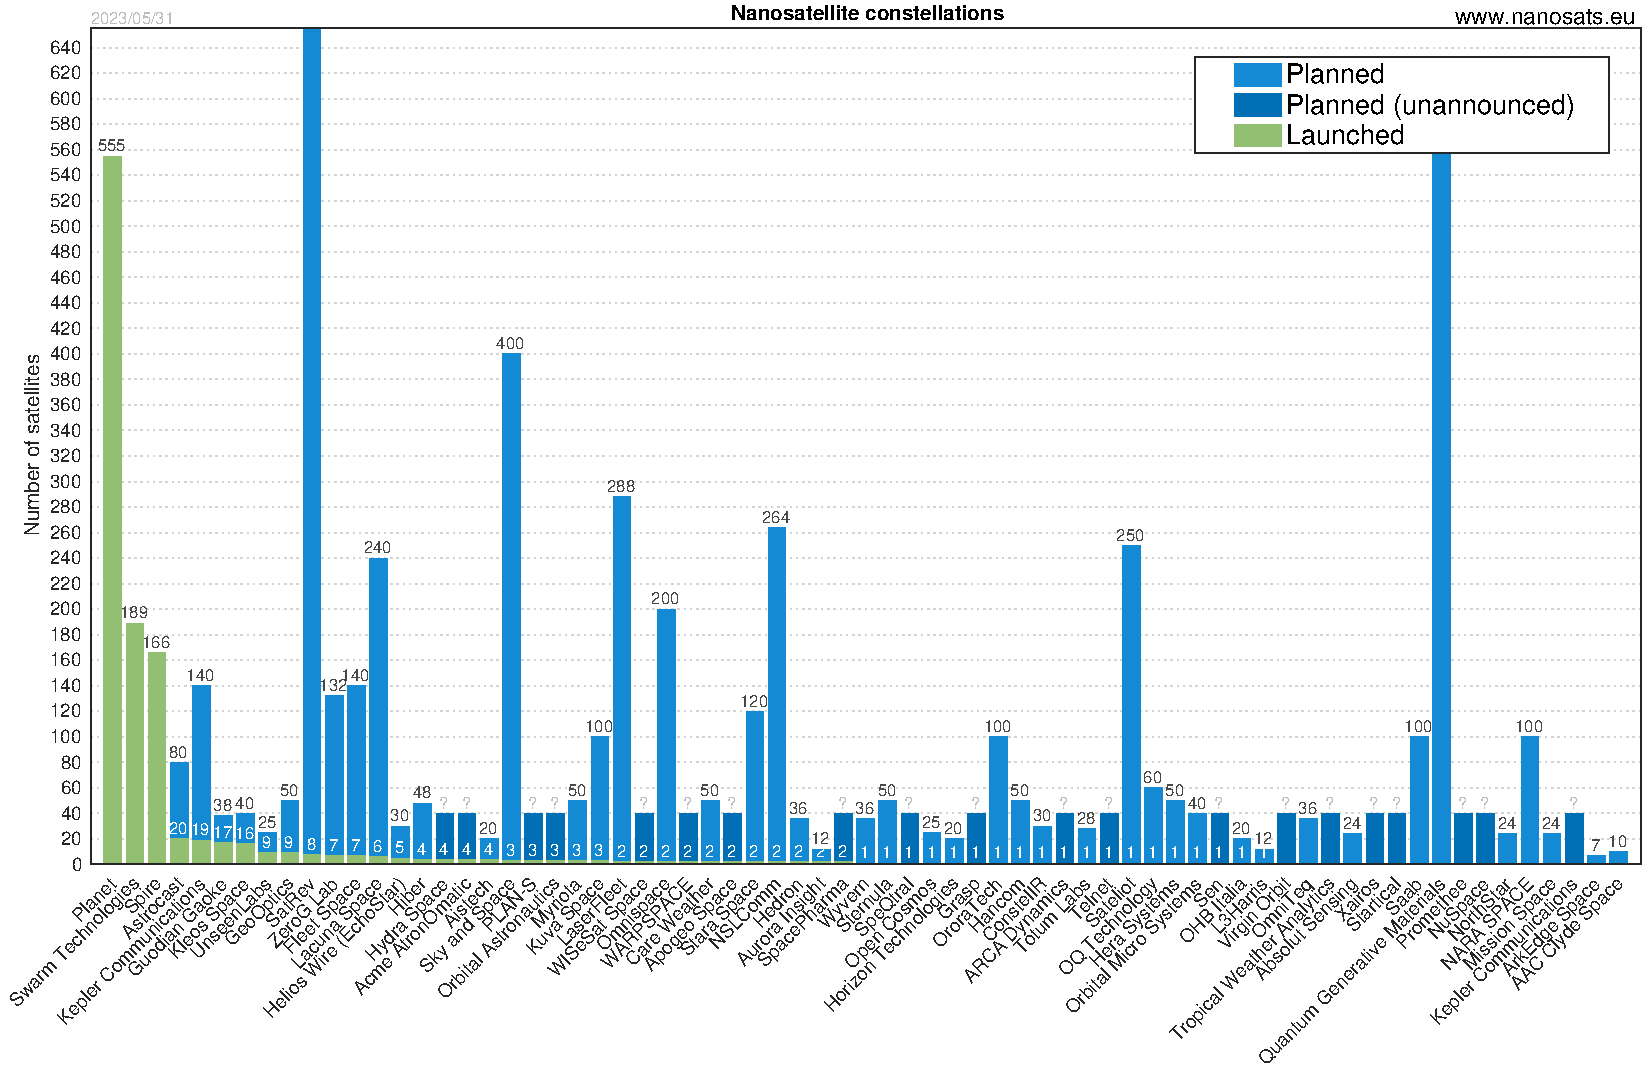
\includegraphics[width=\columnwidth]{figures/Nanosats_constellations_2023-05-31}
        \caption{Nanosatellite constellations (2023/05/31) \cite{nanosatseu}.}
        \label{fig:constellations}
    \end{center}
\end{figure}

\section{Motivation}

%Considerando o contexto apresentado acima a respeito do crescimento atual da utilização de pequenos satélites e da implatação de constelações dos mesmos, e ainda o rápido crescimento de dispositivos com necessidade de conexão a internet, denominadados Internet das Coisas (ou \textit{Internet of Things}, IoT), e outras tipos de tecnologias em ascenção como veículos autônomos, uma possível utilização dos nanossatélites seria em sistemas de navegação e localização, seja de cobertura específica para uma área, ou com cobertura global (GNSS).

%Considerando o contexto apresentado acima a respeito do crescimento atual da utilização de pequenos satélites e da implatação de constelações dos mesmos, uma possível utilização dos nanossatélites seria em sistemas de navegação e localização, seja de cobertura específica para uma área, ou com cobertura global (GNSS). O rápido crescimento de dispositivos com necessidade de conexão a internet, denominadados Internet das Coisas (ou \textit{Internet of Things}, IoT), e outras tipos de tecnologias em ascenção como veículos autônomos, tornam ainda mais atraente o uso desses tipos de satélites para aplicações desse tipo.

%Atualmente, os sistemas de navegação por satélite são compostos por satélites de grande porte operando em altitudes elevadas, normalmente em órbitas médias (MEO) ou até em órbitas geoestacionárias. Como será apresentado neste trabalho, a utilização de satélites de pequeno porte neste tipo de aplicação pode trazer algumas vantagens como um menor custo de implantação e operação, uma maior cobertura territorial e maior precisão, e até mesmos a simplificação de receptores em terra.

Considering the context presented above regarding the current growth of the use of small satellites and the implementation of constellations of these, a possible use of nanosatellites would be in navigation and location systems, either with specific coverage for an area or with global coverage (GNSS). The rapid growth of devices that require internet connection, known as the Internet of Things (IoT), and other emerging technologies such as autonomous vehicles, make the use of these types of satellites even more attractive for applications of this kind.

Currently, satellite navigation systems are composed of large satellites operating at high altitudes, typically in Medium Earth Orbits (MEO) or even in geostationary orbits (GEO). As will be presented in this work, the use of small satellites in this type of application can bring some advantages such as lower deployment and operation costs, greater territorial coverage and precision, and even the simplification of ground receivers.

\section{Objectives}

%Este trabalho tem como principal objetivo avaliar a possibilidade e viabilidade da implantação de um sistema de geolocalização baseado em satélites de pequeno porte, operando principalmente na forma de uma constelação em órbita baixa. O trabalho apresenta um estudo de órbita (como por exemplo o número de satélites necessários para um sistema desse tipo visando uma cobertura global), tecnologias disponíveis para a referência de tempo do sistema e outros subsistemas do satélite (neste caso especificamente para satélite de pequeno porte).

%Também tem-se como objetivo, o desenvolvimento de uma carga útil para a geração e transmissão de sinais de GNSS, a ser utilizada em um satélite de pequeno porte em uma missão projetada especificamente para testar e verificar o desempenho do sistema proposto.

The main objective of this work is to evaluate the possibility and feasibility of deploying a geolocation system based on small satellites, mainly operating in the form of a low Earth orbit constellation. The work presents an orbit study (such as the number of satellites required for such a system aiming at global coverage), technologies available for system time reference and other satellite subsystems (in this case, specifically for small satellites).

Another objective is to develop a payload for generating and transmitting GNSS signals, to be used on a small satellite in a mission designed specifically to test and verify the performance of the proposed system.

\section{Original contribution}

%Este trabalho tem como principal contribuição avaliar a viabilidade da implantação de um sistema de geolocalização baseado em pequenos satélites, explorando a possíveis tecnologias que podem ser utilizadas para a simplificação e/ou miniaturização dos componentes envolvidos do segmento espacial de um sistema deste tipo, um estudo de possíveis órbitas e tamanhos de constelação, e os requisitos necessários para os satélites do sistema.

%Como será demonstrado, há poucos trabalhos ou pesquisas acadêmicas semelhantes a este publicados até então. Já existem empresas explorando a possibilidade do uso de pequenos satélites em órbita baixa para o emprego de redes privadas de GNSS, mas nenhuma rede deste tipo já encontra-se em operação, todas encontram-se atualmente em fase de estudo e desenvolvimento. Portanto este trabalho pode ser considerado inovador e apresenta novos dados e informações para o área.

This work's main contribution is to evaluate the feasibility of implementing a geolocation system based on small satellites, exploring possible technologies that can be used to simplify and/or miniaturize the components involved in the space segment of such a system, a study of possible orbits and constellation sizes, and the necessary requirements for the system's satellites.

As will be demonstrated, there are few similar academic works or research published to date. There are already companies exploring the possibility of using small satellites in low orbit for the deployment of private GNSS networks, but no network of this type is currently in operation, all are still in the study and development phase. Therefore, this work can be considered innovative and presents new data and information for the field.

\section{Work organization}

%O \autoref{ch:related-work} apresenta uma revisão do estado da arte, comentando sobre o funcionamento de cada uma das redes atuais de GNSS, e apresentando os principais trabalhos relacionados, tanto a respeito da utilização de pequenos satéltes para este tipo de aplicação, quanto a repeito de tecnologias específicas que poderiam ser utilizadas para uma rede deste tipo.

%O \autoref{ch:problem-discussion} discute os principais problemas e questões a respeito da utilização de pequenos satélites e constelações dos mesmos para solucionar este tipo de problema. Neste capítulo apresenta-se possíveis tecnologias que poderiam ser utilizadas, questões de desempenho, entre outros.

%Já o \autoref{ch:proposed-work}, apresenta de forma detalhada o trabalha proposto, discutindo-se as principais questões a serem levadas em consideração neste tipo de problema, possíveis soluções que podem ser exploradas e análises preliminares.

Chapter \ref{ch:related-work} presents a review of the state of the art, commenting on the functioning of each of the current GNSS networks, and presenting the main related works, both regarding the use of small satellites for this type of application and regarding specific technologies that could be used for a network of this type.

Chapter \ref{ch:problem-discussion} discusses the main problems and issues regarding the use of small satellites and constellations of them to solve this type of problem. This chapter presents possible technologies that could be used, performance issues, among others.

Finally, \autoref{ch:proposed-work} presents in detail the proposed work, discussing the main issues to be taken into consideration in this type of problem, possible solutions that can be explored, and preliminary analyses.
    %
% related-work.tex
%
% Copyright (C) 2023 by Universidade Federal de Santa Catarina.
%
% Towards the Conception of GNSS Networks Based on Small Satellites
%
% This work is licensed under the Creative Commons Attribution-ShareAlike 4.0
% International License. To view a copy of this license,
% visit http://creativecommons.org/licenses/by-sa/4.0/.
%

%
% \brief Related works section.
%
% \author Gabriel Mariano Marcelino <gabriel.mm8@gmail.com>
%
% \version 1.1.0
%
% \date 2021/06/14
%

\chapter{Related Work} \label{ch:related-work}

%Este capítulo apresenta um resumo dos principais trabalhos relacionados e a situação atual das redes de GNSS no mundo, apresentando-se o histórico e status das redes atualmente em operação, e projetos atualmente em andamento e que possivelmente serão implementados ou entraram em operação no futuro, tanto com a utilização de satélites convencionais quanto com satélites de pequeno porte. Além de trabalhos relacionados estudando a viabilidade e possíveis soluções para a implantação destas redes através de uso de pequenos satélites e/ou mega-constelações.

This chapter presents a summary of the main related works and the current situation of GNSS networks in the world, presenting the history and status of the networks currently in operation, as well as ongoing projects that may be implemented or put into operation in the future, both using conventional satellites and small satellites. In addition, it includes related works studying the feasibility and possible solutions for the deployment of these networks through the use of small satellites and/or mega-constellations.

\section{Current GNSS networks}

%Atualmente existem quatro redes de GNSS em operação: GPS\nomenclature{\textbf{GPS}}{Global Positioning System}, GLONASS\nomenclature{\textbf{GLONASS}}{\textit{Globalnaya navigatsionnaya sputnikovaya sistema}}, Galileo e BDS\nomenclature{\textbf{BDS}}{BeiDou Navigation Satellite System}. Além de mais duas redes locais, que operam de forma limitada a uma região específica: QZSS\nomenclature{\textbf{QZSS}}{Quasi-Zenith Satellite System} e IRNSS\nomenclature{\textbf{IRNSS}}{Indian Regional Navigation Satellite System}. Abaixo, encontra-se uma descrição e mais informações sobre cada uma dessas redes.

Currently, there are four GNSS networks in operation: GPS\nomenclature{\textbf{GPS}}{Global Positioning System.}, GLONASS\nomenclature{\textbf{GLONASS}}{\textit{Globalnaya navigatsionnaya sputnikovaya sistema.}}, Galileo, and BDS\nomenclature{\textbf{BDS}}{BeiDou Navigation Satellite System.}. In addition to two local networks, which operate in a limited way to a specific region: QZSS\nomenclature{\textbf{QZSS}}{Quasi-Zenith Satellite System.} and IRNSS\nomenclature{\textbf{IRNSS}}{Indian Regional Navigation Satellite System.}. Below there is a description and further information about each of these networks.

\subsection{GPS}

%O GPS \cite{gps}, ou Global Positioning System, é o sistema de GNSS desenvolvido e mantido pelos Estados Unidos. Foi o primeiro sistema de navegação global por satélite a ser desenvolvido e entrar em operação, tendo o projeto sido iniciado no início da década de 1970, com os primeiros satélites lançados em 1978. A rede se tornou operacional em 1995 e teve custo total de 10 bilhões de dólares. Atualmente possuí 24 satélites em operação, operando a uma altitude de aproximadamente 20200 quilômetros (MEO\nomenclature{\textbf{MEO}}{Medium Earth Orbit}) e com a premissa de se ter sempre pelo menos quatro satélites cobrindo qualquer ponto do planeta \cite{el-rabbany2002}.

GPS \cite{gps}, or Global Positioning System, is the GNSS system developed and maintained by the United States. It was the first global satellite navigation system to be developed and put into operation, with the project starting in the early 1970s and the first satellites launched in 1978. The network became operational in 1995 and had a total cost of approximately 10 billion dollars. Currently, it has 24 satellites in operation, operating at an altitude of approximately 20,200 kilometers (MEO\nomenclature{\textbf{MEO}}{Medium Earth Orbit.}) and with the premise of always having at least four satellites covering any point on the planet. The 24 satellites are divided in six orbital planes, with four satellites per plane \cite{el-rabbany2002}.

%Atualmente o sistema é de uso civil e militar, mas até a década de 2000, o sistema possuía precisão propositalmente limitada para dispositivos de uso civil, sendo seu uso em capacidade máxima destinado somente a aplicações militares. Por questões de segurança, erros propositais eram induzidos aos sinais transmitidos de forma que receptores de uso geral não possuíssem precisão menor que 90 metros.

Currently, the system is used for both civilian and military purposes, but until the 2000s, the system deliberately had limited precision for civilian use devices, with its maximum capacity use intended only for military applications. For security reasons, intentional errors were induced into the transmitted signals so that general-use receivers did not have accuracy less than 90 meters.

%O GPS opera em três frequências diferentes: 1575,42, 1227,6 e 1176,45 MHz, com larguras de banda igual a 15,345, 11 e 12,5 MHz, respectivamente. Utilizando essas frequências, operam quatro tipos de sinais: L1 C/A, L1C, L2 C, L2 P e L5 (os sinais L2 C e L2 P operam na mesma frequência: 1227,6 MHz). Os sinais são transmitidos através da modulação BPSK.

GPS operates at three different frequencies: 1575.42, 1227.6, and 1176.45 MHz, with bandwidths of 15.345, 11, and 12.5 MHz, respectively. Four types of signals are used: L1 C/A, L1C, L2 C, L2 P, and L5 (L2 C and L2 P signals operate at the same frequency: 1227.6 MHz). The signals are transmitted through BPSK modulation.

To control the operation of the network, the ground segment of the system is divided into three groups: master control station (MCS\nomenclature{\textbf{MCS}}{Master Control Station.}), monitor stations and ground control stations. The MCS is composed of a single station lacated in Colorado Springs (Colorado, USA), and is the center of the GPS operations.

The monitor stations are composed by five stations with a precisely known locations, located in Colorado Spring (same place as the MCS), Hawaii, Kwajalein, Diego Garcia and Ascension Island. These monitor stations have a high-quality GPS receivers and high-precision cesium clocks, mainly for tracking all satellites of the network in real-time. Some of them are also equiped with uplinks for uploading telecommands and informations for the satellites, and all of them are operated remotely by the MCS.

The locations and stations of the ground segment of the GPS network is illustrated in \autoref{fig:gps-ground-segment}.

\begin{figure}[!ht]
    \begin{center}
        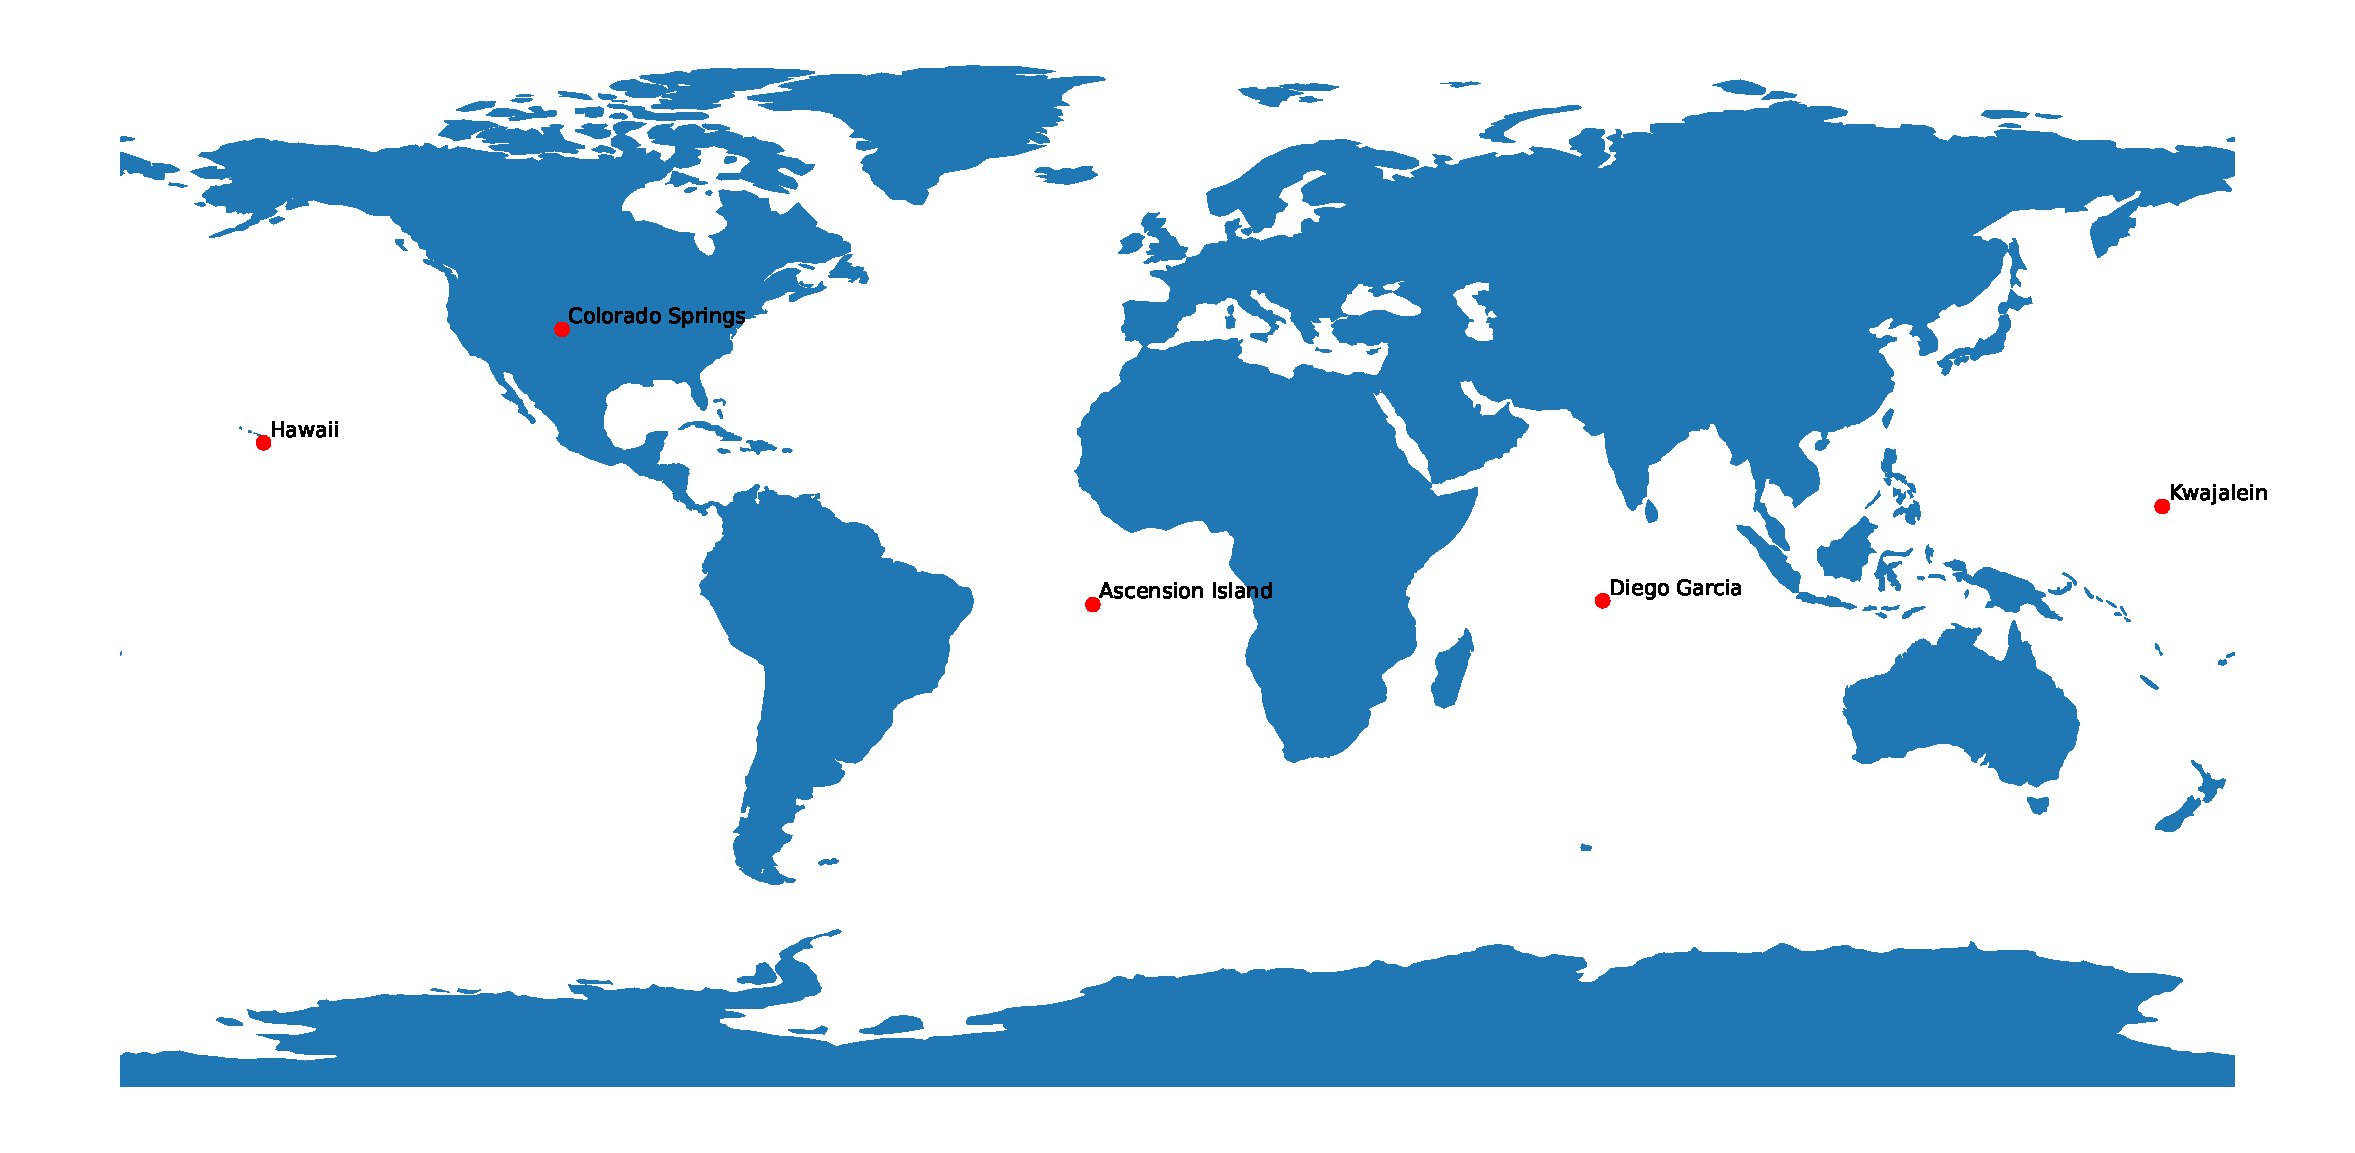
\includegraphics[width=\columnwidth]{curves/gps-ground-segment}
        \caption{Ground segment of the GPS network (adapted from \cite{el-rabbany2002}).}
        \label{fig:gps-ground-segment}
    \end{center}
\end{figure}

\subsection{GLONASS}

%O GLONASS, sigla de \textit{Globalnaya navigatsionnaya sputnikovaya sistema} (ou Sistema de Navegação Global por Satélite) \cite{glonass}, é o sistema de GNSS criado e mantido pela Rússia. Este foi o segundo sistema de navegação global a entrar em operação, logo após o GPS, ainda durante o período da União Soviética.

%O projeto começou a ser desenvolvido em 1976, ainda na União Soviética. A implantação do sistema iniciou em 1982, e foi até 1995. Este é o projeto é o mais caro mantido pela agência espacial russa (Roscosmos), consumindo atualmente um terço do seu orçamento.

%O GLONASS opera em uma órbita circula a uma altitude de 19100 km e com uma inclinação de 64,8$^{\circ}$, resultando em período de 11 horas e 15 minutos. Sendo um sistema desenvolvido principalmente para cobrir o território russo (mas além disso, com cobertura global), este é adequado para operações em altas latitudes, onde o GPS pode apresentar problemas \cite{polischuk2002}.

%O GLONASS opera com quatro tipos de sinais: L1 C/A (1598,0625-1609,3125 MHz), L2 C (1242,9375-1251,6875 MHz), L2 P (1242,9375-1251,6875 MHz) e L3 OC (1202,025 MHz). Da mesma forma que o GPS, os sinais são transmitidos através da modulação BPSK.

%Atualmente, é comum o uso de receptores que são compatíveis tanto com GPS quanto com o GLONASS. Desta forma, tem-se uma maior disponibilidade de satélites, fazendo com que tenha-se uma maior rapidez na obtenção dos dados de posicionamento e uma maior precisão destes dados. Receptores deste tipo são mais robustos que receptores operando em uma única rede \cite{angrisano2012}.

GLONASS, which stands for \textit{Globalnaya navigatsionnaya sputnikovaya sistema} (or Global Navigation Satellite System in english) \cite{glonass}, is the GNSS system created and maintained by Russia. This was the second global navigation system to enter operation, right after GPS, still during the Soviet Union period.

The project started to be developed in 1976, still in the Soviet Union, based on the experiences with the Doppler satellite system Tsikada \cite{hofmann-wellenhof2007}. The system deployment started in 1982 and went until 1995. This is the most expensive project maintained by the Russian space agency (Roscosmos), currently consuming one-third of its budget.

GLONASS is originally a military-use system, for this reason, few information about the system was made available to the public during its early days. In 1988, a paper with technical information about the system was presented. In 1995, the Russian government issued a decree making the system available for use worldwide, thus no longer being an exclusive system for the Russian armed forces \cite{hofmann-wellenhof2007}.

GLONASS operates in a circular orbit at an altitude of 19,100 km and with an inclination of 64.8$^\circ$, resulting in a period of 11 hours and 15 minutes. The constellation consists of 24 satellites in three orbital planes, with 21 satellites considered as active, and three as spare satellites. Each orbital plane has eight equally spaced satellites \cite{hofmann-wellenhof2007}. Being a system developed mainly to cover the Russian territory (but also with global coverage), it is suitable for operations at high latitudes, where GPS can present problems \cite{polischuk2002}.

GLONASS operates with four types of signals: L1 C/A (1598.0625-1609.3125 MHz), L2 C (1242.9375-1251.6875 MHz), L2 P (1242.9375-1251.6875 MHz), and L3 OC (1202.025 MHz). Similarly to GPS, the signals are transmitted through BPSK modulation.

The satellites of this system follows an specification list described as below \cite{hofmann-wellenhof2007}:

\begin{itemize}
    \item Lifetime of at least three years
    \item Satellites mass of 1,415 kg
    \item Mass of the payload of 180 kg
    \item Power supply of 1,000 W
    \item Power consumption of the payload of 600 W
    \item Clock precision of 5 $\times$ 10$^{-13}$
    \item Attitude control system with an accuracy of 0.5$^{\circ}$
    \item Pointing accuracy of the solar panel of 5$^{\circ}$
\end{itemize}

The ground segment of the system is mostly installed over Russian territory, but some stations are located in countries that were part of the Soviet Union. The system control center, where the entire system is coordinated, is located in a military complex at the Krasnoznamensk Space Center near Moscow. The system time is controlled by the central synchronizer, also located in the Moscow region. The telemetry and telecommand stations, where communication with the satellites of the constellation occurs, are composed of four stations installed over Russian territory: St. Petersburg, Schelkovo, Yenisseysk (Siberia), and Komsomolsk-na-Amure (Far East). There are also five supplementary laser stations located mostly outside of Russian territory: one in Komsomolsk-na-Amure (inside Russia) and four others in Kazakhstan, Ukraine (two stations), and Uzbekistan \cite{hofmann-wellenhof2007}.

Currently, the use of receivers that are compatible with both GPS and GLONASS is common. In this way, there is a greater availability of satellites, resulting in faster data acquisition and greater precision of this data. Receivers of this type are more robust than those operating on a single network \cite{angrisano2012}.

\subsection{Galileo}

%O Galileo é o sistema de GNSS criado pela união europeia e mantido pela Agência Espacial Europeia (ESA), que começou a sua operação em 2016. O projeto começou a ser desenvolvido em 1999 e teve como principal objetivo desenvolver um sistema de posicionamento global de alta precisão independente dos sistemas GPS e GLONASS, levando em conta principalmente razões políticas e militares.

Galileo is the GNSS system created by the European Union and maintained by the European Space Agency (ESA), which started its operation in 2016. The project began to be developed in 1999 and had as its main objective to develop a high-precision global positioning system independent of the GPS and GLONASS systems, taking into account mainly political and military reasons.

%O sistema operara oferencendo dois tipos de serviço: um de precisão mais baixa aberto e gratuito, e outro de precisão mais alta de uso limitado e restrito. A constelação completa do sistema Galileo é composta por 24 satélites.

The system offers two types of service: one with lower precision, open and free, and another with higher precision, limited and restricted use. The complete constellation of the Galileo system consists of 30 satellites, considering 3 as spare. They are divided into three orbital planes (nearly circular orbits, MEO) with an inclination of 56$^{\circ}$. Considering the nominal opearion, a minimum of six satellites are guaranteed to be viewed at any place of the world \cite{hofmann-wellenhof2007}.

%O sistema funciona através de três tipos de sinais: E1 (1575,42 MHz), E5 (1191,795 MHz) e E6 (1278,75 MHz). O sinal E5 é subdividido em dois outros: E5a (1176,45 MHz) e E5b (1207,14 MHz).

The system operates through three types of signals: E1 (1575.42 MHz), E5 (1191.795 MHz), and E6 (1278.75 MHz). The E5 signal is subdivided into two others: E5a (1176.45 MHz) and E5b (1207.14 MHz). The configuration of the signals are presented in \autoref{tab:galileo-signals}.

\begin{table*}[!ht]
    \centering
    \begin{tabular}{lcc}
        \toprule[1.5pt]
        \textbf{Signal} & \textbf{Frequency} & \textbf{Modulation} \\
        \midrule
        E1  & 1575,42 MHz & CBOC \\
        E5a & 1176,45 MHz & AltBOC \\
        E5b & 1207,14 MHz & AltBOC \\
        E6  & 1278,75 MHz & BPSK \\
        \bottomrule[1.5pt]
    \end{tabular}
    \caption{Galileo signals configuration.}
    \label{tab:galileo-signals}
\end{table*}

%Atualmente, boa parte dos receptores GNSS comerciais e de uso civil têm suporte a rede Galileo. Por exemplo, grande parte dos smartphones modernos têm capacidade de trabalhar com múltiplas redes de GNSS, sendo a Galileo uma delas.

The satellites of the Galileo system carry two types of payloads: the main navigation payload and the SAR\nomenclature{\textbf{SAR}}{Search And Rescue.} payload. The first one is responsible for transmitting the Galileo signals, including all the needed equipment for that and the L-band antenna. The second payload receives emergency signals from equipments on Earth, redirecting them to ground stations through the L-Band link. The Galileo satellites have a size of approximately 2.7 $\times$ 1.2 $\times$ 1.1 m, and a weight of 730 kg. Besides a predicted lifetime of 12 years. A block diagram of the satellites of the Galileo constellation is available in \autoref{fig:galileo-satellite-bd}.

\begin{figure}[!ht]
    \begin{center}
        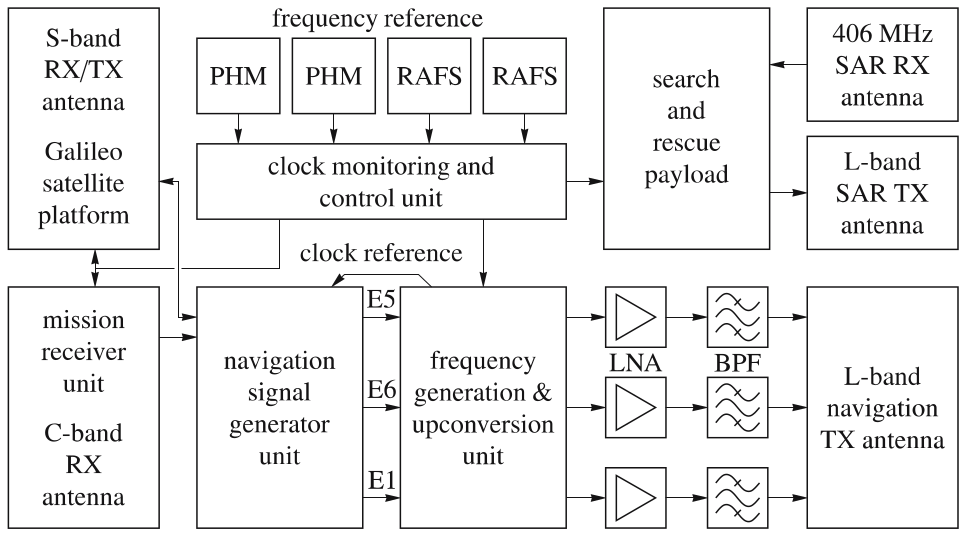
\includegraphics[width=\columnwidth]{figures/galileo-satellite-bd}
        \caption{Block diagram of a Galileo satellite \cite{hofmann-wellenhof2007}.}
        \label{fig:galileo-satellite-bd}
    \end{center}
\end{figure}

The ground segment is composed by:

\begin{itemize}
    \item Two control centers (Ground Control Center, or GCC)
    \item Five telemetry, tracking and control stations (TT\&C)
    \item Nine uplink stations operating in C-Band (ULS)
    \item Aproximately 40 sensor stations (GSS)
\end{itemize}

A map with the stations of the ground segment of the Galileo system is presented in \autoref{fig:galileo-ground-segment}.

\begin{figure}[!ht]
    \begin{center}
        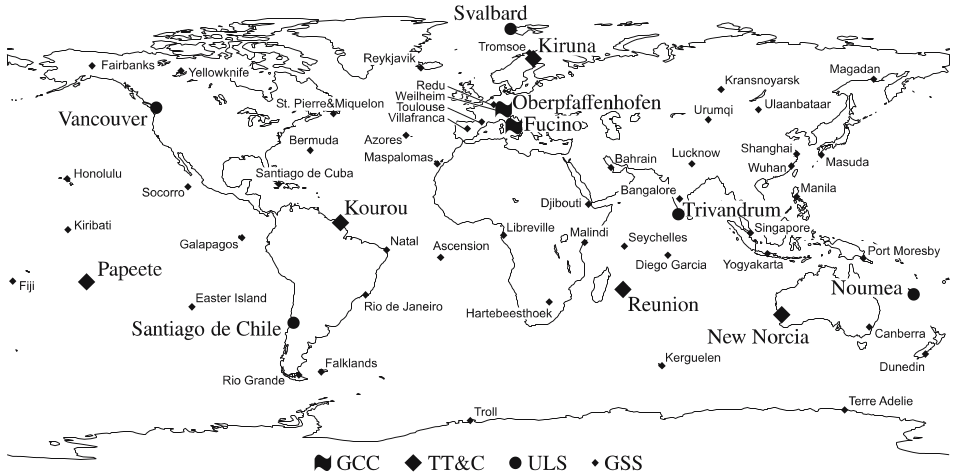
\includegraphics[width=\columnwidth]{figures/galileo-ground-segment}
        \caption{Ground segment of the Galileo system \cite{hofmann-wellenhof2007}.}
        \label{fig:galileo-ground-segment}
    \end{center}
\end{figure}

As can be seen, the ground infrastructure of the Galileo system highly robust in comparison with the other gelolocalization systems.

Currently, a large portion of commercial and civil GNSS receivers support the Galileo network. For example, most modern smartphones have the capability to work with multiple GNSS networks, including Galileo.

\subsection{BDS}

%O \textit{BeiDou Navigation Satellite System}, ou BDS \cite{beidou}, é o sistema de GNSS chinês.

%BeiDou, or BDS, is a global GNSS owned and operated by the People's Republic of China. BDS was formally commissioned in 2020. The operational system consists of 35 satellites. BDS was previously called Compass.

The Beidou Navigation Satellite System (BDS) \cite{beidou} a global navigation satellite system (GNSS) developed by China. Beidou, which means “Big Dipper” in Chinese, is also known as the Chinese Compass. The system consists of two separate satellite constellations: the regional Beidou-1 system and the global Beidou-2 system, which became fully operational in 2020.

The Beidou-1 system, which consists of four satellites, started operating in 2000. The Asia-Pacific area and China are its primary markets for positioning, navigation, and timing services. The GPS and GLONASS systems are compatible with the two frequencies used by the system, L1 and L2. A location accuracy of roughly 10 meters horizontally and 15 meters vertically, as well as a timing accuracy of roughly 10 nanoseconds, are provided by the Beidou-1 system.

There are 35 satellites total in the global Beidou-2 constellation, both geostationary and non-geostationary. The system offers positioning, navigation, and timing services with global coverage. Three frequencies—L1, L2, and L5—are used by the system for operation, and they are all compatible with other GNSS systems. The Beidou-2 system offers timing accuracy of around 20 to 30 nanoseconds, and positioning accuracy of roughly 2.5 meters horizontally and 5 meters vertically.

The Beidou system is made to be used for a variety of purposes, including commercial, civil, and military ones. In fields including transportation, surveying and mapping, precision agriculture, and disaster assistance, it is anticipated to have significant uses.

The Beidou Satellite-Based Augmentation System is a satellite-based augmentation system (SBAS\nomenclature{\textbf{SBAS}}{Satellite-Based Augmentation System.}) that the Beidou system offers in addition to GNSS capabilities (BDSBAS). The Beidou system's positioning, navigation, and timing services will be more accurate and dependable thanks to the BDSBAS.

Overall, China's development of cutting-edge space technologies has advanced thanks to the Beidou GNSS system. The technology is positioned to have a significant impact on navigation and location in the future thanks to its wide variety of applications and global coverage.

\section{Local networks}

Another type of network also in operation today is the network that operates locally, covering a specific region of the globe, called Regional Navigation Satellite System (RNSS\nomenclature{\textbf{RNSS}}{Regional Navigation Satellite System.}). With this characteristic, there are two in operation nowadays: QZSS and IRNSS networks. Both are described below.

\subsection{QZSS}

%The Quasi-Zenith Satellite System \cite{qzss} (QZSS, or also know as Michibiki) is a local positioning system developed by the Japanese government covering part of Asia and Oceania, focusing primordially on the japanese territory. The objective of this system is to improve the GPS system coverage in the region with higher stability and precision. Currently, the system is composed by four satellites (QZS-1, 2, 3 and 4) and it is compatible with the GPS, but an independent system is also planned to be operational with seven satellites in 2023.

%The QZSS operates with one geostationaty satellite and three in a Tundra highly inclined, slightly elliptical, geosynchronous orbit, with each satellite 120$^{\circ}$ apart from each other. quasi-zenith orbit (QZO\nomenclature{\textbf{QZO}}{Quasi-Zenith Orbit}) scheme. This orbit is illustrade in \autoref{fig:qzss-orbit}.

The Quasi-Zenith Satellite System (QZSS) \cite{qzss} is a satellite-based positioning system developed by the Japanese government. It consists of a constellation of four satellites, one in geostationary orbit and three in a highly inclined elliptical orbit that covers Japan and the surrounding regions.

The QZSS system is designed to provide enhanced positioning accuracy and reliability, particularly in urban areas and mountainous terrain where satellite signals may be obstructed or weakened. The QZSS system is also designed to work in conjunction with other satellite positioning systems, such as GPS and GLONASS, to improve overall accuracy and reduce signal interference.

One of the unique features of the QZSS system is its use of a ``quasi-zenith'' orbit for its three inclined satellites. This means that the satellites spend a significant amount of time near the zenith, or highest point in the sky, which allows them to broadcast signals that are less obstructed by buildings and other obstructions. This orbit is illustrade in \autoref{fig:qzss-orbit}.

\begin{figure}[!ht]
    \begin{center}
        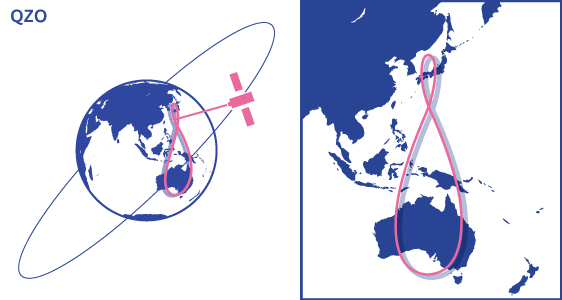
\includegraphics[width=0.8\columnwidth]{figures/qzss-orbit}
        \caption{Quasi-Zenith orbit of the QZSS network \cite{qzss}.}
        \label{fig:qzss-orbit}
    \end{center}
\end{figure}

The orbital elements of the QZSS satellites are available in \autoref{tab:qzss-orbit-config}.

\begin{table*}[!ht]
    \centering
    \begin{tabular}{lc}
        \toprule[1.5pt]
        \textbf{Keplerian Elements} & \textbf{Value} \\
        \midrule
        Epoch                                   & 26 December 2009, 12:00 UTC \\
        Semimajor                               & 42164 km \\
        Eccentricity                            & $0,075 \pm 0,015$ \\
        Inclination                             & $43 \pm 4^{\circ}$ \\
        Right ascension of the ascending node   & $195^{\circ}$ \\
        Argument of perigee                     & $270 \pm 2^{\circ}$ \\
        Mean anomaly                            & $305^{\circ}$ \\
        Central longitude of ground trace       & $135\ E \pm 5^{\circ}$ \\
        \bottomrule[1.5pt]
    \end{tabular}
    \caption{Orbit configuration of the QZSS.}
    \label{tab:qzss-orbit-config}
\end{table*}

The QZSS system is used for a variety of applications, including transportation, disaster response, agriculture, and surveying. The system has also been integrated into some consumer devices, such as smartphones and car navigation systems.

The QZSS system is considered an important strategic asset for Japan, and the government has plans to expand the constellation to seven satellites by 2023. This expansion will further enhance the system's accuracy and reliability and make it an even more valuable resource for users in Japan and beyond.

\subsection{IRNSS}

%The IRNSS (Indian Regional Navigation Satellite System) \cite{irnss} is a regional and independent nagivation system developed and maintained by India, focusing on covering mainly its territory. This network is currently composed by a constellation of seven satellites, three in a geostationaty orbit, and four in a geosynchronous orbit.

%IRNSS is a regional GNSS owned and operated by the Government of India. IRNSS is an autonomous system designed to cover the Indian region and 1500 km around the Indian mainland. The system consists of 7 satellites. In 2016, India renamed IRNSS as the Navigation Indian Constellation (NavIC, meaning ``sailor'' or ``navigator'').

The Indian Regional Navigation Satellite System (IRNSS) \cite{irnss}, also known as NavIC (Navigation with Indian Constellation), is a satellite-based positioning system developed by the Indian Space Research Organisation (ISRO). NavIC is designed to provide accurate and reliable positioning services to users in India and the surrounding regions.

The system consists of a constellation of seven satellites in orbit, three in geostationary orbit and four in geosynchronous orbit, covering the entire Indian subcontinent and extending up to 1,500 kilometers beyond its borders. NavIC is capable of providing a position accuracy of up to 5 meters, and the system is compatible with both GPS and GLONASS, allowing for greater redundancy and improved accuracy. A diagram of the IRNSS with the coverage area and the satellites can be seen in \autoref{fig:irnss}.

\begin{figure}[!ht]
    \begin{center}
        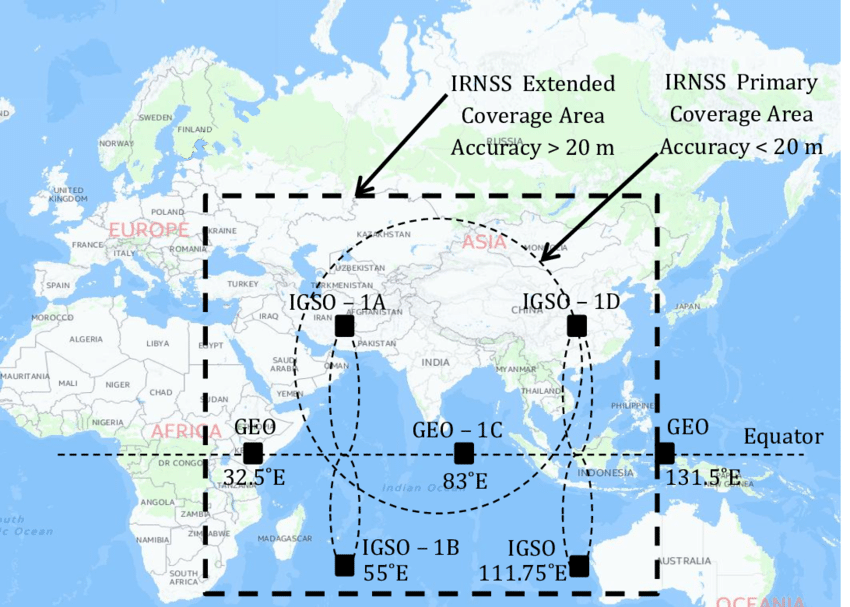
\includegraphics[width=0.8\columnwidth]{figures/irnss}
        \caption{IRNSS satellites and coverage of the system (adapted from \cite{thombre2015}).}
        \label{fig:irnss}
    \end{center}
\end{figure}

NavIC offers a wide range of applications, including vehicle tracking, maritime navigation, disaster management, and location-based services. The system is particularly useful in rural and remote areas of India, where traditional navigation systems may be unreliable or unavailable.

The Indian government has made NavIC available for civilian use, and several companies are already integrating the technology into their products and services. With the growing demand for accurate and reliable positioning information, NavIC is poised to become a major player in the global navigation satellite system market.

\subsection{KPS}

The Korea Positioning System (KPS\nomenclature{\textbf{KPS}}{Korea Positioning System.}) \cite{choi2020} is a satellite-based navigation system developed by the South Korean government. The KPS system is designed to provide positioning, navigation, and timing (PNT) services to users in South Korea and the surrounding regions.

%\begin{itemize}
%    \item GPS is a key component of the Korean national infrastructure, such as roads, power grid, timing, and national security
%    \item In the case of a looming crisis such as a conflict, signals can be blocked by countries with own GNSS system to prevent their enemy forces from using them
%    \item However, Korea does not have any navigation satellites, so totally depends on GNSS systems of other countries like GPS
%    \item This possibility necessitated the development of KPS
%\end{itemize}

%The Global Positioning System (GPS) is an essential technology for many countries, including South Korea. It plays a crucial role in the Korean national infrastructure, such as roads, power grids, timing, and national security.

One of the motivations for the development of this system, in that in times of crisis, such as a military conflict, countries with their own GNSS system could block the signals to prevent their enemy forces from using them. This situation raises concerns for South Korea, which relies entirely on GPS and other foreign GNSS systems. To address this issue, South Korea is developing its own GNSS system. The KPS aims to provide more accurate and reliable positioning information for Korean users, especially during emergencies when GPS signals could be blocked.

The KPS is also expected to promote technological independence and enhance the competitiveness of the Korean space industry. Moreover, it will contribute to the development of various industries that rely on positioning information, such as transportation, logistics, and agriculture.

In summary, the development of KPS is a significant step towards securing the nation's technological independence and strengthening its national security. With the launch of the KPS system, South Korea will join the group of countries with their own GNSS system. This system is still under development and is expected to be operational in the coming years.

\section{Comparison between systems}

Considering the information presented above about the navigation systems currently in operation (or already in implantation), \autoref{tab:networks-comparison} compares the main characteristics of all the systems presented.

\begin{landscape}

\begin{table*}[!ht]
    \centering
    \begin{tabular}{lccccccc}
        \toprule[1.5pt]
        \multirow{2}{*}{\textbf{Characteristic}} & \multicolumn{7}{c}{\textbf{Network}} \\
                                                 & \textbf{GPS} & \textbf{GLONASS} & \textbf{Galileo} & \textbf{BDS} & \textbf{QZSS} & \textbf{IRNSS} & \textbf{KPS} \\
        \midrule
        Coverage      & Global        & Global      & Global         & Global      & Regional    & Regional    & Regional \\
        Country       & United States & Russia      & European Union & China       & Japan       & India       & South Korea\\
        Satellites    & 32            & 24          & 30             & 30          & 4           & 7           & 3 \\
        Orbit         & MEO           & MEO         & MEO            & MEO         & GEO         & GEO/MEO     & LEO \\
        Altitude [km] & 20200         & 19100       & 23200          & 21000       & 39000       & 36000       & 1000 \\
        Bands         & L1, L2, L5    & L1, L2      & E1, E5a, E5b   & B1, B2, B3  & L1, L2C, L5 & L5, S       & K \\
        Launch year   & 1978          & 1982        & 2016           & 2000        & 2010        & 2013        & 2021 \\
        Accuracy [m]  & 5-10          & 5-10        & 1-5            & 5-10        & 1-5         & 5-10        & 5-10 \\
        Status        & Operational   & Operational & Operational    & Operational & Operational & Operational & Planned \\
        \bottomrule[1.5pt]
    \end{tabular}
    \caption{Comparison between the main global and regional navigation networks (situation in 2023).}
    \label{tab:networks-comparison}
\end{table*}

\end{landscape}

%        \multirow{6}{*}{Frequency [MHz]} & 1575,42 (L1 C/A)  & 1598,0625-1609,3125 (L1 C/A) & 1575,42 (E1)         & 1561,098 (B1l) & 1575,42 (L1 C/A/S) & 1176,45 (L5) \\
%                                         & 1227,6 (L2 C/P)   & 1242,9375-1251,6875 (L2 C/P) & 1176,45 (E5a)        & 1207,14 (B2l)  & 1227,6 (L2C)       &  \\
%                                         & 1176,45 (L5)      & 1202,025            (L3 OC)  & 1207,14 (E5b)        & 1268,52 (B3l)  & 1176,45 (L5)       &  \\
%                                         &                   &                              & 1191,795 (E5 AltBOC) & 1575,42 (B1C)  & 1278,75 (L6)       &  \\
%                                         &                   &                              & 1275,75 (E6)         & 1176,45 (B2a)  &                    &  \\
%                                         &                   &                              &                      & 1207,14 (B2b)  &                    &  \\

\section{Experimental GNSS networks}

%Recentemente, com o avanço dos nanossatélites, o crescimento de dispositivos com conectividade e a Internet das coisas (IoT), começou a surgir ideias de implantação de redes privadas e em baixa órbita de sistemas de GNSS, seja para atender propósitos específicos ou de uso geral. Considerando, começam a surgir iniciativas de empresas para a utilização de pequenos satélites para esse tipo de aplicação, o que vai de encontro a ideia principal deste trabalho.

Recently, with the advancement of nanosatellites, the growth of devices with connectivity and the Internet of Things (IoT), ideas for deploying private and low-orbit GNSS systems networks have emerged, either to serve specific or general purposes. Considering this, companies are starting to take initiatives to use small satellites for this type of application, which aligns with the main idea of this work.

%Dentre essas iniciativas, pode-se destacar duas startups que possuem propostas similares: TrustPoint\footnote{\href{https://www.trustpointgps.com/}{https://www.trustpointgps.com/}} e Xona Space Systems\footnote{\href{https://www.xonaspace.com/}{https://www.xonaspace.com/}}.

Among these initiatives, two startups with similar proposals can be highlighted: TrustPoint\footnote{\href{https://www.trustpointgps.com/}{https://www.trustpointgps.com/}} and Xona Space Systems\footnote{\href{https://www.xonaspace.com/}{https://www.xonaspace.com/}}.

%A primeira tem como proposta a criação de uma rede GNSS totalmente de uso comercial e com melhorias em relação ao GPS atual, como aumento de desempenho, melhorias de segurança e maior robustez. Mais especificamente, a proposta inclui um sistema anti-spoof and anti-jam, e um tempo menor para fixar o sinal. Além disso, para a implementação da rede propõe-se o uso de satélites de pequeno porte, do tipo microssatélite.

The first initiative proposes the creation of a completely commercial GNSS network with improvements over the current GPS, such as increased performance, improved security, and greater robustness. More specifically, the proposal includes an anti-spoof and anti-jam system, and a shorter time to fix the signal. In addition, the implementation of the network proposes the use of small satellites, such as microsatellites.

%Já a segunda \cite{aarestad2020}, propõe a implantação de redes privadas de GNSS, utilizando satélites em baixa órbita. Uma imagem conceitual de um dos satélites da rede pode ser vista na \autoref{fig:xona-satellite}.

The second one proposes the deployment of private GNSS networks, using satellites in low Earth orbit \cite{reid2020} \cite{reid2023}. A conceptual image of one of the network satellites can be seen in Figure \ref{fig:xona-satellite}.

\begin{figure}[!ht]
    \begin{center}
        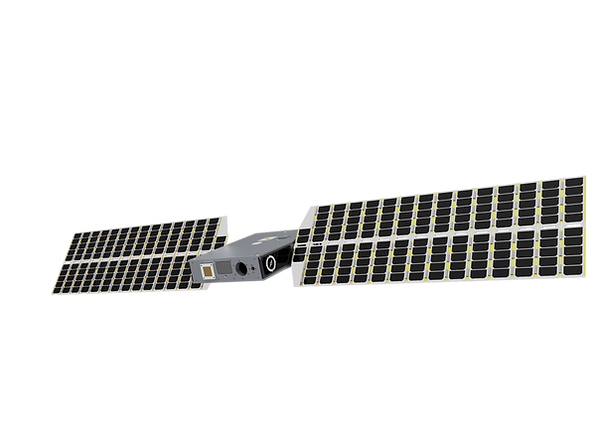
\includegraphics[width=0.8\columnwidth]{figures/xona-satellite}
        \caption{Xona Space Systems conceptual satellite.}
        \label{fig:xona-satellite}
    \end{center}
\end{figure}

%Considerando-se que ainda são projetos em estágio inicial e sendo desenvolvidos por empresas, não encontra-se disponível de forma pública informações mais técnicas e detalhadas sobre essas duas redes.

%Outros trabalhos ainda em fase pesquisa, também discutem a fusão de serviços de GNSS com outros tipos de serviço de telecomunicação, como por exemplo a adição de uma rede GNSS em megaconstelações como por exemplo a Starlink \cite{iannucci2022}.

Considering that they are still early-stage projects being developed by companies, more technical and detailed information about these two networks is not publicly available.

\section{Related works}

%Além das redes já consolidadas operando em órbitas mais altas e baseadas em satélites de grandes porte, há alguns trabalhos focados em tópicos específicos sobre a implantação de redes de geolocalização.

In addition to the already established networks operating in higher orbits and based on large satellites, there are some studies focused on specific topics regarding the deployment of geolocation networks.

Other research works still in progress also discuss the fusion of GNSS services with other types of telecommunication services, such as the addition of a GNSS network in mega-constellations like Starlink \cite{iannucci2022}.

%Já o trabalho de \cite{reid2018} apresenta um estudo sobre como constelações de satélites operando em órbita baixa (LEO) podem ser utilizadas para sistemas de navegação. O trabalho destaca as vantagens desse tipo de sistema, como por exemplo a operação com sinais com maior potência, o que permite uma melhor recepção em ambientes fechados, e uma maior robustez contra jamming. O trabalho também cita a principal desvantagem de sistemas operando nessas órbitas: a necessidade de um número maior de satélites para se obter uma cobertura global. Outro aspecto discutido é a menor incidência de radiação ionizante em órbitas baixas, o que torna possível por exemplo a utilização de componentes COTS\nomenclature{\textbf{COTS}}{Commercial-Off-The-Shelf.} (Commercial-Off-The-Shelf).

%Também existem trabalhos que exploram a utilização das redes de GNSS atuais em outros corpos estelares, como por exemplo a Lua \cite{capuano2015} \cite{delepaut2020}.

The work of \cite{reid2018} presents a study on how constellations of satellites operating in low Earth orbit (LEO) can be used for navigation systems. The paper highlights the advantages of this type of system, such as operating with higher power signals, which allows for better reception in indoor environments, and greater robustness against jamming. The work also mentions the main disadvantage of systems operating in these orbits: the need for a larger number of satellites to achieve global coverage. Another aspect discussed is the lower incidence of ionizing radiation in low orbits, which makes it possible, for example, to use Commercial-Off-The-Shelf (COTS\nomenclature{\textbf{COTS}}{Commercial-Off-The-Shelf.}) components.

There are also studies that explore the use of current GNSS networks on other celestial bodies, such as the Moon \cite{capuano2015} \cite{delepaut2020}.

\subsection{LoRa modulation}

%Um tipo de modulação com o uso em crescimento nos últimos anos, principalmente em aplicações envolvendo IoT, é a LoRa. Recentemente, além do uso em aplicações terrestres, também vem se difundindo o uso dessa modulação em satélites, especialmente CubeSats operando em órbita baixa. Um dos usos que pode se destacar é na coleta de dados de plataformas instaladas em solo \cite{anantachaisilp2020}.

%Além das características que a tornam ideal para comunicações de longa distância como a alta sensibilidade, um ponto de destaque é a sua imunidade a efeito doppler \cite{doroshkin2019} \cite{cao2021}. Algumas missões recentes já vêm estudando este aspecto, e demonstram que sob certas condições de configuração do canal de comunicação, esta modulação é imune ao efeito doppler causado pelo deslocamento do satélite, principalmente quando operando órbita baixa. Uma missão que recentemente realizou experimentos relacionados foi a Norby \cite{zadorozhny2022}, que foi a primeira utilizando CubeSat a realizar testes com a modulação LoRa em LEO. Nesta missão foram realizados experimentos de comunicação que constaram as condições em que é possível se obter imunidade ao efeito doppler.

%Desta forma, visando um sistema de geolocação com satélites operando em órbita baixa que naturalmente estaria suscetível ao efeito doppler nos sinais transmitidos, uma solução que poderia eliminar este problema seria o uso da modulação LoRa. Com isso, não seria necessário realizar a compensação do doppler nos receptores em Terra, e muito ter algum tipo de modelo de órbita embarcado nos mesmos, o que torna-os mais simples.

One type of modulation that has been increasingly used in recent years, especially in IoT applications, is LoRa \cite{lora}. Recently, in addition to its use in terrestrial applications, the use of this modulation in satellites, especially CubeSats operating in low Earth orbit, has also been spreading. One of the notable uses is in the data collection from ground platforms \cite{anantachaisilp2020}.

In addition to its characteristics that make it ideal for long-range communications, such as high sensitivity, one of the key points is its immunity to the Doppler effect \cite{doroshkin2019} \cite{cao2021}. Some recent missions have already been studying this aspect, and have shown that under certain conditions of communication channel configuration, this modulation is immune to the Doppler effect caused by the satellite's movement, especially when operating in low Earth orbit. One mission that recently performed related experiments was Norby \cite{zadorozhny2022}, which was the first CubeSat mission to perform tests with LoRa modulation in LEO. Communication experiments were performed in this mission to determine the conditions under which immunity to the Doppler effect can be achieved.

Thus, aiming for a geolocation system with satellites operating in low Earth orbit that would naturally be susceptible to the Doppler effect in transmitted signals, a solution that could eliminate this problem would be to use LoRa modulation. With this, it would not be necessary to compensate for Doppler in the ground receivers or to have any type of onboard orbit model, making them simpler.

\subsection{Precision clock reference}

%Um dos aspectos chaves para o bom funcionamento de um GNSS é a referência de tempo embarcada em cada satélite da rede. Normalmente e em todos as redes atualmente em operação, um relógio atômico é instalado em cada satélite do sistema, onde normalmente atinge-se uma precisão na faixa dos picossegundos. Uma análise mais profunda dos principais tipos de circuitos de referência de tempo será apresentada no \autoref{ch:problem-discussion}.

%Para satélites de pequeno porte, destaca-se a possibilidade do uso de relógios atômicos baseados em rubídio, devido principalmente às soluções de baixo consumo e dimensões físicas disponíveis comercialmente atualmente.

%Desta forma, alguns trabalhos relacionados ao uso deste tipo de relógio em sistema de geolocalização se destacam.

%O uso de relógios atômicos de rubídio como referência para satélites de GNSS já vem sendo estudado há algumas décadas, como por exemplo em \cite{jeanmaire1999} onde apresenta-se resultados do desenvolvimento de um relógio atômico deste tipo para o sistema Galileo.

%Já o trabalho apresentado em \cite{camparo2012}, mostra resultados obtidos em relação a durabilidade de relógios de rubídio no ambiente espacial. Os resultados mostram a viabilidade de relógios desse tipo, demonstrando que os mesmos podem operar por mais de uma década sem grandes problemas de desempenho.

%Outro referência que se destaca a respeito do assunto é a apresentada em \cite{saxena2020}, onde discute-se extensamente a respeito deste tipo de tecnologia em aplicações deste tipo.

%Outro tipo de relógio atômico que pode ser utilizado neste tipo de aplicação, são os baseados em Césio. Este tipo de relógio normalmente atinge precisões maiores quando se compara com os de rubídio. Existem pesquisas para miniaturizar este tipo relógio, como pode ser visto em \cite{tanner2013}, onde um relógio atômico de césio com um volume de 39 cm$^{3}$ foi desenvolvido. Mas apesar de existem pesquisas em andamento ou projetos já concluídos, não se conhece soluções comerciais de baixo consumo e volume, e produzia em grande escala que sejam suficiente para embarcar em satélites de pequeno porte.

One of the key aspects for the proper functioning of a GNSS is the time reference embedded in each satellite of the network. Typically, and in all currently operating networks, an atomic clock is installed in each satellite of the system, where precision in the picoseconds range is typically achieved. A more in-depth analysis of the main types of time reference circuits will be presented in \autoref{ch:problem-discussion}.

For small satellites, the possibility of using rubidium atomic clocks stands out, mainly due to the commercially available low power and physical size solutions.

Thus, some works related to the use of this type of clock in geolocation systems stand out.

The use of rubidium atomic clocks as a reference for GNSS satellites has been studied for several decades, such as in \cite{jeanmaire1999}, where results of the development of such a clock for the Galileo system are presented.

The work presented in \cite{camparo2012} shows results obtained regarding the durability of rubidium clocks in the space environment. The results demonstrate the viability of such clocks, showing that they can operate for more than a decade without major performance problems.

Another reference that stands out regarding the subject is presented in \cite{saxena2020}, where there is extensive discussion about this type of technology in applications of this type.

Another type of atomic clock that can be used in this type of application is based on cesium. This type of clock normally achieves higher precision when compared to rubidium clocks. There are researches to miniaturize this type of clock, as can be seen in \cite{tanner2013}, where a cesium atomic clock with a volume of 39 cm$^{3}$ was developed. But despite ongoing research or already completed projects, there are no commercially available low-power and small-volume solutions, produced on a large scale, that are sufficient to be embedded in small satellites.

\section{Remarks}

%Até o momento, não se conhece outras teses de doutorado sobre este tema. Como apresentado acima, já existem iniciativas comerciais que visam implantar redes de GNSS privadas utilizando pequenos satélites, mas não há nenhuma rede totalmente operacional até o momento.

%E também, o uso de modulações como LoRa e/ou o uso de relógios atômicos em escala de chip para aplicações deste tipo também é desconhecido.

So far, no other doctoral theses on this topic are known. As presented above, there are already commercial initiatives aimed at deploying private GNSS networks using small satellites, but there is no fully operational network yet.

And also, the use of modulations such as LoRa and/or the use of chip-scale atomic clocks for applications of this type is also unknown.
    %
% problem-discussion.tex
%
% Copyright (C) 2022 by Universidade Federal de Santa Catarina.
%
% GNSS Networks Based on Small Satellites
%
% This work is licensed under the Creative Commons Attribution-ShareAlike 4.0
% International License. To view a copy of this license,
% visit http://creativecommons.org/licenses/by-sa/4.0/.
%

%
% \brief Problem discussion chapter.
%
% \author Gabriel Mariano Marcelino <gabriel.mm8@gmail.com>
%
% \version 0.1.0
%
% \date 2021/06/14
%


\chapter{Problem Discussion} \label{ch:problem-discussion}

%Os sistemas de navegação global por satélite atualmente são largamente utilizados por diversos dispositivos, incluindo desde sistemas complexos como aeronaves, satélites e foguetes, até disponíveis mais simples de uso geral como celulares, computadores, rastreadores de veículos, etc.

%Atualmente existem seis diferentes redes em operação, sendo um tipo de tecnologia dominada por poucos países do mundo. Todas as redes atuais operam com a utilização de satélites de grande porte e operando em órbitas baixas e médias (LEO e MEO).

%Com o surgimento e ascenção dos pequenos satélites, em especial os CubeSats, na última década, surge também a possibilidade de utilizar satélites de menor porte, mais simples e de menor custo para aplicações que anteriormente só poderiam ser solucionadas com satélites de grande porte e custo elevado.

%Especificamente sobre as redes de GNSS, o uso de satélites de pequeno porte pode agregar inúmeras vantagens, sendo umas das principais a redução de custo (tanto de desenvolvimento e operação), e também fácil reposição dos satélites da constelação.

%Este capítulo apresenta uma discussão sobre os principais aspectos e problemas a serem considerados para redes de GNSS no geral, e também mais especificamente uma possível rede baseada em satélites de pequeno porte e/ou operando em órbitas baixas.

Global navigation satellite systems are currently widely used by various devices, including complex systems such as aircraft, satellites, and rockets, as well as simpler devices for general use such as cell phones, computers, vehicle trackers, etc.

Currently, there are six different networks in operation, with the technology dominated by few countries in the world. All current networks operate using large satellites in low and medium orbits (LEO and MEO).

With the emergence and rise of small satellites, especially CubeSats, in the last decade, the possibility of using smaller, simpler, and lower-cost satellites for applications that previously could only be solved with large and costly satellites also arises.

Specifically regarding GNSS networks, the use of small satellites can bring numerous advantages, including the reduction of costs (both development and operation) and easy replacement of constellation satellites.

This chapter presents a discussion of the main aspects and problems to be considered for GNSS networks in general, and also specifically a possible network based on small satellites and/or operating in low orbits.

% #############################################################################
% #############################################################################
% #############################################################################
% #############################################################################

\section{Timing precision}

% https://gssc.esa.int/navipedia/index.php/Precise_Time_Reference#cite_note-About-2

GNSS technologies have a design dependence on accurate timing. The resolution of positioning equations depend on the accurate time stamping of GNSS messages and the four variables resolved by positioning equations are: time plus the 3D position coordinates. Each navigation satellite has atomic clocks that are synchronized from a master clock on the ground and the navigation messages are timestamped with the transmission time of the signal.

This allows GNSS receivers to act as a worldwide synchronized time source with a precision that could only be maintained during long periods by expensive equipments. This enabled a wide set of applications that rely on GNSS synchronized precise time sources. These applications can range from network synchronization and optimization to encryption and digital signature of electronic data.

The receiver's clocks, however, are small quartz oscillators like those found in a wristwatch. Quartz oscillators are very accurate when measuring times of less than a few seconds, but rather inaccurate over longer periods. The solution is to re-set the receiver’s time to the satellite's time continuously. This is done by the receiver's processor using an approximation method involving signals from at least four satellites \cite{gmv2011}.

The accuracy achieved by GNSS-based time synchronization using GPS is lesser than 40 ns at 95 \% of time \cite{gps-standard}.

%A estabilidade do relógio interno de um satélite emissor de sinais de GNSS é atualmente é da ordem de uma a duas partes em $10^{13}$ por dia, ou seja, aproximadamente 8,64 à 17,28 ns por dia. Este valor resulta em erros de localização na ordem de 2,59 à 5,18 m \cite{ahmed2002}. Deste modo, quanto mais preciso for a referência de tempo interna de um satélite que emite sinais de GNSS, maior será a precisão da localização aferida. Outro aspecto importante relacionado, é a correção periódica aplicada ao horário interno do satélite. Estações em terra com referências tempo altamente precisas, precisam periodicamente corrigir o tempo do relógio dos satélites de uma rede GNSS. Quanto maior período das correções, menor será o erro de tempo e consequentemente de localização propagado.

The stability of the internal clock of a GNSS signal-emitting satellite is currently on the order of one to two parts in $10^{13}$ per day, which is approximately 8.64 to 17.28 ns per day. This value results in location errors on the order of 2.59 to 5.18 m \cite{ahmed2002}. Therefore, the more precise the internal time reference of a GNSS signal-emitting satellite, the greater the accuracy of the measured location. Another important aspect is the periodic correction applied to the internal time of the satellite. Ground stations with highly precise time references need to periodically correct the time of the clocks of GNSS network satellites. The longer the correction period, the lower the time error and consequently the propagated location error.

%Outro aspecto que afeta o relógio interno de um satélite é a teoria da relatividade (geral e especial). Em um relógio abordo de um satélite orbitando a Terra pode ser observado uma passagem de tempo de aproximadamente 38,4 $\mu$s/dia mais rápida do que um relógio presente na superfície terrestre. Para compensar esse problema, um leve deslocamento temporal é adicionado ao relógio interno do satélite antes do seu lançamento. Mas um efeito residual ainda ocorre devido a não idealidade da órbita do mesmo, ou seja, objetos orbitando a Terra não seguem uma órbita perfeitamente circular. Desta forma, uma correção pode ser aplicada utilizando a \autoref{eq:orbit-correction} \cite{hauschild2017}.

Another aspect that affects the internal clock of a satellite is the theory of relativity (general and special). On a clock aboard a satellite orbiting the Earth, a passage of time approximately 38.4 $\mu$s/day faster than a clock on the Earth's surface can be observed. To compensate for this problem, a slight time shift is added to the satellite's internal clock before its launch. However, a residual effect still occurs due to the non-ideality of its orbit, i.e., objects orbiting the Earth do not follow a perfectly circular orbit. Thus, a correction can be applied using \autoref{eq:orbit-correction} \cite{hauschild2017}.

\begin{equation} \label{eq:orbit-correction}
    \Delta t_{r} = - \frac{2}{c^{2}} \sqrt{\mu a} (e \sin{E})
\end{equation}

Where:

\begin{itemize}
    \item $c$ is the speed of light
    \item $\mu$ is the universal gravitational constant of Earth ($3.986005 \times 10^{14}\ m^{3}/s^{2}$)
    \item $a$ is the semi-major axis of Earth
    \item $e$ is the eccentricity of the satellite's orbit
    \item $E$ is the eccentric anomaly of the satellite's orbit
\end{itemize}

%Também é possível utilizar a própria velocidade e posição do satélite para se obter a correção relativística, usando a \autoref{eq:orbit-correction-alt} \cite{icd2010navstar}.

It is also possible to use the satellite's own velocity and position to obtain the relativistic correction, using \autoref{eq:orbit-correction-alt} \cite{icd2010navstar}.

\begin{equation} \label{eq:orbit-correction-alt}
    \Delta t_{r} = -\frac{2 r^{s} \cdot v^{s}}{c^{2}}
\end{equation}

%Onde $r^{s} \cdot v^{s}$ é o produto escalar dos vetores de posição ($r^{s}$) e velocidade ($v^{s}$) do satélite.

Where $r^{s} \cdot v^{s}$ is the dot product of the position vector ($r^{s}$) and velocity vector ($v^{s}$) of the satellite, and $c$ is the speed of light.

% #############################################################################
% #############################################################################
% #############################################################################
% #############################################################################

\section{Ionospheric delay} \label{sec:ionospheric-delay}

%Um outro aspecto que afeta o desempenho e o funcionamento dos sistemas de GNSS é o atraso causado pela ionosfera, que ocorre pela refração causada quando os sinais transmitidos pelos satélites de um sistema de navegação atravessam essa camada da atmosfera, localizada entre 50 e 1000 km de altitude em relação a superfície terrestre. Como indicado pelo nome, a ionosfera é um meio parcialmente ionizado, resultado dos raios X e UV da radiação solar e da incidência de partículas carregadas.

%A velocidade de propagação de um sinal que passa pela ionosfera depende basicamente da densidade de elétrons da mesma, que varia de acordo com os ciclos diurnos e noturnos. Quando uma região está sob o dia, a incidência de radiação solar causa a ionização de átomos eletricamente neutros, o que provoca elétrons livres e íons. E quando a mesma região passa a estar no período noturno ocorre o processo inverso: elétrons livre se recombinam com íons para formar partículas neutras novamente. Este processo tem como resultado a variação da densidade de elétrons ao longo dessa camada.

%Essa também é considerada uma das principais fontes de erro nos sistema de localização por satélite. Devido a natureza da refração, este tipo problema afeta em maior grau sinais vindo do horizonte, ou seja, quando um satélite passa com uma elevação mais baixa. Já sinais vindo de altas elevações são afetados em menor grau por esse tipo de problema. Ou seja, quanto maior for o tempo em que um sinal está dentro da ionosfera, maiores são os efeitos causados pela mesma. Como resultado, o caminho percorrido por um sinal passa a ser maior, e consequentemente o tempo total de deslocamento também aumenta, alterando a estimativa de distância entre o satélite emissor do sinal e um receptor em terra. Este atraso também pode variar principalmente de acordo com a hora do dia, a época do ano, a região e a atividade solar.

%A refração dos sinais de GNSS também depende da frequência em que os sinais são transmitidos. Frequências maiores são menos afetadas que frequências menores. Essa relação pode ser descrita através da \autoref{eq:ionospheric-delay-freq} \cite{brunner1993}.

Another aspect that affects the performance and operation of GNSS systems is the delay caused by the ionosphere, which occurs due to refraction when signals transmitted by navigation system satellites cross this layer of the atmosphere, located between 50 and 1000 km in altitude relative to the earth's surface. As indicated by the name, the ionosphere is a partially ionized medium, resulting from X-rays and UV\nomenclature{\textbf{UV}}{Ultra Violet.} radiation from the sun and the incidence of charged particles.

The propagation speed of a signal that passes through the ionosphere depends mainly on its electron density, which varies according to daily and nocturnal cycles. When a region is under daylight, the incidence of solar radiation causes the ionization of electrically neutral atoms, which leads to free electrons and ions. And when the same region becomes nocturnal, the opposite process occurs: free electrons recombine with ions to form neutral particles again. This process results in a variation in electron density along this layer.

This is also considered one of the main sources of error in satellite-based location systems. Due to the nature of refraction, this type of problem affects signals coming from the horizon to a greater extent, i.e., when a satellite passes with lower elevation. Signals from high elevations are affected to a lesser extent by this type of problem. Therefore, the longer a signal is within the ionosphere, the greater the effects caused by it. As a result, the path traveled by a signal becomes longer, and consequently, the total travel time also increases, altering the distance estimate between the satellite emitting the signal and a receiver on the ground. This delay can also vary mainly according to the time of day, the time of year, the region, and solar activity.

The refraction of GNSS signals also depends on the frequency at which the signals are transmitted. Higher frequencies are less affected than lower frequencies. This relationship can be described by equation \ref{eq:ionospheric-delay-freq} \cite{brunner1993}.

\begin{equation} \label{eq:ionospheric-delay-freq}
    v = \frac{40.3}{cf^{2}} \cdot TEC
\end{equation}

Where:

\begin{itemize}
    \item $v$ is the delay caused by the ionosphere
    \item $c$ is the speed of light in meters per second
    \item $f$ is the frequency of the signal in Hertz
    \item $TEC$ is the total electron content per square meter
\end{itemize}

%Utilizando duas frequências distintas, esta dependência pode ser reduzida em até 99,9 \% \cite{ionospheric-delay-navipedia}. Neste caso, há a necessidade também da utilização de receptores que operam duas frequências. Também é possível a implementação de sistemas que operam somente em uma frequência, onde neste caso é necessária a utilização de modelos de ionosfera para prever e reduzir a incidência deste efeito.

%Como a ionosfera também engloba satélites de órbita de baixa, este é um problema que afeta de forma semelhante satélites de grande porte operando em órbitas MEO, e satélite de pequeno porte operando tanto em MEO quanto em LEO. Mas considerando que a ionosfera também pode ser dividida em subcamadas, sinais sendo emitidos em órbitas mais baixas e de ``dentro'' da própria ionosfera tendem a ter uma menor influência dos atrasados causados pela mesma, já que o tempo de permanência do sinal dentro da camada acaba sendo menor. Mais especificamente, considera-se a subdivisão em três subcamadas \cite{geog862}: região D, E e F, sendo a primeira na faixa aproximada de 50 à 90 km, a segunda entre 90 e 120 km, e a terceira entre 120 e 1000 km. A primeira camada praticamente não afeta os sinais de GNSS, a segunda tem um efeito pequeno sobre os sinais, e a terceira é a camada predomina e que causa os maiores atrasos por conter a maior concentração de ionização. Esta última camada também pode ser dividida em regiões menores (F1 e F2), que possuem densidades diferentes de acordo com a época do ano ou horário do dia.

Using two distinct frequencies, this dependence can be reduced by up to 99.9 \% \cite{ionospheric-delay-navipedia}. In this case, the use of receivers that operate at two frequencies is also necessary. It is also possible to implement systems that operate at only one frequency, in which case ionosphere models are needed to predict and reduce the incidence of this effect \cite{rao2008}.

Since the ionosphere also includes low-orbit satellites, this is a problem that affects both large satellites operating in MEO orbits and small satellites operating in both MEO and LEO. However, considering that the ionosphere can also be divided into sub-layers, signals being emitted in lower orbits and ``inside'' the ionosphere itself tend to have less influence from delays caused by it, since the time the signal stays inside the layer is shorter. Specifically, it is divided into three sub-layers \cite{geog862}: region D, E, and F, with the first in the approximate range of 50 to 90 km, the second between 90 and 120 km, and the third between 120 and 1000 km. The first layer practically does not affect GNSS signals, the second has a small effect on the signals, and the third is the predominant layer that causes the greatest delays due to containing the highest ionization concentration. This last layer can also be divided into smaller regions (F1 and F2), which have different densities according to the time of year or time of day.

\begin{figure}[!ht]
    \begin{center}
        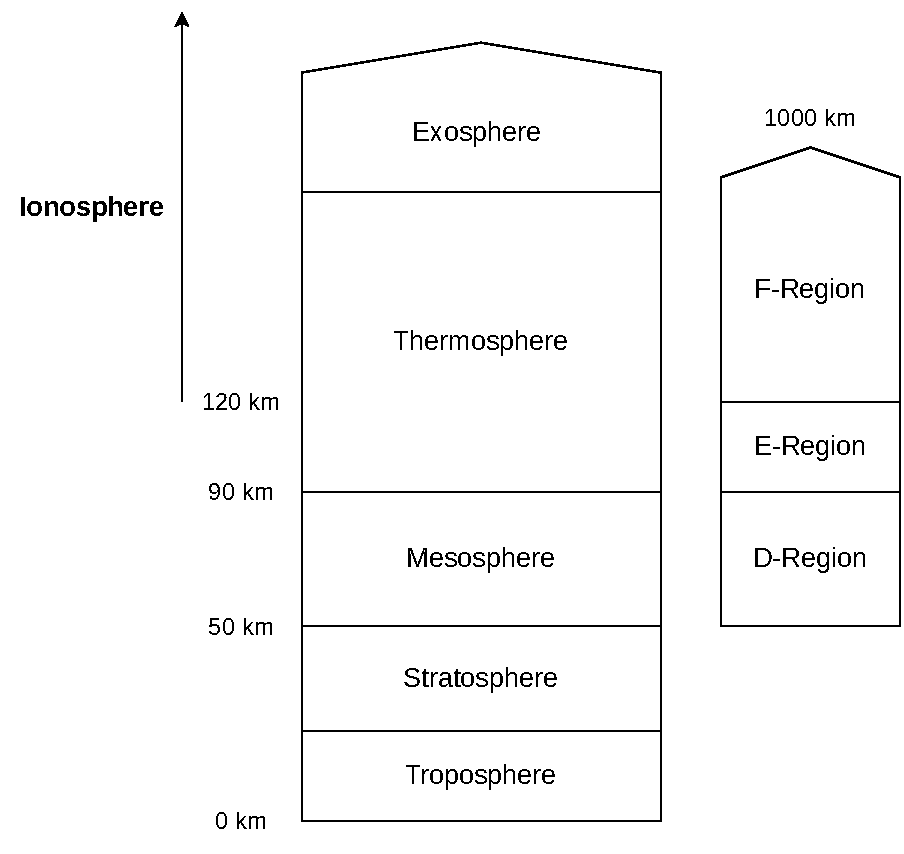
\includegraphics[width=0.6\columnwidth]{figures/atmosphere-model.pdf}
        \caption{Atmosphere model (adapterd from \cite{geog862}).}
        \label{fig:atmosphere-model}
    \end{center}
\end{figure}

% #############################################################################
% #############################################################################
% #############################################################################
% #############################################################################

\section{Telecommunication analysis} \label{sec:telecom-analysis-method}

%Outro aspecto de vital importância para o funcionamento de redes de GNSS está relacionado ao enlace de comunicação entre o satélite e um receptor em terra. Considerando que um satélite de uma rede deste tipo operar em uma altitude de centenas de quilômetros ou até mesmo na faixa dos milhares de quilômetros, a potência do sinal recebido por um receptor em solo é baixa. Para o correto funcionamento do enlace, a potência transmitida, a modulação e os possíveis protocolos envolvidos devem ser compatíveis. Nesta seção apresenta-se os cálculos relacionados ao link budget. O procedimento aqui adotado é o mesmo apresentado em \cite{larson2005}.

Another aspect of vital importance for the functioning of GNSS networks is related to the communication link between the satellite and a ground receiver. Considering that a satellite in such a network operates at an altitude of hundreds or even thousands of kilometers, the power of the signal received by a ground receiver is low. For the link to work correctly, the transmitted power, modulation, and possible protocols involved must be compatible. This section presents the calculations related to the link budget. The procedure adopted here is the same as presented in \cite{larson2005}.

\subsection{Distance to satellite at horizon}

First, the distance between the satellite and a potential receiver must be determined. This distance varies according to the altitude of the satellite and its elevation along the orbit. This way, the distance to satellite at horizon (the maximum theoretical distance between the satellite and a receiver on Earth) can be calculated using \autoref{eq:horizon-distance}.

\begin{equation} \label{eq:horizon-distance}
d = \sqrt{2\cdot R_{e}\cdot h + h^{2}}
\end{equation}

Where:

\begin{itemize}
    \item $R_{e}$ = Earth radius $\cong$ 6378 km
    \item $h$ = Satellite altitude
    \item $d$ = Distance to sattellite at horizon
\end{itemize}

\subsection{Free-Space Path Loss}

The free-space path loss ($FSPL$\nomenclature{\textbf{FSPL}}{Free-Space Path Loss.}) can be calculated using \autoref{eq:fspl}.

\begin{equation} \label{eq:fspl}
FSPL = \left( \frac{4\pi d f}{c} \right)^{2}
\end{equation}

Where:

\begin{itemize}
    \item $d$ = Distance between the satellite and the receiver
    \item $f$ = Radio frequency
    \item $c$ = Speed of light
\end{itemize}

The FSPL value in decibels can be calculated with \autoref{eq:fsbl-db}.

\begin{equation} \label{eq:fsbl-db}
    \begin{split}
        FSPL^{dB} & = 20 \cdot \log\left(\frac{4\pi}{c}\right) + 20 \cdot \log\left(d\right) + 20 \cdot \log\left(f\right) \\
                  & = 32,45 + 20 \cdot \log\left(\frac{d^{km}}{1\ km}\right) + 20 \cdot \log\left(\frac{f^{MHz}}{1\ MHz}\right) \\
    \end{split}
\end{equation}

The minimum distance between the satellite and a receiver is the satellite altitude. The maximum distance is the distance at horizon, defined by \autoref{eq:horizon-distance}.

\subsection{Power at receiver}

The power of the signal at the receiver can be estimated using \autoref{eq:power-at-receiver}.

\begin{equation} \label{eq:power-at-receiver}
    P_{r} = P_{t} + G_{t} + G_{r} - L_{p} - L_{s}
\end{equation}

Where:

\begin{itemize}
    \item $P_{r}$ = Power at the receiver
    \item $P_{t}$ = Transmitter power
    \item $G_{t}$ = Antenna gain of the transmitter
    \item $G_{r}$ = Antenna gain of the receiver
    \item $L_{p}$ = FSPL (Free-Space Path Loss)
    \item $L_{s}$ = Other losses in the system
\end{itemize}

\subsection{Signal-to-Noise-Ratio}

The Signal-to-Noise-Ratio (SNR\nomenclature{\textbf{SNR}}{Signal-to-Noise-Ratio.}) of a transmitted signal at the receiver can be expressed using \autoref{eq:snr}.

\begin{equation} \label{eq:snr}
    SNR = \frac{E_{b}}{N_{0}} = \frac{P_{t}G_{t}G_{r}}{kT_{s}RL_{p}}
\end{equation}

Where:

\begin{itemize}
    \item $P_{t}$ = Transmitter power
    \item $G_{t}$ = Antenna gain of the transmitter
    \item $G_{r}$ = Receiver gain
    \item $k$ = Boltzmann's constant ($\cong 1,3806 \times 10^{-23}\ J/K$)
    \item $T_{s}$ = System noise temperature
    \item $R$ = Data rate in bits per seconds (bps)
    \item $L_{p}$ = Free-Space Path Loss (FSPL)
\end{itemize}

The system noise temperature ($T_{s}$) can be defined using \autoref{eq:system-noise-temperature}.

\begin{equation} \label{eq:system-noise-temperature}
    T_{s} = T_{ant} + T_{r}
\end{equation}

with:

\begin{equation} \label{eq:noise-temperature-receiver}
    T_{r} = \frac{T_{0}}{L_{r}} (F - L_{r})
\end{equation}

and:

\begin{equation} \label{eq:noise-figure}
    F = 1 + \frac{T_{r}}{T_{0}}
\end{equation}

Combining Equations \ref{eq:system-noise-temperature}, \ref{eq:noise-temperature-receiver} and \ref{eq:noise-figure}:

\begin{equation} \label{eq:system-noise-temp-expanded}
    T_{s} = T_{ant} + \left( \frac{T_{0}(1 - L_{r})}{L_{r}} \right) + \left( \frac{T_{0} (F - 1)}{L_{r}} \right)
\end{equation}

Where:

\begin{itemize}
    \item $T_{ant}$ = Antenna noise temperature
    \item $T_{0}$ = Reference temperature (usually 290 K)
    \item $L_{r}$ = Line loss between the antenna and the receiver
    \item $F$ = Noise figure of the receiver
    \item $T_{r}$ = Noise temperature of the receiver
\end{itemize}

The SNR value in decibels can be calculated using the \autoref{eq:snr-db}:

\begin{equation} \label{eq:snr-db}
    \begin{split}
        SNR^{dB} & = 10 \cdot \log_{10}\left( \frac{E_{b}}{N_{0}} \right) = 10 \cdot \log_{10} \left( \frac{P_{t}G_{t}G_{r}}{kT_{s}RL_{p}} \right) \\
                 & = P_{t}^{dBm} - 30 + G_{t}^{dB} + G_{r}^{dB} - L_{p}^{dB} - 10 \cdot \log k - 10 \cdot \log T_{s} - 10 \cdot \log R
    \end{split}
\end{equation}

Considering other losses in the system ($L_{s}$) (cable and connection losses as example), the \autoref{eq:snr-db} can be corrected as presented in \autoref{eq:snr-db-with-losses}.

\begin{equation} \label{eq:snr-db-with-losses}
    SNR^{dB} = P_{t}^{dBm} - 30 + G_{t}^{dB} + G_{r}^{dB} - L_{p}^{dB} - L_{s}^{dB} - 10 \cdot \log k - 10 \cdot \log T_{s} - 10 \cdot \log R
\end{equation}

\subsection{Link margin}

From \cite{larson2005}, the minimum SNR value at the received considering a $10^{-5}$ bit error rate for several type of modulation and coding schemes is available in \autoref{tab:link-margins}.

\begin{table}[!ht]
    \centering
    \begin{tabular}{lC{0.2\textwidth}C{0.2\textwidth}}
        \toprule[1.5pt]
        \textbf{Modulation} & \textbf{$\mathbf{E_{b}/N_{0}}$ for BER = $\mathbf{10^{-5}}$ [dB]} & \textbf{Spectrum utilization} \\
        \midrule
        BPSK                            & 9.6  & 1.0 \\
        DPSK                            & 10.3 & 1.0 \\
        QPSK                            & 9.6  & 2.0 \\
        FSK                             & 13.3 & 0.5 \\
        8FSK                            & 9.2  & 0.375 \\
        BPSK and QPSK $+$ R-1/2 Viterbi & 4.4  & 0.5 and 1.0 \\
        BPSK $+$ RS Viterbi             & 2.7  & 0.44 \\
        MSK                             & 9.6  & 1.5 \\
        \bottomrule[1.5pt]
    \end{tabular}
    \caption{Minimum link margins for several modulation and coding schemes (adapted from \cite{larson2005}).}
    \label{tab:link-margins}
\end{table}

So, the link margin can be obtained by the difference between the SNR and the respective $E_{b}/N_{0}$ value for the communication scheme.

% #############################################################################
% #############################################################################
% #############################################################################
% #############################################################################

\section{Power consumption analysis}

%Um dos aspectos de vital importância nos satélites em geral é a relação entre o consumo e a geração de energia. Especialmente em pequenos satélites, esse aspecto se torna ainda mais relevante e requer ainda mais atenção, devido principalmente ao tamanho reduzido e consequentemente menor capacidade de geração de energia (um volume menor leva a uma menor área disponível para painéis solares).

%Desta forma, uma das principais análises a ser feita para o projeto de uma missão espacial é o power budget, com o objetivo de garantir uma margem positiva de energia ao longo de toda vida útil do satélite.

One of the crucial aspects in satellites in general is the relationship between power consumption and energy generation. Especially in small satellites, this aspect becomes even more relevant and requires even more attention, mainly due to the reduced size and consequently lower energy generation capacity (a smaller volume leads to a smaller area available for solar panels).

Thus, one of the main analyses to be performed for the design of a space mission is the power budget, with the aim of ensuring a positive energy margin throughout the entire useful life of the satellite.

According to section 10.3 of \cite{larson2005}, the power budget of satellite can be determined through three steps:

\begin{enumerate}
    \item Prepare operating power budget
    \item Size the battery
    \item Estimate power degradation over mission life
\end{enumerate}

\subsection{Input power}

%A potência de entrada é o quanto o satélite gera de energia através de seus painéis solares em média ao longo de uma órbita. Dependendo do tipo de órbita, quando o satélite está do lado da Terra em que o Sol está incidindo, há captação de energia solar e armazenamento da mesma nas baterias internas. Nesta fase, o balanço de energia deve ser positivo. Já durante o período em que o satélite está no lado escuro da Terra, praticamente não há captação de energia solar e o balanço de energia torna-se negativo. Levando em conta as duas fases, para o correto funcionamento e durabilidade da missão, o balanço de energia geral ao longo de uma órbita de ser positivo.

%Para se estimar o quanto de energia o satélite irá captar, vários aspectos devem ser levados em conta, como:

%\begin{itemize}
%    \item Tipo de painel solar utilizado (eficiência do mesmo)
%    \item Área dos painéis solares (total e em cada face)
%    \item Geometria do satélite e consequentemente dos painéis solares instalados
%    \item Atitude do satélite ao longo das órbitas
%\end{itemize}

%Para este trabalho, será utilizado o método apresentado em \cite{rigo2023} para se estimar a potência média gerado pelo satélite ao longo de uma órbita para uma determinada configuração e operação do mesmo.

%Por exemplo, para as condições abaixo, tem-se como resultado a curva de geração de energia da \autoref{fig:simulation-input-power-example}.

The input power is how much energy the satellite generates through its solar panels on average throughout an orbit. Depending on the type of orbit, when the satellite is on the side of the Earth where the Sun is shining, there is solar energy capture and storage in the internal batteries. At this stage, the energy balance must be positive. During the period when the satellite is on the dark side of the Earth, there is practically no solar energy capture, and the energy balance becomes negative. Taking into account both phases, for the correct operation and durability of the mission, the overall energy balance over an orbit must be positive.

To estimate how much energy the satellite will capture, several aspects must be taken into account, such as:

\begin{itemize}
    \item Type of solar panel used (its efficiency)
    \item Area of the solar panels (total and on each face)
    \item Geometry of the satellite and therefore the installed solar panels
    \item Attitude of the satellite throughout the orbits
\end{itemize}

For this work, the method presented in \cite{rigo2023} will be used to estimate the average power generated by the satellite over an orbit for a given configuration and operation of the satellite.

For example, for the conditions below, the energy generation curve in \autoref{fig:simulation-input-power-example} is obtained.

\begin{itemize}
    \item Solar irradiance: 1367 $W/m^{2}$
    \item Solar cells efficiency: 30 \%
    \item Total solar cell area: 0.01 $m^{2}$
    \item Timestep: 10 sec
    \item Orbit: Polar with 90$^{\circ}$ of inclination and 550 km of altitude
\end{itemize}

\begin{figure}[!ht]
    \begin{center}
        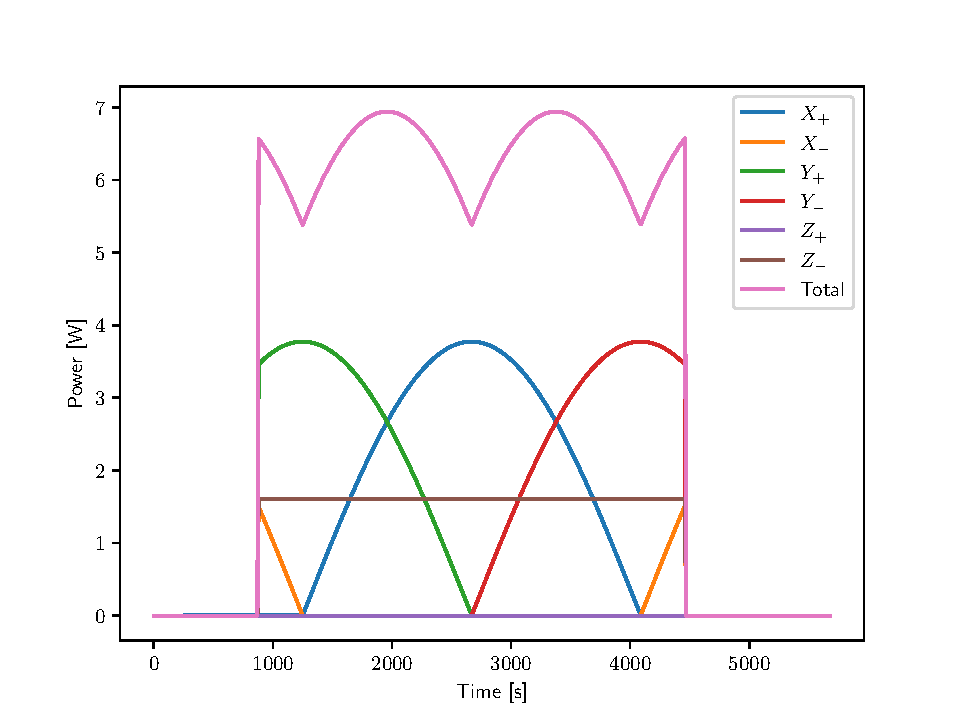
\includegraphics[width=0.9\textwidth]{figures/sim-input-power-3u}
        \caption{Simulated input power of the solar panels using the work of \cite{rigo2023}.}
        \label{fig:simulation-input-power-example}
    \end{center}
\end{figure}

\subsection{Operating power budget}

%Para se obter o orçamento de energia do satélite, precisa-se obter ou estimar os consumos de energia de cada subsistema, juntamente com o quanto cada um ficará ligado durante a operação do mesmo (ou considerar diferentes modos de operação com diferentes consumos para cada subsistema se for o caso).

%Para isso, deve-se ter primeiramente ter os valores de consumo de cada elemento do satélite, e a partir do conceito de operações (CONOPS) definir quanto tempo cada um ficará ligado, na forma de porcentagem em relação ao período de órbita (duty cycle).

To obtain the power budget of the satellite, it is necessary to obtain or estimate the power consumption of each subsystem, along with how long each will be powered on during its operation (or consider different operating modes with different consumption levels for each subsystem if applicable).

To do this, you must first have the power consumption values for each element of the satellite, and based on the concept of operations (CONOPS\nomenclature{\textbf{CONOPS}}{Concept of Operations.}), define how long each will be powered on, in the form of a percentage relative to the orbital period (duty cycle).

Um exemplo pode ser visto na \autoref{tab:power-budget-golds-ufsc}, onde tem-se o power budget previsto para o nanossatélite GOLDS-UFSC \cite{spacelab2022}.

\begin{table}[!ht]
    \centering
    \begin{tabular}{lccccc}
        \toprule[1.5pt]
        \textbf{Module} & \textbf{Duty Cycle [\%]}    & \textbf{Power [mW]} \\
        \midrule
        OBDH                    & 100   & 115 \\
        TTC (radio 1 RX)        & 95    & 65 \\
        TTC (radio 1 TX)        & 5     & 3250 \\
        TTC (radio 2 RX)        & 95    & 65 \\
        TTC (radio 2 TX)        & 5     & 3250 \\
        EPS                     & 100   & 320 \\
        BAT (idle)              & 90    & 0 \\
        BAT (heater full)       & 10    & 5000 \\
        Antenna (deployment)    & 0     & 1800 \\
        Antenna (deployed)      & 100   & 35 \\
        Payload EDC             & 100   & 1250 \\
        Radiation instrument    & 0     & 1000 \\
        \cmidrule{2-3}
        Satellite               & \multicolumn{2}{c}{$\cong$ 2668 mW} \\
        \bottomrule[1.5pt]
    \end{tabular}
    \caption{Power consumption of the subsystems and payloads of the nanosatellite GOLDS-UFSC.}
    \label{tab:power-budget-golds-ufsc}
\end{table}

By utilizing the mean power consumption of the satellite and the mean power generation per orbit, we can achieve power balance within one orbit. If the satellite has more than one mode of operation, this process must be carried out for each mode.

%Para um correto dimensionamento energético, a degradação dos elementos de geração de energia, como os painéis solares, deve ser levada em conta. Dessa forma, para garantir um balanço de energia positivo ao longo de toda vida útil do satélite, deve-se garantir a queda na captação e geração de energia ao final da vida útil. 

For accurate energy sizing, the degradation of energy generation elements, such as solar panels, must be taken into account. Therefore, to ensure a positive energy balance throughout the satellite's entire lifespan, a decrease in energy capture and generation at the end of its life must be guaranteed. From \cite{larson2005}, 5 \% per year is a usual number for the solar panels’ degradation, in other words, the general efficiency of the solar panels decays at a rate of 5 \% per year of operation.

%Com os valores de geração de energia e consumo definidos, o próximo passo é o dimensionamento da bateria do satélite, que armazena energia quando o mesmo está captando energia solar, e fornece energia para toda a eletrônica quando o satélite está em um momento de eclipse. Do mesmo modo, o balanço de energia deve se manter positivo entre as fases de carga e descarga das baterias, ou seja, deve-se garantir que o consumo de energia durante a descarga seja menor que a entrada de energia durante a carga. Dependendo da tecnologia utilizada, também deve-se garantir alguns aspectos de operação, como por exemplo um valor de carga mínimo armazenada na bateria e uma temperatura de operação adequada. E da mesma forma que os painéis solares, também deve se considerar a degradação da mesma ao longo da vida útil do satélite. Normalmente considera-se uma uma taxa de perda de armazenamento de 10 \% ao ano.

With the defined values of energy generation and consumption, the next step is the sizing of the satellite's battery, which stores energy when the satellite is capturing solar energy and supplies power to all electronics during eclipse periods. Similarly, the energy balance must remain positive between the charging and discharging phases of the batteries. This means that the energy consumption during discharge should be lower than the energy input during charging. Depending on the technology used, certain operational aspects must also be ensured, such as a minimum charge value stored in the battery and an appropriate operating temperature. Additionally, like solar panels, the battery's degradation over the satellite's lifespan must also be taken into consideration. Typically, a storage loss rate of 10 \% per year is considered\footnote{The capacity degradation rate of the batteries depends on a lot of variables, like temperature variation, the number of charge and discharge cycles, and so on.}.

% #############################################################################
% #############################################################################
% #############################################################################
% #############################################################################

\section{Orbit analysis}

%Por fim, uma análise também de extrema importância para um correto projeto e dimensionamento de um satélite é a análise de órbita. A órbita em que o satélite irá operar influência por exemplo nos canais de comunicação e na geração de energia. Além disso, está diretamente relacionada com o propósito e o plano de operação do satélite, determinando muitas vezes por quanto tempo o satélite permanecerá em operação.

%Para um satélite com o objetivo de transmitir sinais de geolocalização para qualquer região do planeta, deseja-se que o mesmo tenha uma cobertura a nível global e que consiga transmitir os seus sinais para qualquer região do globo. Desta forma, a órbita escolhida deve levar este ponto em consideração. No caso deste trabalho, umas das possibilidades é a da utilização de órbitas baixas, um tipo de órbita que se adequá nesse requisito são as órbitas polares, com um ângulo de inclinação próximo dos 90$^{\circ}$.

%Para o caso de sistemas regionais, outros tipos de órbitas podem ser levadas em consideração, como por exemplo elevações mais baixas e/ou diferentes valores de apogeu e perigeu, para cobrir só uma faixa ou região específica do globo.

%Para realizar esse tipo de análise, normalmente se recorre a software de simulações de órbita. Há diversas aplicações disponíveis atualmente, mas entre as mais usadas por se destacar o STK \cite{STK} e o FreeFlyer \cite{freeflyer}, que são ferramentas comerciais, e o GMAT \cite{gmat} que é uma ferramenta aberta.

Finally, an analysis of utmost importance for the correct design and sizing of a satellite is the orbit analysis. The orbit in which the satellite will operate influences, for example, the communication channels and power generation. Moreover, it is directly related to the purpose and operational plan of the satellite, often determining how long the satellite will remain in operation.

For a satellite aiming to transmit geolocation signals to any region of the planet, it is desired to have global coverage and be able to transmit its signals to any part of the globe. Therefore, the chosen orbit must take this into consideration. In the case of this work, one possibility is the use of low orbits, specifically polar orbits with an inclination angle close to 90 degrees, as they are suitable for meeting this requirement.

For regional systems, other types of orbits can be considered, such as lower elevations and/or different values of apogee and perigee, to cover only a specific range or region of the globe.

To perform this type of analysis, orbit simulation software is commonly used. There are several applications available today, but among the most widely used are the commercial tools STK\nomenclature{\textbf{STK}}{System Took Kit.} (Systems Tool Kit) \cite{STK} and FreeFlyer \cite{freeflyer}, as well as the open-source tool GMAT\nomenclature{\textbf{GMAT}}{General Mission Analysis Tool.} (General Mission Analysis Tool) \cite{gmat}.
    %
% proposed-work.tex
%
% Copyright (C) 2022 by Universidade Federal de Santa Catarina.
%
% GNSS Networks Based on Small Satellites
%
% This work is licensed under the Creative Commons Attribution-ShareAlike 4.0
% International License. To view a copy of this license,
% visit http://creativecommons.org/licenses/by-sa/4.0/.
%

%
% \brief Proposed work chapter.
%
% \author Gabriel Mariano Marcelino <gabriel.mm8@gmail.com>
%
% \version 0.1.0
%
% \date 2021/06/14
%


\chapter{Proposed Work} \label{ch:proposed-work}

%Neste capítulo apresenta-se o trabalho proposto por essa tese. Que resumidamente consiste no estudo da viabilidade da implantação de redes de GNSS utilizando satélites de pequeno porte, podendo operar tanto em órbitas convencionais para este tipo de aplicação, mas principalmente em órbitas baixas, em altitudes que vêm sendo mais exploradas atualmente por esses tipos de dispositivos.

In this chapter, we present the work proposed by this thesis. Briefly, it consists of the study of the feasibility of implementing GNSS networks using small satellites, which can operate in both conventional orbits for this type of application, but mainly in low orbits, at altitudes that are currently being more explored by these types of devices.

\section{Orbit study}

%Além da proposta principal deste trabalho da utilização de pequenos satélites para a implantação de uma rede de GNSS, também tem-se como discussão a utilização de órbitas mais baixas para esse tipo de sistema. Atualmente as redes de GNSS já em operação trabalham em órbitas médias (MEO), na faixa dos 20000 km de altitude. Neste tipo de órbita as condições ambientais são extremamente nocivas para os subsistemas de um satélite, especialmente os componentes eletrônicos, que são submetidos a altas doses de radiação e temperaturas extremas, que provocam danos aos mesmos, diminuindo consideravelmente a sua vida útil, ou até mesmo danificando-o permanentemente.

%Para permitir a operação dos satélites neste tipo de órbita, são utilizados componentes com um certo nível de tolerância a radiação, que aguentam certas doses da mesma e permitem um maior tempo de vida. Mas esses tipos de componentes possuem um alto custo e são de difícil acesso, devido principalmente a restrições de fornecimento por parte dos países que o produzem (regulações do tipo ITAR por exemplo). Além de questões ligadas a radiação incindindo nos componentes, também há problemas ligadas a temperatura a que eles são submetidos. Em órbitas médias, temperatura negativas são comuns e requerem o uso de componentes que conseguem operar neste tipo de ambiente, como por exemplo componentes com especificações automotivas (-40 à 125 $^{\circ}$C) ou militares (-55 à 125 $^{\circ}$C). Em certos casos, também há a necessidade da utilização de controle ativo de temperatura, o que requer gasto de energia para manter integridade e/ou correto funcionamento de certos subsistemas ou componentes.

%Com a utilização de órbitas baixas (LEO), alguns desses problemas são atenuados. Devido a influência do campo magnético da Terra, os níveis de radiação em órbitas LEO são menores quando comparados com órbitas MEO. Neste caso há requisitos de tolerância menores, fazendo com que se possa utilizar componentes mais simples ou até mesmo sem classificação rad-hard. Estratégias mecânicas podem ser suficientes para a filtrar ou até mesmo barrar partículas. Além da questão de radiação, o controle térmico também torna-se mais fácil, já que a faixa de temperatura em que os satélites ficam submetidos nessa altitude é menor. Neste, dependendo do subsistema pode não haver a necessidade de um controle de temperatura ativo.

%Outro aspecto que se altera com a redução da altitude de operação, é em relação ao link de comunicação, mas especificamente o próprio sinal de GNSS gerado e transmitido pelos satélites. Como em uma órbita mais baixa, a distância entre o transmissor e um recepto em terra torna-se menor, a potência do sinal transmitido também pode ser reduzida. Desta forma, transmissores mais simples podem ser utilizados, e o consumo de energia também torna-se menor, fazendo com que no geral o satélite também possa ser reduzido fisicamente.

%E por fim, outro aspecto que se altera reduzindo a órbita de operação, é em relação ao número de satélites necessários para se ter uma cobertura total de uma certa região ou até mesmo a nível global. Neste caso, a utilização de uma órbita mais baixa trás uma desvantagem, já que são necessários mais satélites em relação a mesma situação em uma órbita do tipo MEO. Além de uma menor área de visada quando se trabalha com satélites mais baixos, o tempo de visada também torna-se menor. Neste cenário, o número de satélites necessários torna-se consideravelmente maior. Um exemplo dessa situação pode ser visto na \autoref{fig:footprint-comparison}, onde tem-se a área de visada de um satélite da rede GPS à uma altitude de aproximadamente 20000 km à esquerda, e de a área de visada de um CubeSat em órbita uma órbita de aproximadamente 600 km à direita. 

In addition to the main proposal of this work on the use of small satellites for the implementation of a GNSS network, the use of lower orbits for this type of system is also discussed. Currently, operational GNSS networks operate in medium orbits (MEO), at around 20,000 km altitude. In this type of orbit, environmental conditions are extremely harmful to satellite subsystems, especially electronic components, which are subjected to high doses of radiation and extreme temperatures that cause damage, significantly reducing their lifespan, or even permanently damaging them.

To allow satellite operation in this type of orbit, radiation-tolerant components are used, which can withstand certain doses of radiation and allow for longer lifespan. However, these types of components are expensive and difficult to obtain, mainly due to supply restrictions from countries that produce them (such as ITAR regulations). In addition to radiation-related issues affecting components, there are also temperature-related issues. In medium orbits, negative temperatures are common and require the use of components that can operate in such an environment, such as components with automotive (-40 to 125 $^{\circ}$C) or military (-55 to 125 $^{\circ}$C) specifications. In some cases, active temperature control is also required, which requires energy expenditure to maintain the integrity and/or proper functioning of certain subsystems or components.

With the use of low Earth orbits (LEO), some of these problems are mitigated. Due to the influence of the Earth's magnetic field, radiation levels in LEO are lower compared to MEO orbits. In this case, there are lower tolerance requirements, making it possible to use simpler or even non-rad-hard classified components. Mechanical strategies can be sufficient to filter or even block particles. In addition to radiation issues, thermal control also becomes easier, as the temperature range in which satellites are subjected at this altitude is smaller. In this case, depending on the subsystem, there may be no need for active temperature control.

Another aspect that changes with the reduction in operating altitude is related to the communication link, specifically the GNSS signal generated and transmitted by the satellites themselves. As the distance between the transmitter and a ground receiver becomes shorter in a lower orbit, the power of the transmitted signal can also be reduced. Thus, simpler transmitters can be used, and energy consumption also becomes lower, allowing the satellite to be physically reduced overall.

Finally, another aspect that changes by reducing the operating orbit is related to the number of satellites required to achieve full coverage of a certain region or even globally. In this case, the use of a lower orbit brings a disadvantage, as more satellites are required compared to the same situation in a MEO orbit. In addition to a smaller line-of-sight area when working with lower satellites, the line-of-sight time also becomes shorter. In this scenario, the number of required satellites becomes considerably higher. An example of this situation can be seen in \autoref{fig:footprint-comparison}, where the line-of-sight area of a GPS network satellite at an altitude of approximately 20,000 km is shown on the left, and the line-of-sight area of a CubeSat in orbit at an altitude of approximately 600 km is shown on the right.

\begin{figure}[!htb]
    \begin{center}
        \subfigure[Footprint of a GPS satellite, GPS BIIR-5 (PRN 28).\label{fig:footprint-gps}]
        {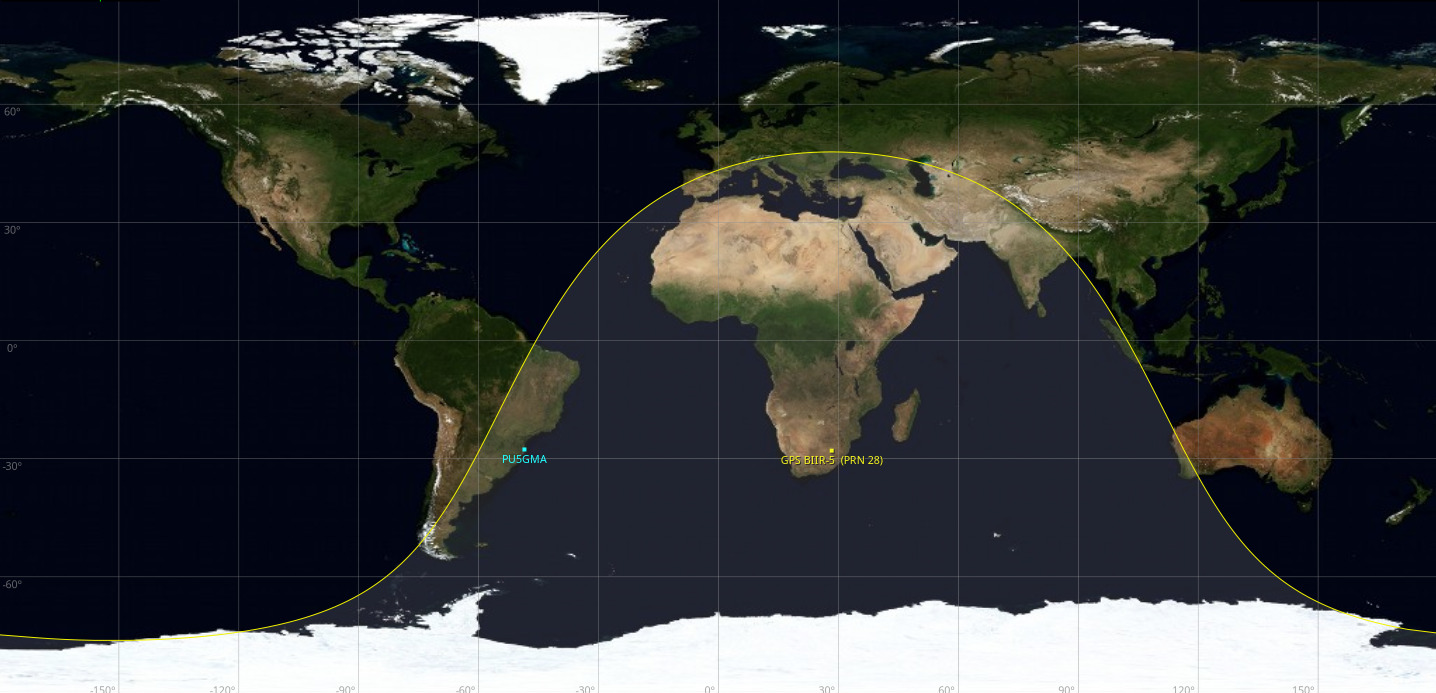
\includegraphics[width=\textwidth]{figures/footprint-gps.jpg}}
        ~
        \subfigure[Footprint of a LEO CubeSat, ITASat-1.\label{fig:footprint-itasat}]
        {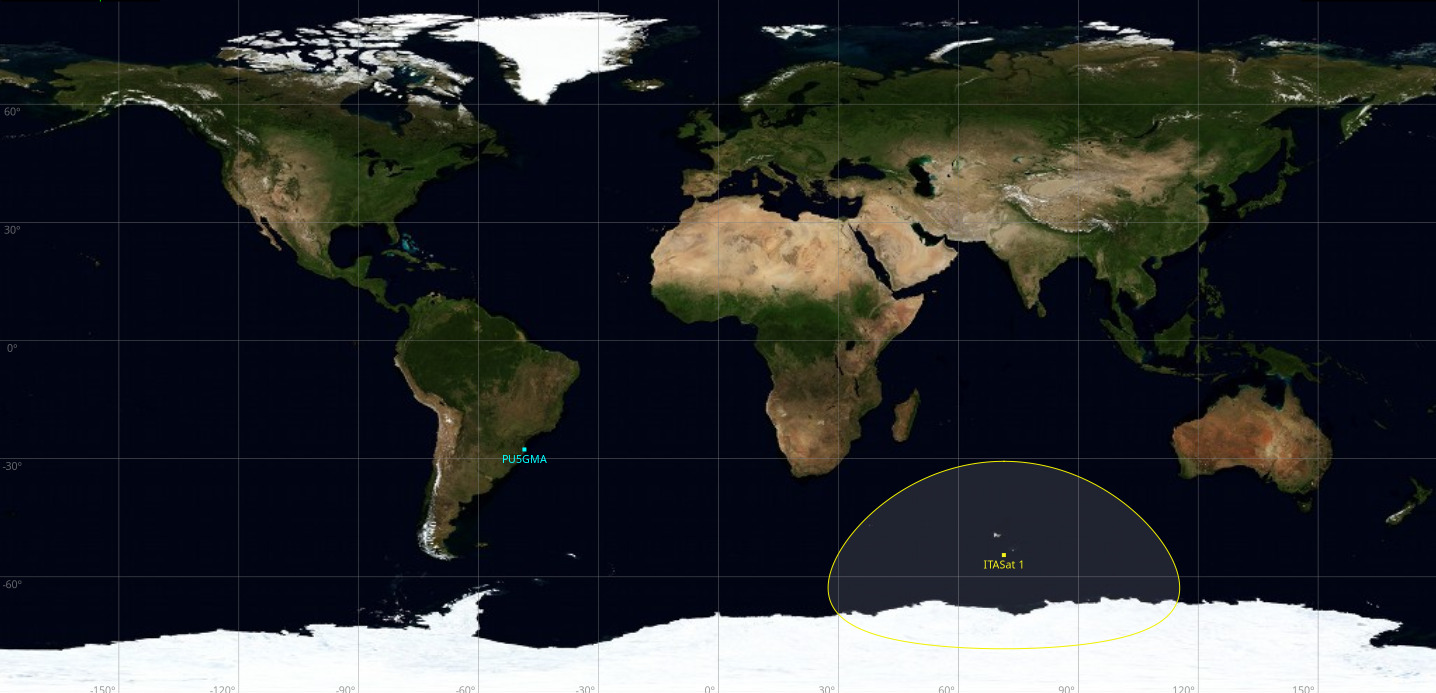
\includegraphics[width=\textwidth]{figures/footprint-itasat.jpg}}
        \caption{Comparison of the footprint area of a satellite in MEO orbit and one in a LEO orbit.}
        \label{fig:footprint-comparison}
    \end{center}
\end{figure}

\subsection{Preliminary simulations}

%Como primeiras análises de órbita, tendo como objetivo determinar principalmente o tempo de decaimento, o período para uma volta e a quantidade necessária de satélites, nesta seção apresenta-se as primeiras simulações de órbita realizadas. Para isso, utilizou-se o software GMAT, tendo como referência uma TLE do nanossatélite FloripaSat-1 \cite{marcelino2021} (modificada para uma altitude mais baixa), juntamente com os modelos de órbita e parâmetros utilizados em \cite{marino2016}. Os parâmetros de órbita adotados podem ser vistos na \autoref{tab:orbit-parameters}.

As initial orbit analyses, aiming to determine primarily the decay time, the period for one revolution, and the required quantity of satellites, this section presents the first orbit simulations conducted. For this purpose, the GMAT software was used, taking as reference a TLE of the FloripaSat-1 nanosatellite \cite{marcelino2021} (modified for a lower altitude), along with the orbit models and parameters used in \cite{marino2016}. The adopted orbit parameters can be seen in \autoref{tab:orbit-parameters}.

%To define the orbit parameters and simulate the behaviour of the satellite during its operation, the GMAT software was used \cite{gmat}. The orbit parameters was based on the FloripaSat-I TLE, but with a lower altitude. These parameters can be seen in \autoref{tab:orbit-parameters}.

\begin{table}[!ht]
    \centering
    \begin{tabular}{lcc}
        \toprule[1.5pt]
        \textbf{Parameters} & \textbf{Value} & \textbf{Unit} \\
        \midrule
        Altitude                & 550           & km \\
        Eccentricity            & 0,0015051     & $^{\circ}$ \\
        Inclination             & 97,9750       & $^{\circ}$ \\
        RAAN                    & 85,5100       & $^{\circ}$ \\
        Arg. of Perigee (AOP)   & 194,87        & $^{\circ}$ \\
        TA                      & 99,8877       & $^{\circ}$ \\
        \bottomrule[1.5pt]
    \end{tabular}
    \caption{Initial orbit parameters (adapted from FloripaSat-1).}
    \label{tab:orbit-parameters}
\end{table}

The parameters of the orbit model used in the GMAT simulation (based on the work of \cite{marino2016}) can be seen listed below:

\begin{itemize}
    \item Force model for gravitational field: ``\textit{Earth Gravitational Model 1996 (EGM96)}'' \cite{lemoine1998}
    \item Propagator: ``\textit{PrinceDorman78}''
    \item Drag coefficient: 2,2
    \item Drag atmosphere model: ``\textit{Mass Spectrometry and Incoherent Scatter (MSISE90)}'' \cite{hedin1991}
    \item Epoch: 01 Jan 2022 11:59:28.000
\end{itemize}

%Executando-se essa simulação por um período de algumas horas, chegou-se aos resultados da Figuras \ref{fig:fsat2-gmat} e \ref{fig:fsat2-gmat-groundtrack}.

Running this simulation for a few hours, the results shown in Figures \ref{fig:fsat2-gmat} and \ref{fig:fsat2-gmat-groundtrack} were obtained. The \autoref{fig:fsat2-gmat} shows the 3D representation of the obtained orbit simulation, \autoref{fig:fsat2-gmat-groundtrack} shows the ground track of the first day of operation. As can be seen, and as expected, a polar orbit with global coverage was achieved.

\begin{figure}[!ht]
    \begin{center}
        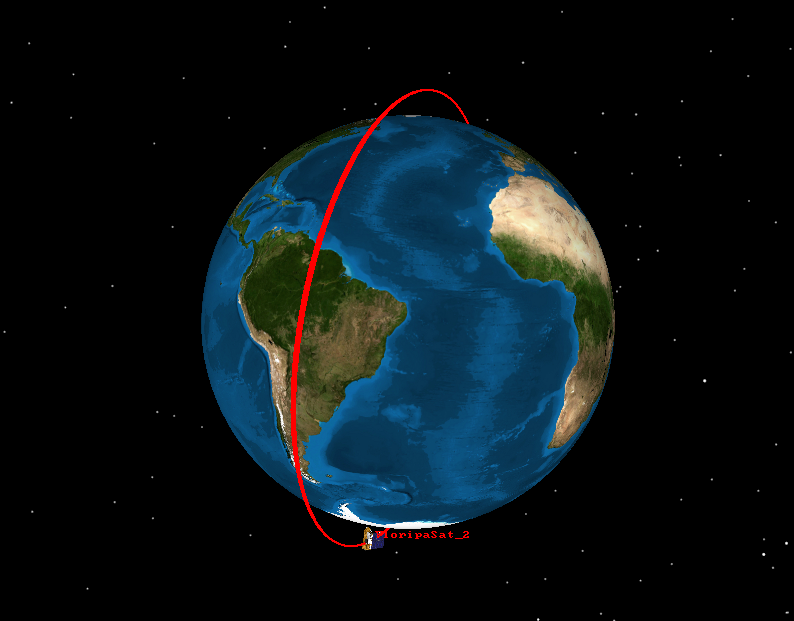
\includegraphics[width=0.6\columnwidth]{figures/fsat2-gmat.png}
        \caption{3D representation of the obtained orbit in the GMAT's simulation.}
        \label{fig:fsat2-gmat}
    \end{center}
\end{figure}

\begin{figure}[!ht]
    \begin{center}
        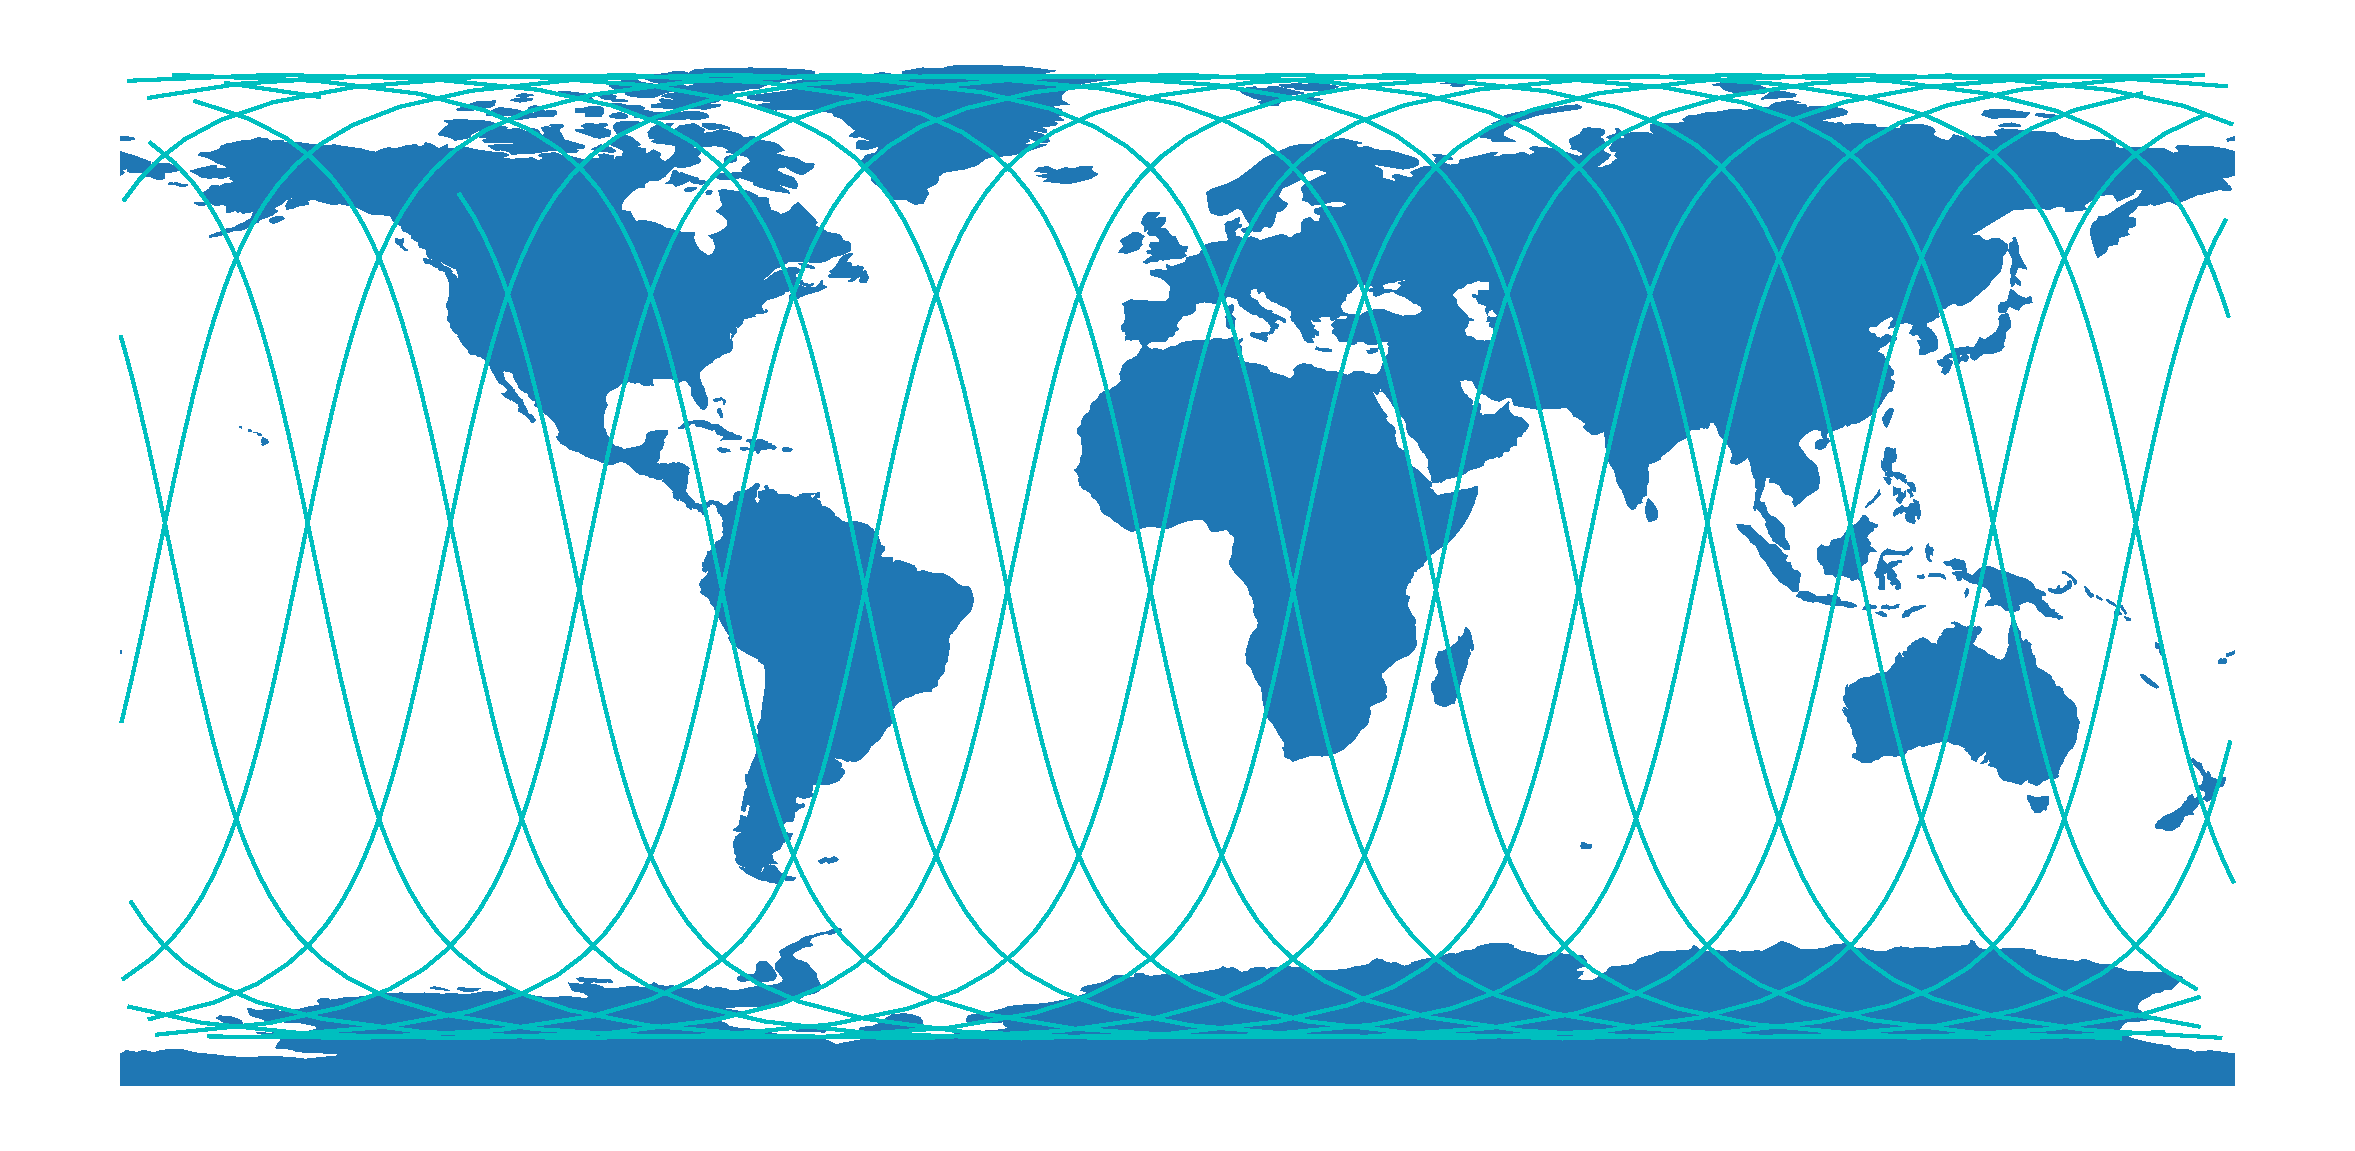
\includegraphics[width=\columnwidth]{figures/fsat2-gmat-groundtrack.pdf}
        \caption{Groundtrack of the obtained simulation.}
        \label{fig:fsat2-gmat-groundtrack}
    \end{center}
\end{figure}

The next section present some analysis based on the results obtained on the simulations executed on GMAT.

%The source files of the GMAT simulation are available in \cite{fsat2-mechanical}.

\subsection{Lifetime analysis}

Considering the same parameters presented above, with an initial altitude of 550 km, the simulations on GMAT showed that the satellite decays approximately in 2000 days ($\cong$ 5 years), as can be seen in \autoref{fig:lifetime-analysis}.

\begin{figure}[!ht]
    \begin{center}
        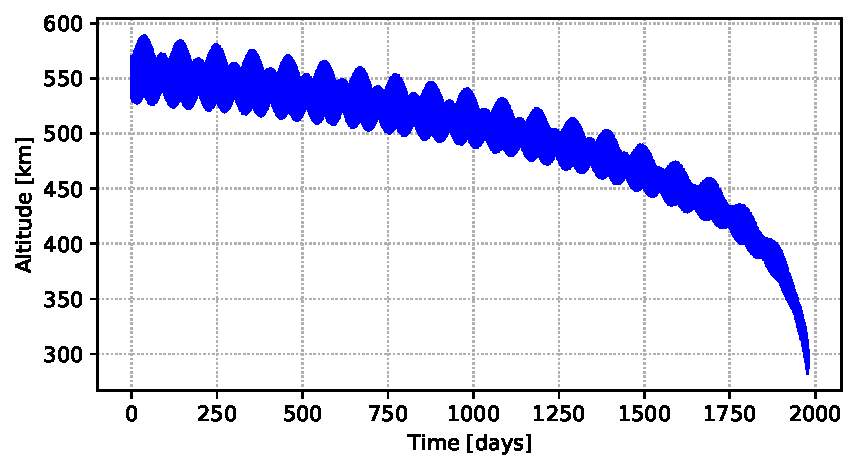
\includegraphics[width=\columnwidth]{curves/lifetime.pdf}
        \caption{Lifetime analysis on GMAT.}
        \label{fig:lifetime-analysis}
    \end{center}
\end{figure}

Lançamentos em órbitas polares e em altitude entre 500 e 600 km sãos os que tem maior disponibilidade atualmente. Sendo portanto, geralmente, os de menor custo e mais frequentes. Como oferece uma cobertura global (ou seja, é possível se comunicar com o satélite em qualquer região do globo), e um bom tempo de decaimento, torna-se ideal para missões de pequenos satélites e de baixo custo.

%Este resultado é apenas preliminar e serve apenas como uma referência. Resultados mais precisos relacionados a órbita e principalmente ao decaimento dependem de mais definições da missão, como por exemplo a data lançamento e o tamanho do satélite.

This result is only preliminary and serves as a reference only. More accurate results related to the orbit and, especially, decay depend on further mission specifications, such as the launch date and the satellite's size.

\section{Communication study}

%Um outro tipo de análise de extrema importância para o planejamento de missões satelitais, e de ainda maior importância tratando-se de um sistema de posicionamento por satélites, é a análise de comunicação. Esta análise tem como objetivo determinar a viabilidade do canal de comunicação entre o satélites e uma estação na Terra.

%Utilizando-se o método e as equações apresentadas em \autoref{sec:telecom-analysis-method}, chega-se aos resultados abaixo.

Another type of analysis of extreme importance for satellite mission planning, and of even greater importance for a satellite positioning system, is the communication analysis. This analysis aims to determine the feasibility of the communication channel between the satellites and a ground station.

By using the method and equations presented in Section \ref{sec:telecom-analysis-method}, the following results are obtained.

Fist, the distance to satellite at horizon can be obtained using \autoref{eq:horizon-distance}. Same way as used in the orbit simulation, considering an altitude of 550 km, the maximum distance between the satellite and an station on Earth, is approximately 2700 km, as can be seen in \autoref{eq:horizon-distance-result}.

\begin{equation} \label{eq:horizon-distance-result}
d = \sqrt{2\cdot 6378\cdot 550 + 550^{2}} = \mathbf{2705\ km}
\end{equation}

Considering a frequency of 900 MHz (one possible frequency band that can be used for the proposed service), the minimum and maximum FSBL is as presented in Equations \ref{eq:fslp-min-result} and \ref{eq:fspl-max-result}.

\begin{equation} \label{eq:fslp-min-result}
    FSPL^{dB}_{min} = 32,45 + 20\log\left(\frac{550}{1\ km}\right) + 20\log\left(\frac{900}{1\ MHz}\right) \cong \mathbf{146.3\ dB}
\end{equation}

\begin{equation} \label{eq:fspl-max-result}
    FSPL^{dB}_{max} = 32,45 + 20\log\left(\frac{2705}{1\ km}\right) + 20\log\left(\frac{900}{1\ MHz}\right) \cong \mathbf{160.2\ dB}
\end{equation}

This way, the FSPL can be will in the following range during a satellite pass:

\begin{equation}
    \mathbf{146.3 \leq FSPL^{dB} \leq 160.2\ dB}
\end{equation}

Considering the worst scenario with the maximum possible distance between the satellite and a receiver on Earth, a transmitter in the satellite with a output power of 30 dBm (1 W), antennas with 3 dBi of gain, and 5 dB as general losses, the power at the receiver for the link is calculated below.

\begin{equation}
    P_{r} = 30 + 3 + 3 - 160.2 - 5 = -129.2\ dBm
\end{equation}

\begin{equation}
    \mathbf{P_{r} \geq -129.2\ dBm}
\end{equation}

For calculating the SNR of the received signal, Equations \ref{eq:snr-db-with-losses} and \ref{eq:system-noise-temperature} can be used, with:

\begin{itemize}
    \item $P_{t} = 30\ dBm$
    \item $G_{t} = 3\ dBi$
    \item $G_{r} = 3\ dBi$
    \item $L_{p} = 160.2\ dB$
    \item $L_{s} = 5\ dB$
    \item $R = 1200\ bps$
    \item $T_{0} = 290\ K$
    \item $T_{r} = 290\ K$
    \item $T_{ant} = 300\ K$
    \item $F = 2\ dB$
    \item $L_{r} = 0,89\ (0,5\ dB)$
\end{itemize}

The results are presented below:

\begin{equation}
    T_{s} = 300 + \left( \frac{290 (1 - 0,89)}{0,89} \right) + \left( \frac{290 (2 - 1)}{0,89} \right) = 661,7\ K
\end{equation}

\begin{equation}
    SNR^{dB} = 30 - 30 + 3 + 3 - 160.2 - 5 + 228.6 - 28.21 - 30.79 = 10.4\ dB
\end{equation}

\begin{equation}
\mathbf{SNR^{dB} \geq 10.4\ dB}
\end{equation}

Considering the link margin as the SNR of the link minus the SNR threshold for a given bit error, the link margin of the radio links of the satellite are:

\begin{itemize}
    \item Resultant link margin: $10.4 - 9.6 = \mathbf{0.8\ dB}$
\end{itemize}

The SNR threshold was taken from \autoref{tab:link-margins}, and is the estimated value considering the BPSK modulation and a BER\nomenclature{\textbf{BER}}{Bit Error Rate.} of $10^{5}$.

As can be seen, the resultant link margin for the considered parameters is low. However, this result considers the worst-case scenario where a zero degree of elevation between the observer and the satellite is assumed. For a more realistic scenario, a higher minimum elevation should be considered. In practice, it is challenging to achieve a clear line of sight without obstacles when the satellite is at the horizon. With a higher elevation, the Free Space Path Loss (FSPL) of the link will be lower, resulting in a higher Signal-to-Noise Ratio (SNR).

Other aspects can also be considered. For example, active antennas with higher gains can be used for the system, especially on the receiver side.

\section{Required power budget}

%Com a ideia aqui proposta para a implementação de um sistema de de GNSS baseado em pequenos satélites, um das principais dificuldades de tal implementação está relacionada a geração de energia de cada satélite da rede. Como satélites de pequeno porte possuem limitações em relação a área dos painéis solares e ao armazenamento de energia, devido ao tamanho reduzido, a energia disponível para o subsistemas do satélite é limitada.

%Sendo assim, nessa seção se analisará os requisitos de energia necessários para tal sistema considerando a utilização de subsistemas comumentemente utilizados em CubeSats e encontrados a venda no mercado, e estimativas de consumo para alguns subsistemas.

%Na \autoref{tab:power-budget-subsystems}, encontram-se os subsistemas considerados para essa análise.

With the idea proposed here for the implementation of a GNSS system based on small satellites, one of the main difficulties of such implementation is related to the power generation for each satellite in the network. Since small satellites have limitations regarding the area of solar panels and energy storage, due to their reduced size, the available energy for the satellite subsystems is limited.

Therefore, in this section, we will analyze the power requirements necessary for such a system, considering the use of subsystems commonly used in CubeSats and available in the market, as well as estimates of power consumption for some subsystems.

In \autoref{tab:power-budget-subsystems}, the subsystems considered for this analysis can be found, with the respective power consumption range.

\begin{table}[!ht]
    \centering
    \begin{tabular}{lcccc}
        \toprule[1.5pt]
        \textbf{Subsystem} & \textbf{Manufacturer} & \textbf{Model} & \textbf{Consumption [mW]} \\
        \midrule
        OBDH     & GomSpace & NanoMind A3200 & 170 \\
        EPS      & GomSpace & NanoPower P60  & 160 \\
        Battery  & GomSpace & NanoPower BP4  & 50-7000 \\
        TMTC     & GomSpace & NanoCom AX100  & 300-3300 \\
        Antenna  & ISISpace & AntS           & 35-1800 \\
        ADCS     & ISISpace & iMTQ           & 175-1200 \\
        GNSS Transmitter & \multicolumn{2}{c}{Custom model} & 4720 \\
        \bottomrule[1.5pt]
    \end{tabular}
    \caption{Power consumptions reference.}
    \label{tab:power-budget-subsystems}
\end{table}

%Para o transmissor de GNSS, conforme apresentado na \autoref{sec:ionospheric-delay}, se considerará dois transmissores operando em tempo integral. Como base para os cálculos, será considerado o consumo de um transmissor operando em Banda-S disponível no mercado e voltado especificamente para CubeSats (modelo NanoCom AX2150, da GomSpace \cite{ax2150}). Este apresenta um consumo de 2200 mW durante a transmissão, e de 500 mW durante o modo de recepção. Já para a parte da referência de tempo, se utilizará como base os valores de consumo do oscilador de rubídio CSAC SA.45S da Microchip. Conforme descrito na documentação do mesmo, este apresenta um consumo de 120 mW durante uma operação normal. Para as antenas dos transmissores, também se considerará o consumo de uma antena para Banda-S disponível comercialmente para CubeSats (modelo NanoCom AM2150-P, da GomSpace \cite{am2150-p}). Neste caso, por tratar-se de uma antena passiva, o consumo considerado será zero. Por fim, para outros possíveis elementos de payload como microcontrolador e sensores, se considerará um consumo de 200 mW. Os valores de consumo considerados para o payload de GNSS estão descritos na \autoref{tab:power-gnss-payload}.

For the GNSS transmitter, as presented in \autoref{sec:ionospheric-delay}, two transmitters operating full-time will be considered. As a basis for the calculations, the power consumption of a commercially available Band-S transmitter specifically designed for CubeSats will be taken into account (NanoCom AX2150 model, from GomSpace \cite{ax2150}). This transmitter has a consumption of 2200 mW during transmission and 500 mW during reception mode. As for the time reference component, the power consumption values of the CSAC SA.45S rubidium oscillator from Microchip will be used as a basis. According to the documentation, this oscillator has a consumption of 120 mW during normal operation. For the transmitter antennas, the power consumption of a commercially available S-Band antenna for CubeSats will also be considered (NanoCom AM2150-P model, from GomSpace \cite{am2150-p}). In this case, as it is a passive antenna, the consumption will be considered as zero. Finally, for other potential payload elements such as microcontrollers and sensors, a consumption of 200 mW will be considered. The power consumption values considered for the GNSS payload are synthetized in \autoref{tab:power-gnss-payload}.

\begin{table}[!ht]
    \centering
    \begin{tabular}{lcccc}
        \toprule[1.5pt]
        \textbf{Item} & \textbf{Quantity} & \textbf{Consumption [mW]} \\
        \midrule
        RF transmitter  & 2 & 2200 \\
        Clock reference & 1 & 120 \\
        Antenna         & 2 & 0 \\
        Others          & 1 & 200 \\
        \cmidrule{2-3}
        Total           & \multicolumn{2}{c}{4720} \\
        \bottomrule[1.5pt]
    \end{tabular}
    \caption{Estimated power consumption of the GNSS payload.}
    \label{tab:power-gnss-payload}
\end{table}

%Para o duty cycle e modos de operação se utilizará como referência o utilizado em outras missões de CubeSat. Neste caso, assume-se os módulos de serviço operando da mesma forma que em um CubeSat em uma missão ``genérica''.

For the duty cycle and operating modes, the reference will be based on those used in other CubeSat missions. In this case, it is assumed that the service modules operate in the same way as in a ``generic'' CubeSat mission, with the TMTC in reception mode most of the time, the ADCS operating just with small attitude corrections and the battery heater activated only during eclipses. The \autoref{tab:power-duty-cycle} presents the power consumptions and respective duty cycles.

\begin{table}[!ht]
    \centering
    \begin{tabular}{lcc}
        \toprule[1.5pt]
        \textbf{Subsystem} & \textbf{Duty Cycle [\%]} & \textbf{Power [mW]} \\
        \midrule
        OBDH                  & 100 & 170 \\
        TMTC (RX)             & 95  & 300 \\
        TMTC (TX)             & 5   & 3300 \\
        EPS                   & 100 & 160 \\
        Battery (idle)        & 90  & 50 \\
        Battery (heater full) & 10  & 7000 \\
        ADCS (idle)           & 90  & 175 \\
        ADCS (full actuation) & 10  & 1200 \\
        Antenna (deployment)  & 0   & 1800 \\
        Antenna (deployed)    & 100 & 35 \\
        Payload GNSS          & 100 & 4720 \\
        \cmidrule{2-3}
        Satellite             & \multicolumn{2}{c}{$\cong$ 6526 mW} \\
        \bottomrule[1.5pt]
    \end{tabular}
    \caption{Power consumption and duty cycle of each subsystem, and average total power of the satellites.}
    \label{tab:power-duty-cycle}
\end{table}

As can be seen from \autoref{tab:power-duty-cycle}, an average power consumption of 6526 mW was achieved for the considered system. This value is highly influenced by the power consumption of the GNSS payload, which is not the highest in the system but has a duty cycle of 100 \%. For a global GNSS system, it is expected that the transmitters are always transmitting the timing data.

With the estimated power consumption, the required area of solar panels can be calculated, and consequently, the minimum size of the satellite can be defined.

Using the method of \cite{rigo2023}, with a solar irradiance of 1367 W/m$^{2}$, and considering the solar cell CTJ30 from Cesi \cite{ctj30} (29.5 \% of efficiency and 0.003015 m$^{2}$ of area), the average total generated power for various values of solar panel area was achieved. The results can be seen in \autoref{fig:sp-area-vs-pwr}.

\begin{figure}[!ht]
    \begin{center}
        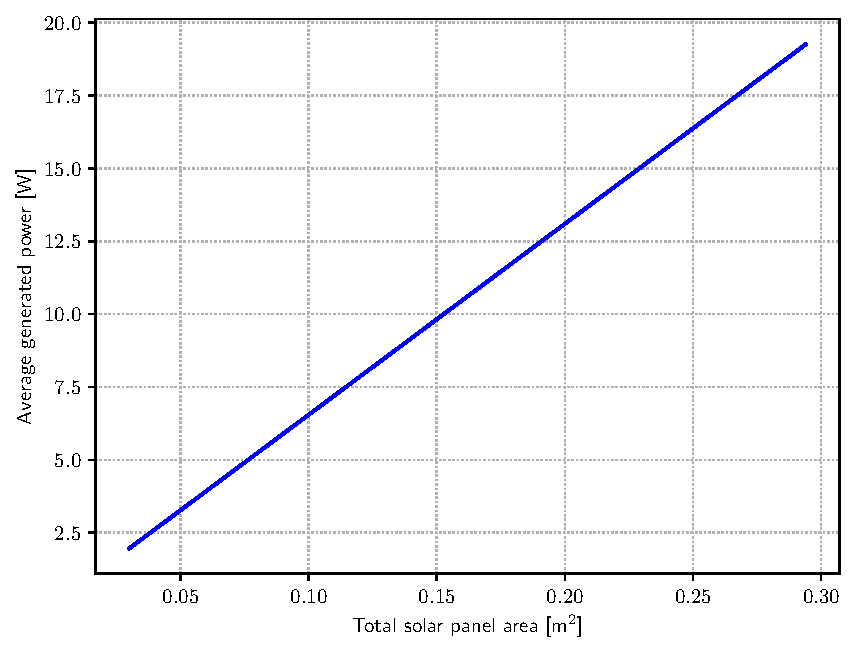
\includegraphics[width=0.8\columnwidth]{curves/sp-area-vs-pwr.pdf}
        \caption{Simulated generated power of the solar panels.}
        \label{fig:sp-area-vs-pwr}
    \end{center}
\end{figure}

Considering the power requirement presented in \autoref{tab:power-duty-cycle}, from the graph of \autoref{fig:sp-area-vs-pwr}, a total solar panel area of approximately 0.1 m$^{2}$ is required for the given system.

%Considerando um satélite sem mecanismos de abertura de painéis solares, ou seja, só com painéis fixos, instalados nas suas faces e cobrindo todas as laterais, a área mínima obtida equivale a um CubeSat entre 3 e 6U. Considerando que o padrão CubeSat não prevê a existência de satélites 4 ou 5U, chega-se ao resultado que é necessário pelo menos um CubeSat de tamanho 6U para esse sistema operando nas condições apresentadas.

%Considerando a possibilidade do uso de mecanismos de abertura de painéis, ou seja, painéis extras que são abertos após o lançamento do satélite, o uso de um CubeSat 3U também seria possível.

Considering a satellite without mechanisms for solar panel deployment, that is, only with fixed panels installed on its faces and covering all sides, the minimum area obtained corresponds to a CubeSat between 3U and 6U. Considering that the CubeSat standard does not provide for the existence of 4U or 5U satellites, the result is that at least a 6U-sized CubeSat is necessary for this system to operate under the presented conditions.

Considering the possibility of using mechanisms for panel deployment, that is, additional panels that are opened after the satellite is launched, the use of a 3U CubeSat would also be possible.

%Desta maneira, para um satélite 6U chega-se aos seguintes resultados da \autoref{tab:sp-power-6u-results} em relação a geração de energia.

In this way, for a 6U satellite, the following results from \autoref{tab:sp-power-6u-results} are obtained regarding power generation.

\begin{table}[!ht]
    \centering
    \begin{tabular}{lc}
        \toprule[1.5pt]
        \textbf{Parameter} & \textbf{Value} \\
        \midrule
        Peak power                  & 15093 mW \\
        Average power (orbit)       & 8688 mW \\
        Average power (sunlight)    & 13770 mW \\
        Orbit period                & 6018 sec \\
        Sun light period            & 3712 sec \\
        Eclipse period              & 2124 sec \\
        \bottomrule[1.5pt]
    \end{tabular}
    \caption{Results of power generation simulation for a 6U CubeSat.}
    \label{tab:sp-power-6u-results}
\end{table}

%O gráfico da \autoref{fig:sp-input-power-6u} ilustra a geração de energia por face e total durante uma órbita completa para o caso considerado.

The curves in \autoref{fig:sp-input-power-6u} illustrates the energy generation per face and total during a complete orbit for the considered case.

\begin{figure}[!ht]
    \begin{center}
        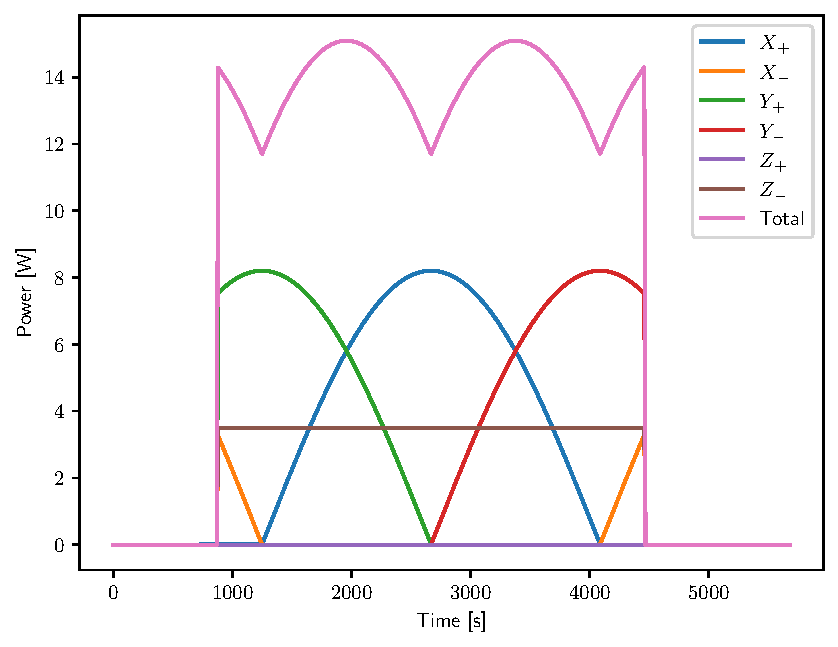
\includegraphics[width=0.8\columnwidth]{curves/sp-input-power-6u}
        \caption{Simulated input power of a 6U CubeSat.}
        \label{fig:sp-input-power-6u}
    \end{center}
\end{figure}

%Por fim, considerando a energia gerada e a consumida, chega-se a uma margem de 2162 mW, ou aproximadamente 25 \%. Esta margem é suficiente considerando-se a degradação dos painéis solares ao longo da missão, e possíveis alteração de projeto, com a remoção de células solares para a instalação de sensores ou antenas. Ou até mesmo a instalação de outros payloads ou subsistemas no mesmo satélite.

Finally, considering the generated and consumed energy, a margin of 2162 mW, or approximately 25 \%, is reached. This margin is sufficient considering the degradation of the solar panels throughout the mission, and possible design changes, such as the removal of solar cells for the installation of sensors or antennas. It also accounts for the installation of other payloads or subsystems on the same satellite.

\section{Possible solutions}

%Nesta seção apresentam-se possíveis soluções para a implementação do trabalho proposto, considerando-se os principais aspectos técnicos necessários para a implementação de um sistema desse tipo conforme as questões apresentadas até então.

In this section, possible solutions are presented for the implementation of the proposed work, considering the main technical aspects necessary for the implementation of such a system, according to the issues presented so far.

\subsection{Clock reference}

As previously mentioned, one of the main sources of error in a GNSS system is the clock reference of the signal transmitter (at the satellite side). In this section, some technologies commonly used in time reference circuits are presented, as well as a discussion of the accuracy of each system and the feasibility of using it in the system discussed here.

%\begin{enumerate}
%    \item Quartz oscilators: $\pm$1 sec a cada 30 dias
%    \item TCXO (Temperature Compensated Crystal Oscillators):
%    \item OCXO (Oven Controlled Crystal Oscillators):
%    \item RbXO (Osciladores de rubídio): $\pm$1 sec a cada 32000 anos.
%    \item Osciladores de césio:
%    \item GPSDO (GPS Disciplined Oscillator):
%\end{enumerate}

\subsubsection{Quartz oscillators (XO)}

%Os osciladores baseados diretamente em cristais como o quartzo, são os tipos de osciladores mais comuns utilizados hoje em die e estão entre os que possuem a menor precisão, perdendo somente para osciladores baseados em circuitos LC. Este tipo pode ser encontrado vastamente no mercado em diversas configurações e tamanho, além de possuir um baixo custo e consumo de energia. Mas em contrapartida é sensível a variações de temperatura, sendo não recomendado para aplicações que requerem alta precisão na frequência de saída. Devido a essas características, este tipo de oscilador não é adequado para ser utilizado como referência para um sistema de GNSS.

Oscillators based directly on crystals such as quartz are the most common types of oscillators used today and are among those with the lowest precision, second only to oscillators based on LC circuits. This type can be widely found in the market in various configurations and sizes, as well as having low cost and energy consumption. However, on the other hand, it is sensitive to temperature variations and is not recommended for applications that require high precision in the output frequency. Due to these characteristics, this type of oscillator is not suitable for use as a reference for a GNSS system.

\subsubsection{Temperature Compensated Crystal Oscillators (TCXO)}

TCXO (Temperature Compensated Crystal Oscillator) is a type of oscillator used in electronic circuits to provide a stable and accurate frequency reference. They work by using a quartz crystal as the resonating element, which vibrates at a specific frequency when electrical voltage is applied to it. This frequency can be used as a reference clock signal for timing and synchronization purposes.

However, the frequency of a quartz crystal is affected by temperature changes, leading to frequency drift and decreased accuracy. To overcome this limitation, TCXOs incorporate a temperature compensation mechanism that adjusts the frequency of the crystal based on the temperature. This can be achieved through various methods, including using a thermistor to measure the temperature and controlling the voltage applied to the crystal, or using a temperature-controlled oven to maintain the crystal at a constant temperature.

The result is a highly stable frequency source that can maintain a high level of accuracy even in harsh operating environments, making TCXOs ideal for use in various applications, such as GPS receivers, cell phones, and other portable devices that require accurate timekeeping.

Despite being significantly more accurate than a common crystal oscillator, this still is not a suitable type to be used as a reference in a GNSS system.

\subsubsection{Oven Controlled Crystall Oscillators (OCXO)}

%OCXOs são osciladores que utilizam uma câmara fechada e com a temperatura controlada para manter a estabilidade em cristais de quartzo. A ideia é manter o cristal em uma temperatura constante para evitar desvios na frequência de oscilação do mesmo por variações de temperatura.

%Devido a característica do controle ativo de temperatura, o consumo energético deste tipo de oscilador é alto em comparação com outros osciladores baseados em cristais. O consumo pode chegar a algumas unidades de watts dependendo da temperatura externa do dispositivo. Normalmente, o cristal é mantido numa temperatura de 75 $^{\circ}$C, por cristais de quartzo apresentarem melhores características de funcionamento nessa faixa. Devido a isso, para aplicações que operam em temperatura ambiente ou baixas temperaturas (como um satélite operando no espaço), o consumo de energia deste tipo de oscilador será elevado.

%Outra característica importante é o seu tamanho, devido ao controle de temperatura, normalmente o volume deste tipo de oscilador é maior dentro da classe dos modelos baseados em cristais, e normalmente não é utilizado em dispositivos portáteis ou baseados em bateria. Apesar destas características, este tipo de oscilador é o que possuí a maior precisão possível dos osciladores baseados em cristais, ficando na faixa entre $2 \times 10^{-8}$ e $5 \times 10^{-7}$ dependendo da faixa de frequência em operação \cite{mancini2004}. Um OCXO instalado em uma placa de circuito impresso pode ser visto na \autoref{fig:ex-ocxo}

OCXOs are oscillators that use a closed chamber with controlled temperature to maintain stability in quartz crystals. The idea is to keep the crystal at a constant temperature to avoid deviations in its oscillation frequency due to temperature variations.

Due to the active temperature control characteristic, the energy consumption of this type of oscillator is high compared to other crystal-based oscillators. Consumption can reach a few watts depending on the external temperature of the device. Normally, the crystal is kept at a temperature of 75 $^{\circ}$C, as quartz crystals exhibit better performance characteristics in this range. Due to this, for applications that operate at ambient or low temperatures (such as a satellite operating in space), the energy consumption of this type of oscillator will be high.

Another important characteristic is its size. Due to the temperature control, the volume of this type of oscillator is usually larger within the class of crystal-based models and is not normally used in portable or battery-based devices. Despite these characteristics, this type of oscillator has the highest possible precision among crystal-based oscillators, ranging between $2 \times 10^{-8}$ and $5 \times 10^{-7}$ depending on the operating frequency range \cite{mancini2004}. An OCXO installed on a printed circuit board can be seen in \autoref{fig:ex-ocxo}.

\begin{figure}[!ht]
    \begin{center}
        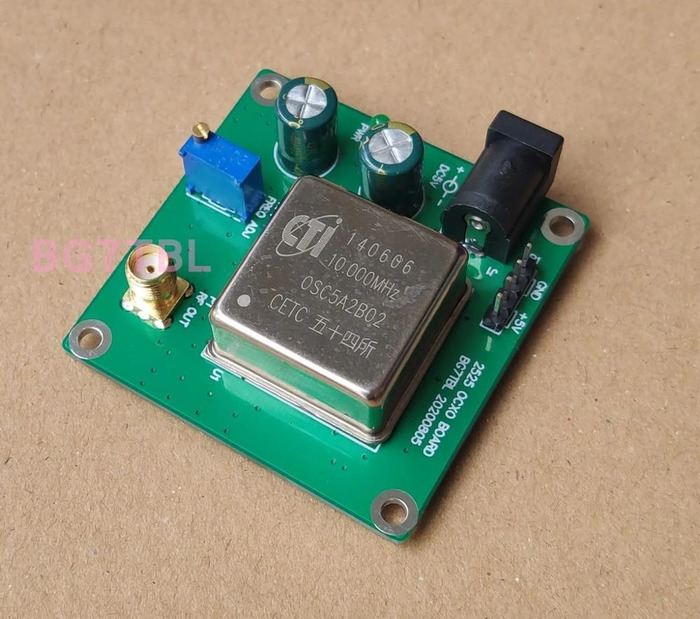
\includegraphics[width=0.5\columnwidth]{figures/ex-ocxo.jpg}
        \caption{OCXO installed on a printed circuit board.}
        \label{fig:ex-ocxo}
    \end{center}
\end{figure}

\subsubsection{Rubidium oscillators (RbXO)}


Rubidium oscillators are a type of frequency reference that use the resonant frequency of rubidium-87 atoms to generate a stable and accurate time signal. They work by confining a cloud of rubidium atoms in a small chamber and applying a magnetic field to the cloud. This magnetic field causes the rubidium atoms to transition between two energy levels, emitting or absorbing light at a very specific frequency, known as the resonant frequency of rubidium-87.

A microwave generator is used to excite the rubidium atoms, and the frequency of the generator is then locked to the resonant frequency of the rubidium atoms. The microwave generator acts as a frequency reference, and the frequency output of the generator can be used as a highly stable and accurate clock signal.

Rubidium oscillators offer a number of advantages over other types of frequency references, including high stability, low aging rate, and low sensitivity to environmental factors such as temperature and pressure changes. They are widely used in a variety of applications, including GPS systems, scientific instrumentation, and telecommunications equipment.

Rubidium oscillators are the cheapest in the class of oscillators used in atomic clocks. They are considered a secondary frequency standard, unlike Cesium oscillators which are more precise and considered primary.

Oscillators of this type are currently readily available on the market, with some examples being the Microchip SA-45S models \cite{sa45s}, which can be seen in \autoref{fig:microchip-csac}.

\begin{figure}[!ht]
    \begin{center}
        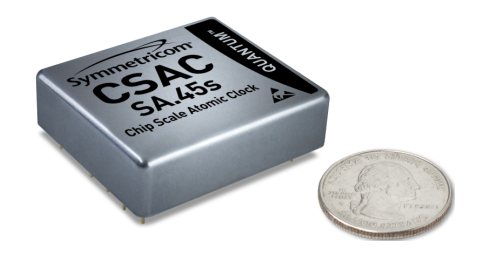
\includegraphics[width=0.7\columnwidth]{figures/microchip-csac}
        \caption{Microchip CSAC SA.45S atomic clock.}
        \label{fig:microchip-csac}
    \end{center}
\end{figure}

Considering factors such as physical size, power consumption, and cost, this type of oscillator is a good option to be considered as a reference for a small satellite-based GNSS system.

\subsubsection{Cesium oscillators}

Cesium atomic clocks are highly precise timekeeping devices that use the vibration frequency of cesium-133 atoms to measure the passage of time. They are considered the standard for time and frequency measurements, as their accuracy is several orders of magnitude better than that of traditional quartz clocks. Cesium atomic clocks are used in a variety of applications, including navigation, telecommunications, and scientific research, and they play a critical role in maintaining Coordinated Universal Time (UTC), the international time standard.

Cesium atomic clocks work by utilizing the vibrational frequency of cesium-133 atoms in a highly controlled environment. The atoms are first excited by a microwave frequency and then allowed to settle into their ground state. As the atoms transition from their excited state to their ground state, they emit electromagnetic radiation at a very specific frequency. This frequency, known as the hyperfine transition frequency of cesium-133, serves as the standard for measuring the passage of time.

In a cesium atomic clock, the atoms are confined in a container called an oven and heated to a high temperature to increase their motion and make the hyperfine transitions easier to detect. The frequency of the microwave radiation that excites the atoms is measured using a sensor called a frequency counter, and this frequency is compared to a reference frequency source to determine the exact time. The whole process is repeated several times per second to maintain a highly accurate and stable measurement of time. The resulting timekeeping system is able to maintain a precision of a few parts in $10^{14}$, making cesium atomic clocks the most accurate timekeepers currently available.



\subsubsection{GPS disciplined oscillators (GPSDO)}

%Um GPSDO, ou GPS disciplined oscillator, é a combinação de um receptor de sinais GPS (ou qualquer outra rede de GNSS) com um oscilador comum, como qualquer um dos tipos citados acima. Normalmente nesse tipo de sistema se utiliza osciladores com maior precisão, como OCXO ou RbXO.

%O funcionamento baseia-se na correção da saída de um oscilador comum utilizando como referência os dados de tempo recebidos de um sistema de GNSS, através do rastreamento do mesmo. Sinais de GPS (ou GNSS) tem uma ótima estabilidade durante longos períodos de tempo, mas devido à limitação dos pulsos a cada segundo presentes no sinal (PPS, Pulse Per Second), o mesmo não possuí um bom desempenho em escalas de tempo curta, como na faixa dos nanosegundos. Dessa forma, utiliza-se um oscilador para obter uma boa resolução em curtos períodos de tempo, e o sinal de GPS para fazer correções em escalas de tempo maiores a medida que o sistema está operando. Combinando as características dois tipos de referência, chega-se a uma precisão final muito próximo osciladores primários como os de Césio.

%A principal desvantagem desse tipo de sistema é a dependência dos sinais de GPS para o seu funcionamento. Para o caso da utilização em uma rede de GNSS, teria-se a limitação de depender do sistema de GPS atual, e teria-se a necessidade dos satélites da rede operarem em órbitas mais baixas que as do satélites de GPS.

%Para sistemas específicos e operando em órbita baixa, esse pode ser uma alternativa viável, desconsiderando questões de dependência em relação a outras redes. Ou ainda, pode se utilizar este tipo de sistema realizar correções em um oscilador já de alta precisão como os osciladores de rubídio.

%Na \autoref{fig:ex-gpsdo} encontra-se um exemplo de modelo comercial de GPSDO baseado em um oscilador OCXO.

A GPSDO, or GPS disciplined oscillator, is the combination of a GPS signal receiver (or any other GNSS network) with a common oscillator, such as any of the types mentioned above. Typically, oscillators with higher precision, such as OCXO or RbXO, are used in this type of system.

The operation is based on correcting the output of a common oscillator using the time data received from a GNSS system, by tracking it. GPS (or GNSS) signals have excellent stability over long periods of time, but due to the limitation of pulses per second (PPS) present in the signal, it does not perform well on short time scales, such as in the nanosecond range. Thus, an oscillator is used to obtain good resolution over short periods of time, and the GPS signal is used to make corrections on larger time scales as the system is operating. By combining the characteristics of both types of references, a final precision is achieved that is very close to primary oscillators such as cesium.

The main disadvantage of this type of system is the dependence on GPS signals for its operation. For the case of use in a GNSS network, there would be a limitation of depending on the current GPS system, and there would be a need for network satellites to operate in lower orbits than GPS satellites.

For specific systems operating in low orbit, this may be a viable alternative, disregarding issues of dependency on other networks. Alternatively, this type of system can be used to make corrections to an already highly precise oscillator, such as rubidium oscillators.

In \autoref{fig:ex-gpsdo} there is an example of a commercial GPSDO model based on an OCXO oscillator.

\begin{figure}[!ht]
    \begin{center}
        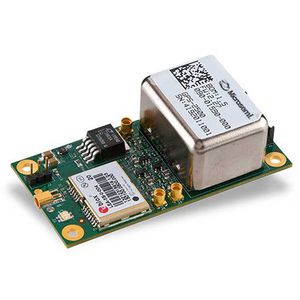
\includegraphics[width=0.5\columnwidth]{figures/gps-2550}
        \caption{Example of a GPSDO based on a OCXO (Microsemi GPS-2550).}
        \label{fig:ex-gpsdo}
    \end{center}
\end{figure}

\subsubsection{Conclusions}

\begin{table}[!ht]
    \centering
    \begin{tabular}{lcccc}
        \toprule[1.5pt]
        \textbf{Oscillator Type} & \textbf{Accuracy} & \textbf{Aging/10 year} & \textbf{Power} & \textbf{Weight} \\
        \midrule
        XO                   & $10^{-5}$ to $10^{-4}$   & 10-20 PPM                                 & 20 $\mu$W  & 20 g \\
        TXCO                 & $10^{-6}$                & 2-5 PPM                                   & 100 $\mu$W & 50 g \\
        MCXO                 & $10^{-8}$ to $10^{-7}$   & 1-3 PPM                                   & 200 $\mu$W & 100 g \\
        OCXO (5 to 10 MHz)   & $10^{-8}$                & $2 \times 10^{-8}$ to $2 \times 10^{-7}$  & \multirow{2}{*}{1-3 W} & \multirow{2}{*}{200-500 g} \\
        OCXO (15 to 100 MHz) & $5 \times 10^{-7}$       & $5 \times 10^{-10}$ to $5 \times 10^{-9}$ &            &  \\
        RbXO                 & $10^{-9}$                & $5 \times 10^{-10}$ to $5 \times 10^{-9}$ & 6-12 W & 1,5-2,5 kg\footnote{\textcolor{red}{Há versões miniaturiazadas.}} \\
        Cs                   & $10^{-12}$ to $10^{-11}$ & $10^{-12}$ to $10^{-11}$                  & 25-40 W & 10-20 kg \\
        GPS                  & $4 \times 10^{-8}$ to $10^{-11}$ & $10^{-13}$ & 4 W & 340 g \\
        \bottomrule[1.5pt]
    \end{tabular}
    \caption{Compasiron between the main types of oscillators \cite{mancini2004}.}
    \label{tab:osc-comp}
\end{table}

\begin{itemize}
    \item Adicionar transmissão de sinais de GNSS às mega-constelações atuais, precisando somente adicionar relógio de alta precisão a cada satélite. Considerando custo e praticidade, essa seria possivelmente a melhor alternativa.
    \item Montar uma rede dedicada, com satélites feitos exclusivamente para emissão de sinais de GNSS. Essa seria solução de maior custo e provavelmente a mais ineficiente em termos de praticidade.
\end{itemize}

\subsection{Radio transmitters}

%Como discutido na \autoref{sec:ionospheric-delay}, uma solução para contornar o problema do atraso ionosférico é a utilização de duas frequências diferentes para a transmissão dos sinais de geolocalização. Com isso, surge a necessidade da utilização de dois transmissores diferentes, ou até mesmo um único transmissor com a capacidade de realizar transmissões em duas frequências distintas.

%Neste caso, não há grandes requisitos técnicos para um transmissor deste tipo. Mas, alguns cuidados devem ser tomados a utilização neste tipo de sistema. Um deles é com o tempo de duração das transmissões, já que em um sistema deste tipo, o rádio deve emitir sinais a todo momento, deste forma o mesmo deve suportar operações ininterruptas. Neste caso, deve-se tomar cuidado com o projeto térmico do mesmo, já em operando desta forma, calor considerável seria gerado o que poderia diminuir a vida útil dos circuitos ou até mesmo danificá-los permanentemente. Ou cuidado a ser tomado, e neste caso especialmente tratando-se da utilização em satélites de pequeno porte, seria em relação ao consumo energético dos transmissores. Considerando transmissões com alta periodicidade ou até mesmo ininterruptas, a eficiência energética do transmissor torna-se extremamente relevante.

%Considerando uma operação nas frequências já utilizadas pelas redes de GNSS atuais, também haveria a necessidade da utilização de transmissores customizados, pois para estas frequências normalmente não se encontra transmissores COTS para satélites no mercado.

%Devido às variações térmicas que um satélite está exposto, também podem ocorrer drifts de frequência no circuito de clock do transmissor, causando variações na frequência dos sinais transmitidos. Desta forma, também deve-se utilizar circuitos com boa precisão. Mas diferentemente dos circuitos de clock da referência de tempo do sistema, altas precisões como a encontrada em relógio de rubídio ou césio, por exemplo, não são necessárias.

%Considerando os aspectos térmicos, energéticos e de operação, uma solução customizada para o rádio transmissor seria a mais indicada. Uma outra possibilidade seria a utilização de um Rádio Definido por Software (SDR), onde neste caso a maior parte das etapas de transmissão poderiam ser implementadas em software.

The solution to overcome the ionospheric delay problem discussed in \autoref{sec:ionospheric-delay} is the use of two different frequencies for geolocation signal transmission. This creates the need for two different transmitters, or even a single transmitter with the ability to transmit on two different frequencies.

There are no major technical requirements for this type of transmitter. However, some precautions must be taken when using it in this type of system. One of them is the duration of transmissions, as the radio must emit signals continuously, so the design must consider the thermal management to avoid reducing the lifespan of the circuits or even damaging them permanently.

Another aspect to consider, especially for use in small satellites, is the energy consumption of the transmitters. Considering transmissions with high periodicity or even continuous, the energy efficiency of the transmitter becomes extremely relevant.

Customized transmitters would be necessary for operation at the frequencies currently used by existing GNSS networks, as COTS transmitters for satellites are not usually available for these frequencies in the market. Due to the thermal variations to which a satellite is exposed, frequency drifts in the transmitter's clock circuit may occur, causing variations in the frequency of the transmitted signals. Therefore, circuits with good precision must be used, but high precision like that found in rubidium or cesium clocks is not necessary.

Considering the thermal, energy, and operational aspects, a custom solution for the transmitter would be the most appropriate. Another possibility would be the use of a Software Defined Radio (SDR), where most of the transmission stages could be implemented in software.

\subsection{Antenna}

%Para as antenas dos transmissores, dependendo da frequência adotada, diferentes geometrias e tipos de antenas podem ser utilizadas. Considerando as frequências utilizadas nos sistemas de GNSS atualmente em funcionamento, antenas do tipo Patch podem ser uma boa opção. Considerando por exemplo satélite seguindo o padrão CubeSat, antenas desse tipo são ideias, pois se adequam ao tamanho físico disponível nesse tipo de satélite, e normalmente não requerem mecânismos de ejeção ou abertuda de componentes, que dificultam o projeto das mesmas e trazem riscos durante a fase de comissionamento do satélite.

%Novamente, considerando o uso das frequências normalmente utilizadas em sistemas de GNSS, há a necessidade do projeto de uma antena customizada, pois normalmente não há disponível no mercado antenas Patch para satélite de pequeno porte e que operem nessa faixa de frequência.

For transmitter antennas, different geometries and types of antennas can be used depending on the adopted frequency. Considering the frequencies used in currently operating GNSS systems, Patch antennas can be a good option. For example, for satellites following the CubeSat standard, these types of antennas are ideal because they fit the physical size available in this type of satellite and usually do not require mechanisms for ejecting or opening components, which can complicate their design and pose risks during the satellite commissioning phase.

Again, considering the use of frequencies typically used in GNSS systems, there is a need for a custom-designed antenna because Patch antennas for small satellites operating in this frequency range are not usually available on the market.

\subsection{Attitude and orbit control}

%Considerando as características já apresentadas, para um sistema como esse, não se tem a necessidade de um sistema de controle de atitude altamente preciso, como por exemplo os tipos empregados em satélites para imageamento. Já que os requisitos de operação em relação a atitude se limitam basicamente a manter as antenas voltadas para o Terra durante toda a órbita, um sistema com baixa precisão já seria suficiente. Possivelmente um sistema de controle ativo com magnetorquers em um satélite pequeno seria suficiente, onde nesse caso pode-se atingir uma precisão de até \textcolor{red}{XX} graus. Para satélites maiores, sistemas com rodas de reação podem ser necessários.

%Já em relação ao controle de órbita, devido a natureza de operação na forma de constelação de sistemas desse tipo, um controle da posição do satélite ao longo da sua órbita é necessário. Manter os satélites da constelação em órbitas específicas e principalmente distantes entre si é um fator importante para o correto funcionamento do sistema, visando principalmente a na ocorrência de zonas mortas, onde não há satélites transmitindo sinais em determinados momentos.

%Para isso, alguns tipos de sistemas podem ser utilizados, como por exemplo propulsores baseados na emissão de íons e/ou propulsores a base de propelentes. Novamente, tratando-se de satélites de pequeno porte, aspectos energéticos e físicos devem ser levados em conta para sistemas desse tipo. Por exemplo, sistemas baseados em propelentes podem ser de difícil utilização, devido ao pouco espaço físico disponível para o armazenamento do material propelente.

Considering the characteristics presented, for a system like this, there is no need for a highly precise attitude control system, such as those used in imaging satellites. Since the attitude operation requirements are limited to keeping the antennas pointing towards Earth throughout the orbit, a low-precision system would be sufficient. An active control system with magnetorquers on a small satellite would possibly be sufficient, where in this case, a precision of up to 20 degrees could be achieved \cite{carrara2017}. For larger satellites, reaction wheel systems may be necessary.

Regarding orbit control, due to the nature of operation in the form of a constellation of systems like this, control of the satellite's position along its orbit is necessary. Maintaining the constellation satellites in specific and mainly distant orbits from each other is an important factor for the correct functioning of the system, mainly aiming to avoid dead zones where no satellites transmit signals at certain times.

For this purpose, some types of systems can be used, such as ion thruster-based and/or propellant-based thrusters. Again, for small satellites, energy and physical aspects must be taken into account for these types of systems. For example, propellant-based systems may be difficult to use due to the limited physical space available for storing the propellant material.

\begin{figure}[!ht]
    \begin{center}
        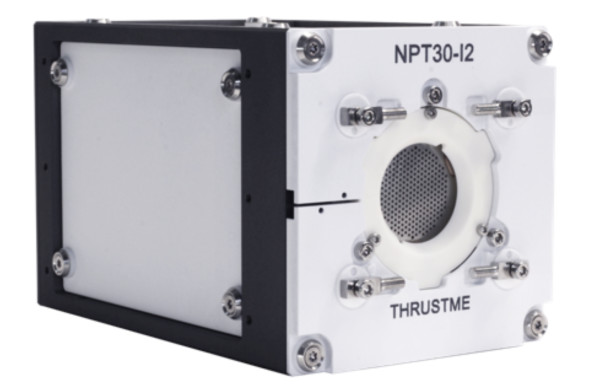
\includegraphics[width=0.5\columnwidth]{figures/npt30-i2}
        \caption{NPT30-I2 ion thruster from ThrustMe.}
        \label{fig:thrustme-npt30-i2}
    \end{center}
\end{figure}

\section{Proposed experiment}

%Como forma de testar o trabalho proposto, propõe-se o desenvolvimento de uma carga útil voltada para pequenos satélites (e neste caso já compatível com o padrão CubeSat). Seguindo o que foi discutido até então, esta carga útil será basicamente um módulo de transmissão de sinais de GNSS, que pode ser integrado a um satélite de pequeno porte. A ideia é que este módulo seja composto por duas placas de circuito impresso que podem ser controlados pelo computador de bordo do satélite, onde o mesmo pode controlar o funcionamento da mesma, e/ou adquirir dados de telemetria a respeito do funcionamento da carga útil.

As a way of testing the proposed work, the development of a payload aimed at small satellites (already compatible with the CubeSat standard in this case) is proposed. Following what has been discussed so far, this payload will basically be a GNSS signal transmission module that can be integrated into a small satellite. The idea is that this module will be composed of two printed circuit boards that can be controlled by the satellite's onboard computer, where it can control its operation and/or acquire telemetry data about the payload's operation.

%Um diagrama de blocos preliminar do módulo proposto pode ser visto na \autoref{fig:payload-block-diagram}. Na \autoref{fig:payload-block-diagram-radios}, há um detalhamento da segunda placa da carga útil, que é composta pelos elementos de radio frequência.

A preliminary block diagram of the proposed module can be seen in \autoref{fig:payload-block-diagram}. In \autoref{fig:payload-block-diagram-radios}, there is a breakdown of the second board of the payload, which is composed of radio frequency elements.

\begin{figure}[!ht]
    \begin{center}
        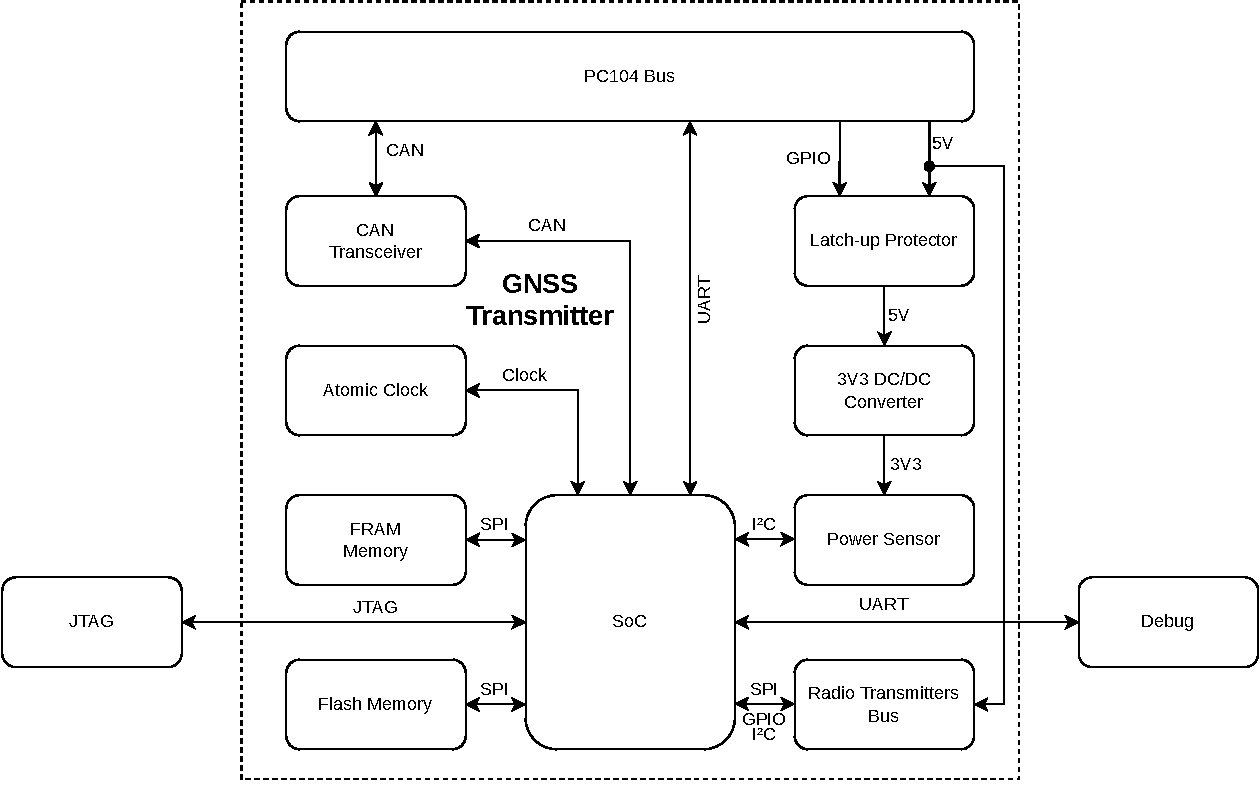
\includegraphics[width=\columnwidth]{figures/block-diagram}
        \caption{Preliminary block diagram of the proposed payload.}
        \label{fig:payload-block-diagram}
    \end{center}
\end{figure}

\begin{figure}[!ht]
    \begin{center}
        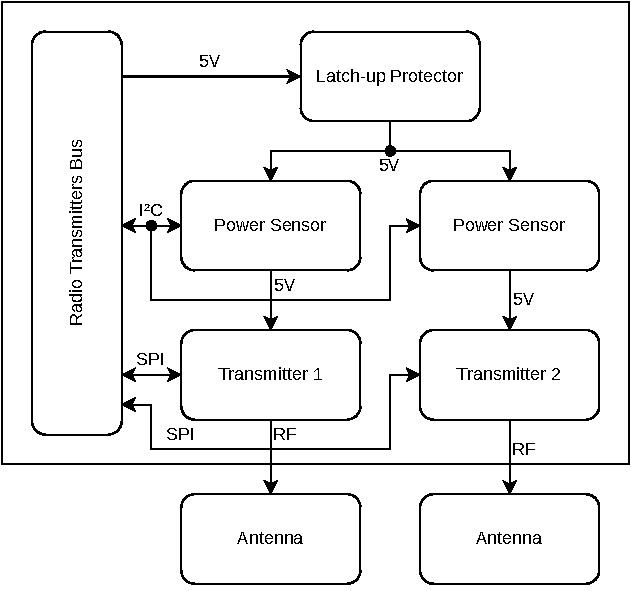
\includegraphics[width=0.6\columnwidth]{figures/radios-block-diagram}
        \caption{Preliminary block diagram of the radio transmitters module.}
        \label{fig:payload-block-diagram-radios}
    \end{center}
\end{figure}

%Como pode ser visto nos diagrama, seguindo algumas características comuns em cargas úteis voltadas para CubeSats, pretende-se utilizar um ou mais barramentos de 5 V para a alimentar todo o conjunto. A comunicação de dados com o restante do satélite (computador de bordo neste caso) poderá ser feita tanto através de um barramento CAN, quanto através de um barramento RS-485. Todas essas entradas e saídas através de um barramento do tipo PC104.

As can be seen in the diagram, following some common characteristics in payloads aimed at CubeSats, one or more 5V buses will be used to power the entire assembly. Data communication with the rest of the satellite (onboard computer in this case) can be done through either a CAN bus or an RS-485 bus. All of these inputs and outputs through a PC104 bus.

%Internamente, a linha de alimentação será composta num primeiro estágio por um proteto contra latch-up, que limitam a corrente de entrada do circuito e protegem contra possíveis surtos de corrente causados por radiação solar e que podem danificar permanentemente o módulo. Desta forma, a adição de uma proteção contra latch-ups pode aumentar o tempo de funcionamento dos elementos do circuito \cite{botma2013}. Após esta etapa, encontra-se um conversor DC/DC que abaixa os 5 V de entrada para 3.3 V, que é a tensão de alimentação principal da maior parte dos elementos da placa. Após a etapa de conversão de tensão, encontra-se um sensor de tensão e corrente, que permite acompanhar o consumo de energia da parte de processamento e controle do módulo. Este sensor é controlado e acessado pelo processador principal do módulo.

Internally, the power line will be composed in a first stage by a latch-up protection, which limits the input current of the circuit and protects against possible current surges caused by solar radiation that can permanently damage the module. Thus, adding latch-up protection can increase the operating time of the circuit elements. After this stage, there is a DC/DC converter that lowers the 5V input to 3.3V, which is the main supply voltage for most of the board's components. After the voltage conversion stage, there is a voltage and current sensor that allows monitoring of the processing and control part's energy consumption. This sensor is controlled and accessed by the module's main processor.

%Para a parte de controle, será utilizado um SoC (System-on-a-chip) composto por um microcontolador e um FPGA. O modelo exato do mesmo ainda está sob análise. Este elemento será responsável por coordenar todo o funcionamento da carga útil, e por realizar a comunicação com o computador de bordo do satélite.

For the control part, a SoC (System-on-a-chip) composed of a microcontroller and an FPGA will be used. The exact model is still under analysis. This element will be responsible for coordinating the entire payload's operation and for communicating with the satellite's onboard computer.

%Na parte de memórias externas, será utilizado prelinimarmente um memória RAM do tipo FRAM, para armazenamento de dados críticos da carga útil (como por exemplo parâmetros de configuração). Também pretende-se utilizar uma memória flash do tipo NAND para armazenamento de dados em massa (neste caso, dados de telemetria).

For external memory, an FRAM type RAM will be preliminarily used to store critical payload data (such as configuration parameters). It is also intended to use a NAND flash memory for mass data storage (in this case, telemetry data).

%Na parte de sensoriamento, como já citado anteriormente, pretende-se utilizar um sensor de tensão e corrente, além de um sensor de temperatura instalado próximo ao circuito de referência de clock.

For sensing, as mentioned earlier, a voltage and current sensor will be used, as well as a temperature sensor installed near the clock reference circuit.

%Já na parte do circuito de referência de clock, será utilizar um relógio atômico de rubídio, como já discutido anteriormente neste capítulo. O sinal de referência gerado alimentará um circuito digital implementado no FPGA do SoC utilizado, e servirá como referência para o relógio interno do sistema.

In the clock reference circuit part, a rubidium atomic clock will be used, as discussed earlier in this chapter. The reference signal generated will feed a digital circuit implemented in the SoC's FPGA used and serve as a reference for the system's internal clock.

%Além disso, a placa também terá transceptores para os barramentos de comunicação: CAN e RS-485.

In addition, the board will also have transceivers for communication buses: CAN and RS-485.

%Já na parte de transmissão dos sinais de rádio frequência, devido a limitações de espaço físico, pretende-se utilizar uma segundo placa acoplada a principal através de um barramento. Esta placa conterá os dois transmissores de rádio do sistema, juntamente com um protetor de latch-up exclusivo para o conjunto, e um sensor de corrente e tensão para cada transmissor, que servirá para acompanhar o funcionamento dos mesmos. Na saída dos transmissores, haverá conectores coaxiais que serviram para conector uma antena ao conjunto. Como estes transmissores irão irradiar sinais com uma potência relativamente elevada, um cuidado especial com a dissipação térmica do mesmo deverá ser levado em conta. Dissipadores de metal deverão ser instalados ao conjunto para dissipar o calor gerado por condução términa. Um sensor de temperatura instalado nesse dissipador poderá auxiliar no monitoramento da temperatura, podendo até servir como alarme e um possível desligamento em caso de superaquecimento do sistema. Problemas de temperatura serão críticos nesse módulo devido principalmente a natureza de um sistema de GNSS: os sinais são transmitidos o tempo todo.

For radio frequency signal transmission, due to physical space limitations, a second board attached to the main one via a bus will be used. This board will contain the system's two radio transmitters, along with an exclusive latch-up protector for the assembly and a voltage and current sensor for each transmitter, which will serve to monitor their operation. At the transmitter's output, there will be coaxial connectors that will connect an antenna to the assembly. As these transmitters will radiate signals with a relatively high power, special care must be taken with their thermal dissipation. Metal heat sinks should be installed on the assembly to dissipate the heat generated by thermal conduction. A temperature sensor installed in this heat sink will allow monitoring the temperature of the system.

%Para auxiliar na proteção contra radiação espacial e na dissipação térmica de todo o módulo, todas as placas serão instaladas dentro de um case de metal (preliminarmente alumínio).

To assist in protection against space radiation and thermal dissipation of the entire module, all boards will be installed within a metal case (preliminarily aluminum).

%Por fim, como já citado, o módulo proposto e descrito ainda encontra-se em fase preliminar de definição, e pode sofrer alterações de acordo com o andamento do trabalho e com resultados preliminares obtidos.

Finally, as already mentioned, the proposed and described module is still in a preliminary stage of definition, and may undergo changes according to the progress of the work and preliminary results obtained.
    %
% conclusion.tex
%
% Copyright (C) 2023 by Universidade Federal de Santa Catarina.
%
% Towards the Conception of GNSS Networks Based on Small Satellites
%
% This work is licensed under the Creative Commons Attribution-ShareAlike 4.0
% International License. To view a copy of this license,
% visit http://creativecommons.org/licenses/by-sa/4.0/.
%

%
% \brief Conclusion chapter.
%
% \author Gabriel Mariano Marcelino <gabriel.mm8@gmail.com>
%
% \version 1.1.0
%
% \date 2019/11/30
%

\chapter{Next steps} \label{ch:conclusion}

As a conclusion of this preliminary stage, based on the analysis carried out so far, the implementation of the proposed system appears to be feasible.

As next steps, we intend to refine the analyses conducted so far. In addition, an orbit analysis will be added to determine the number of objects required for different types of orbits. As well as the minimum number of satellites required to achieve a certain accuracy considering a receiver being operated by a user of the system.

We also plan to develop the design of the proposed payload for a possible future implementation and deployment in one of the research group's future missions. To effectively test the proposed system and developed payload, a mission composed of multiple satellites will also be presented and proposed.

% #############################################################################
% #############################################################################
% #############################################################################
% #############################################################################

\section{Schedule}

\textcolor{red}{TODO}

The activities scheduled for the completion of the work can be seen in \autoref{tab:schedule}, where the detailed description of each activity is found just below.

\begin{table}[!ht]
    \centering
    \begin{tabular}{lc}
        \toprule[1.5pt]
        \textbf{Activity} & \textbf{Month} \\
        \midrule
        & \\
        \bottomrule[1.5pt]
    \end{tabular}
    \caption{Scheduled activities for the completion of the work.}
    \label{tab:schedule}
\end{table}

\begin{itemize}
    \item .
\end{itemize}
    %
% references.tex
%
% Copyright (C) 2022 by Universidade Federal de Santa Catarina.
%
% GNSS Networks Based on Small Satellites
%
% This work is licensed under the Creative Commons Attribution-ShareAlike 4.0
% International License. To view a copy of this license,
% visit http://creativecommons.org/licenses/by-sa/4.0/.
%

%
% \brief References section.
%
% \author Gabriel Mariano Marcelino <gabriel.mm8@gmail.com>
%
% \version 0.1.0
%
% \date 2019/11/30
%

\bibliographystyle{unsrt}

\bibliography{references/floripasat2,%
              references/nanosatseu,%
              references/aarestad2020,%
              references/xona-space,%
              references/sa45s,%
              references/beidou,%
              references/glonass,%
              references/gps,%
              references/qzss,%
              references/irnss,%
              references/larson2005,%
              references/marino2016,%
              references/cds,%
              references/thombre2015,
              references/gps-standard}


\end{document}
